\documentclass{article}
\usepackage{graphicx}
\graphicspath{ {./img/} }
\usepackage{setspace}
\usepackage{amssymb}
\usepackage{amsmath}
\usepackage{chngcntr}
\usepackage{float}
\usepackage{tabu}
\usepackage{bm}
\usepackage[lite]{amsrefs}

\counterwithin*{equation}{section}

\newcommand{\R}{\mathbb{R}}

\makeatletter
\newcommand*\bigcdot{\mathpalette\bigcdot@{1}}
\newcommand*\bigcdot@[2]{\mathbin{\vcenter{\hbox{\scalebox{#2}{$\m@th#1\bullet$}}}}}
\makeatother

\newcommand{\qed}{\hfill$\square$}

\usepackage{afterpage}

\newcommand\blankpage{%
    \null
    \thispagestyle{empty}%
    \addtocounter{page}{-1}%
    \newpage}


\begin{document}


\title{Introduction to Probability (notes)}
\author{Blitzstein, Hwang}
\date{}

\maketitle

\section{Probability and Counting}

	\subsection{Sample Space and Pebble World}
	
		Pretty simple stuff - sample space of all outcomes. Events are subsets of the sample space. Use set notation for the whole jazz, with some booleans thrown in if the outcomes are binary. Leads to naive definition of probability.
		
	\subsection{Naive definition of probability}
	
		$$P_{naive}(A) = \frac{|A|}{\vert S\vert}$$
		
		
	\subsection{How to Count}
	
		\subsubsection{Multiplcation rule}
	
			Multiplication rule: if an experiment is made up of two sub-experiments $A, B$, then the number of outcomes in the whole thing is $\vert A\vert \cdot \vert B\vert$. 
		
			The visualization tool for this is imagine building a tree, and that the branching factor of each new layer is equal to the corresponding experiment being carried out. For instance, if $\vert A\vert = 3$, $\vert B\vert = 4$, then the branching factor of the first layer may be 3 and the branching factor of the second layer may be 4 (or vice versa, it would yield an identical result).
		
		\subsection{Adjustment for overcounting}
		
			So the multiplication rule gives us a way of counting in cases where We sample \textbf{with replacement and care about order} ($n^k$ where $n$ is the number of choices and $k$ is the number of samples taken).
			
			Now say We sample \textbf{without replacement and care about order}, the multiplication rule still has us covered: $\prod_{i=0}^k n - i$. That can also be thought of as adjustment for overcounting: $\frac{n!}{(n-k)!}$.
			
			Now, say, We sample \textbf{without replacement and do not care about order}. How would one go about it? Well, We can already sample without replacement while caring about order, so We just adjust for the overcounting due to caring bout order: each sample has $k$ elements in it, and so We are overcounting each sample $k!$ number of times, yielding $\frac{n!}{(n-k)!k!}$. This is known as the \textbf{binomial coefficient}, or \textbf{n choose k}, which can be written as $\binom{n}{k}$.
		
			To visualize this w.r.t. the product-rule tree, note that You may have a \textit{reduction} in the number of branches in a layer, namely if You've overcounted, the layer adjusting for overcounting of the "tree"\footnote{No longer really a tree since it's not acyclic anymore} would join multiple leaves into one. For instance, if You count the number of ways the letters "AAS" may be arranged, You simply pick where the S is (and the answer is therefore 3 ways), or You can count all samples without replacement $3!$, and then divide by the fact that the two A's are interchangeable: $\frac{3\cdot 2 \cdot 1}{2 \cdot 1} = 3$. Visually:
		
			\begin{figure}[H]
				\caption{Beautiful rendition of adjustment for overcounting}
				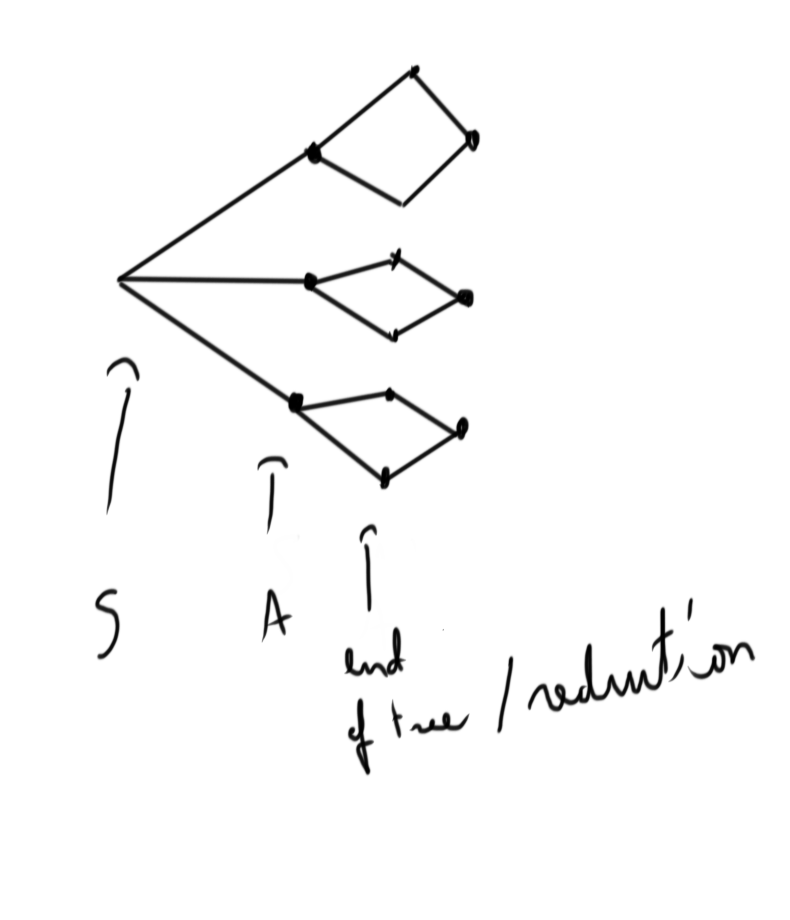
\includegraphics[scale=0.25]{visual_adjustment_for_overcounting}
			\end{figure}
		
		\textbf{Binomial theorem} by the way, goes like this:
		
		$$ (x+y)^n = \sum^n_{k=0} \binom{n}{k} x^ky^{n-k} $$
		
		The story proof/intuition for this isn't so bad. Imagine expanding the $(x+n)^n$ term into $(x+y)(x+y)(x+y)...$. Now, when doing the multiplication, You'll expand one bracket at a time - each time You'll choose either the x or the y to multiply out (i.e. $(x+y)(x+y)(x+y) \implies x(x+y)(x+y) + y(x+y)(x+y)$ etc.). Then, in the end, You'll add all the terms with similar powers of x and y to get the coefficient. But, of course, the coefficient for $x^ky^{n-k}$ is just the number of ways to do the expansion while choose $x$ k times (the expansion, in one instance then becomes $xxxyxxyxyxyxx....$ until $k$ $x$'s are obtained).
		
		\textbf{Sampling with replacement and without order} is pretty simple if You, well, have the answer and the correct way of looking at it:
		
		Goes like this: to model replacement, imagine $n$ distinct boxes. To imagine sampling without order, imagine that You're putting $k$ \textit{indistinguishable} balls into the $n$ boxes. Since the balls are indistinguishable, putting them in any order counts as the same sample, so long as the number of balls in each corresponding box is identical as it was before (balls can be swapped out without effect).
		
		Cool, now, We think about an \textit{encoding} for this problem: We can encode this thing with the symbols $\vert$ and \textbf{$\bigcdot$}. First, observe  that any valid encoding will have to begin and end with $\vert$. Then, observe that for n boxes, the number of $\vert$ in between will be $n-1$ (for instance, two boxes are $\vert \cdot \vert \cdot \vert$, yielding one $\vert$ in between). Finally, We will have $k$ balls to put into the boxes, which means that the total number of symbols in between the ending and beginning $\|$'s will be $k + n - 1$. All that remains to do is to count the number of ways to choose the positions for the $\bigcdot$ symbols, without order. This then of course just leads $\binom{n+k-1}{k}$.
		
		In summary then:
		
		\begin{center}
			\begin{tabu}{|c | c | c |}
				\hline 
				$\frac{Replacement}{order}$ & With & Without \\
				\hline
				With & $n^k$ & $\frac{n!}{(n-k)!}$ \\
				\hline
				Without & ${ n+k-1 \choose k}$ & $\frac{n!}{(n-k)!k!}$ \\
				\hline	
			\end{tabu}
		\end{center}
		
	\subsection{Story Proofs}
	
		Story proofs just refer to a more "colloquial" style of proofs. They prove stuff by showing that two different ways of counting stuff is actually just counting the same stuff. For example:
		
		The claim is that $${n \choose k} = {n \choose n-k}$$ 
		
		The story proof is as follows: imagine You are picking a team of size $k$ out of $n$ players. But, instead of choosing the $k$ players that make the team, You could instead choose the $n-k$ players that don't make the team! And so ${n \choose k} = {n \choose n-k}$. \hfill $\square$
		
		Another example:
		
		 $$n {n-1 \choose k-1} = {n \choose k} k$$
		 
		 For which a good story is the following: imagine picking a team of size $k$ out of $n$ players, and then choosing one of those $k$ players to be the captain. One way to do this is to choose the captain (n choices), and then choose the rest of the team ${ n-1 \choose k-1}$. Another way of doing the same thing is to first choose the team ${ n \choose k}$ and then choose the captain among them, and the captain can be any one of the $k$ players yielding ${ n-1 \choose k-1}k$. \hfill $\square$
		 
		 Another example (Vandermonde's identity):
		 
		 $${m + w \choose k} = \sum_{j=0}^k {m \choose j}{ w \choose k-j}$$
		
		The story is as follows: say You are picking a committee of size $k$ out of a group of $m$ men and $w$ women. The number of ways to do this then is of course ${m + w \choose k}$. Another way of counting the same thing is to think that if there are $j$ men in the committee, there must be $k-j$ women! So You count the number of ways there are to have no men, one man... k men in the committee, and some all of those ways up\footnote{You may say "but what if k, the number of committee members, is larger than m, the number of men? Turns out ${m \choose k}$ where $m < k$ is defined as 0. So when $j=0$, We will account for all possible all-women committees, and then iterate through the ones with men in them, until the number of men becomes impossible, and multiplying by 0 resulting from ${m \choose j}$ and $j > m$ will cancel those terms out.}. This of course also means that $${m + w \choose k} = \sum_{j=0}^k {w \choose j}{ m \choose k-j}$$
		\hfill $\square$
		
		Another example: 
		
		$$\frac{(2n)!}{2^n\cdot n!} = (2n-1)(2n-3)(2n-5)\cdots(3)(1) = \prod^n_{j=1} (2n -2j + 1)$$
		
		And now for the story: imagine You've got $2n$ people, and You're wondering how many two-person partnerships can be made out of this group of people. One way to do this would be to start counting would be to count all possible permutations (without replacement, with order) yielding $(2n)!$ permutations, and then counting each adjacent couple (person 1 and 2 are together, 3 and 4 etc.). Then You can adjust for overcounting by noting that the order of the people \textit{in} in the couple doesn't matter ($AB = BA$), and there are $n$ couples yielding and overcounting factor of $2^n$, and that the ordering of the couples themselves does not matter ($AB\vert CD = CD\vert AB$), and since there are $n$ couples this yields an overcounting factor of $n!$, which all together yields $\frac{(2n)!}{2^n\cdot n!}$ . 
		
		An alternative approach is to observe that the first person has $2n-1$ options for a partner, the second person has $(2n-3$ options for a partner and so on, yielding the right hand side. \hfill $\square$
		
	\subsection{Non-naive definition of probability}
	
		So We define some function that takes events to probabilities $P$. Under the hood this is measure theory stuff, but I guess We'll just come back for that at some point.
		
		Anyway, the function has to satisfy some basic axioms:
		
		$$P(\emptyset) = 0, P(S) = 1$$
		
		where $S$ is the sample space. The other import axiom is:
		
		For $A_1, A_2\cdots$ disjoint events $P(A_i) \cap P(A_j) = 0, i \neq j$:
		
		$$P\left(\bigcup^\infty_{i=1} A_i \right) = \sum^\infty_{i=1} P\left( A_i \right)$$
		
		And everything else can be derived from those two, apparently.
		
		\textbf{Frequentist} perspective on $P(A)$ is that $P(A)$ is the fraction of times A would occur if We were able to repeat experiments an infinite number of times. \textbf{Bayesian} perspective is that $P(A)$ reflects our \textit{prior belief} that $A$ will occur - how likely We think $A$ is. They're kind of similar, in a way.
		
	\subsection{Worked story proofs}
	
		\textbf{Q15}
			$$\sum^n_{k=0} {n \choose k} = 2^n$$
			
			Alright. So, on the left, You're counting the number of ways to pick a team of size k out of n people. Equivalently, each person is either in or out, giving $2^n$ \hfill$\square$
			
		\textbf{Q16}
		
			For all positive integers $n$ and $k$ with $n \ge k$,
			
			$${n \choose k} + {n \choose k-1} = {n + 1 \choose k} $$
			
			Algebraic proof: 
			
			$$\frac{n!}{(n-k)!k!} + \frac{n!}{(n+1-k)!(k-1)!} = \frac{(n+1)!}{(n+1-k)!k!}$$
			
			$$\frac{n!(n+1-k)!(k-1)!}{(n-k)!k!(n+1-k)!(k-1)!} + \frac{n!(n-k)!k!}{(n+1-k)!(k-1)!(n-k)!k!} = \frac{(n+1)!}{(n+1-k)!k!}$$
			
			$$\frac{n!(n+1-k)!(k-1)! - n!(n-k)!k!}{(n-k)!k!(n+1-k)!(k-1)!} = \frac{(n+1)!}{(n+1-k)!k!}$$
			
			$$\frac{(n+1-k)!(k-1)! - (n-k)!k!}{(n-k)!k!(n+1-k)!(k-1)!} = \frac{n+1}{(n+1-k)!k!}$$
			
			$$\frac{(k-1)!((n+1-k)! - (n-k)!k)}{(n-k)!k!(n+1-k)!(k-1)!} = \frac{n+1}{(n+1-k)!k!}$$
			
			$$\frac{(n+1-k)! - (n-k)!k}{(n-k)!k!(n+1-k)!} = \frac{n+1}{(n+1-k)!k!}$$
			
			$$\frac{(n-k)!((n+1-k) - k)}{(n-k)!k!(n+1-k)!} = \frac{n+1}{(n+1-k)!k!}$$
			
			$$\frac{(n+1-k) - k}{k!(n+1-k)!} = \frac{n+1}{(n+1-k)!k!}$$
			
			$$\frac{n+1}{k!(n+1-k)!} = \frac{n+1}{(n+1-k)!k!}$$
			
			\hfill$\square$
			
			Story-proof: Out of $n+1$ people, You're choosing one group of size $k$. Equivalently, You could have counted the number of ways to choose $n$ out of $k$ people which strictly excludes one dude from the pool, and add the number of ways to choose a team of size $k-1$ out of the $n$, where the final $k$'th dude is the removed one.
			
			Or, maybe, more clearly, on the right, You're choosing a team such that the excluded guy doesn't appear ${n \choose k}$ and a team that strictly includes the previously excluded guy ${n \choose k-1}$. \hfill$\square$ 
			
			\hfill
			
		\textbf{Q18}
		
			$${k \choose k} + {k + 1 \choose k} + {k + 2 \choose k} + \cdots + {n \choose k} = {n+1 \choose k+1} $$
			
			Well, on the right, We are choosing a group of $k+1$ people out of $n+1$ people, cool. 
			
			On the left, then, ${n \choose k}$ is selecting $k$ people out of $n$ options. 
			
	\subsection{Naive definition of probability exercises}
	
		\textbf{Q22}
		
			6 kids, 3 girls, 3 boys, what's the likelihood that the 3 eldest are girls?
			
			All birth orders are equally likely, so total number of birth orders $6!$. We are interested in the first 3 being girls, which has $3!$ ways of happening, and the rest can be whatever way, so another $31$, giving a total of $3! \cdot 3!$. So then the probability is $\frac{3!\cdot 3!}{6!} = 0.05$.
			
			Now, how to do it with choices? There are ${6 \choose 3}$ arrangements of the births. Only one of those is the interesting one, so, the answer then is ${6 \choose 3}^{-1} = 0.05$ \qed
			
			\hfill
			
		\textbf{Q23}
		
			6 districts, 6 robberies, what are the chances of one district having more than one? Better question to ask, what is the probability of having zero or one robberies.
			
			$$1 - \frac{6!}{6^6}$$
			
			\hfill
			
		\textbf{Q26}
		
			Student chooses 3 courses, each of which had some random time slot out of 10 timeslots. The probability of there not being a conflict is $\frac{9}{10} \cdot \frac{8}{10} = \frac{72}{100}$. So the compliment is $\frac{28}{100}$.
			
			Total number of possibilities that fit the event: $10 \cdot 9 \cdot 8$. Total sample space is $10 \cdot 10 \cdot 10$. The probability then is $1 - \frac{10 \cdot 9 \cdot 8}{1000} = 0.28$.
			
			\hfill
			
		\textbf{Q27}
		
		(a) 21 is more likely than 22.
		
		(b) equal due to symmetry.
		
		\hfill
		
		\textbf{Q28}
		
			r red balls, g green balls.
			
			(a) A priori, all balls are equally likely to be chosen at any point. 
			
			(b) Aight, so probability of the first one happening is $\frac{g}{r+g}$.
			
			Probability of the second one happening is gg + rg: $\frac{g}{r+g} \cdot \frac{g-1}{r+g-1} + \frac{r}{r+g} \cdot \frac{g}{r+g-1} $
			
			$$\frac{g}{r+g} \cdot \frac{g-1}{r+g-1} + \frac{r}{r+g} \cdot \frac{g}{r+g-1} $$
			
			$$\frac{g(g-1) + rg}{(r+g)(r+g-1)} $$
			
			$$\frac{g^2 - g + rg}{(r+g)(r+g-1)} $$
			
			$$\frac{g(g - 1 + r)}{(r+g)(r+g-1)} $$
			
			$$\frac{g}{(r+g)} $$
			
			And as a final note, P(rg) = P(gr). Ultimately, any permutation is equally likely here, since the order of events doesn't really matter because of the aforementioned symmetry. 
			
			(c) Probability that the balls are the same is the same as the probability that the balls are different. So P(gg) = P(rg) = P(gr) = P(gg). 
			
			Well, algebraically, this is
			
			$$\frac{g}{r+g} \cdot \frac{g-1}{r+g-1} + \frac{r}{r+g} \cdot \frac{r-1}{r+g-1} = 2 \cdot \frac{r}{r+g} \cdot \frac{g}{r+g-1}$$
			
			$$g(g-1) + r(r-1) = 2rg$$
			
			$$g(g-1) + r(r-1) - 2rg = 0$$
			
			$$g^2 - g + r^2 -r - 2rg = 0$$
			
			$$(g-r)^2  -g -r = 0$$
			
			$$(g-r)^2 = r + g$$
			
			$$(g-r)^2 = 16$$
			
			So $r = 10, g = 6$ or vice versa.\qed
			
			\hfill
			
			\textbf{32}
			
			(a) Draw 5 cards, out of 52, 13 of each suit. Probability that they are all the same. Well, overall combos are just $\binom{52}{5}$. Then choose one suit, and 5 cards out of it, dismiss the royal flush and You get:
			
			$$\frac{4\cdot\left(\binom{13}{5} - 1\right)}{\binom{52}{5}}$$
			
			(b) Two of card a, two of card b and a c. There are 13 cards in each suit, and 4 suits, so We have $13\cdot\binom{4}{2}$ ways of getting the first two, and $12\cdot\binom{4}{2}$ and the kicker is any of the other ranks so $52-4-4 = 44$. We overcount here by 2 since the order of the choice of suits does not matter. In total then I wanna say We get
			
			$$\frac{13\cdot\binom{4}{2}\cdot 12\cdot\binom{4}{2} \cdot 44}{2\cdot\binom{52}{5}}$$
			
			Alternatively, You can do this cleaner by choosing two suits, then choosing the cards for each suit:
			
			$$\frac{\binom{13}{2}\cdot\binom{4}{2}^2\cdot 44}{\binom{52}{5}}$$
			
			The two are equal. \qed
			
			\hfill
			
	\subsection{Axioms of probability}
		
		\textbf{46}
			
			Aight, so, ya boy Arby thinks $P(A \cup B) \neq P(A) + P(B)$, where A and B are disjoint.
			
			Alright, well, let's assume one direction of the inequality: $P(A \cup B) < P(A) + P(B)$, since the other way is impossible lol.
			
			We can just buy these kinds of things up from ya boy Arby.  This is actually an equality, but Arby fucked up. Therefore, Arby should be undervaluing the left hand side, so We should buy intersection events and fleece the guy or whatever. 
			
	\newpage
\section{Conditional Probability}
			
	\subsection{Definition and intuition}
		
		Without further ado, for some events A and B where $P(B) > 0$:
			
		$$ P(A\vert B) = \frac{P(A\cap B)}{P(B)}$$
			
		So what is going on in that equation. The left side is saying "this is the probability of A assuming B is true/has happened/will happen/etc. The right side is a fraction whose denominator is $P(B)$, and that is there because We are now changing out sample space S. Think about it - We know that $B$ has happened \textit{for sure}, so now that We know that, out sample space has changed to exclude anything that doesn't include $B$ having happened. Now that We've adjusted the sample space, it still might be the case that $A$ \textit{can} happen, it's just that $B$ had to have happened too. The probability of that event is just $P(A\cap B)$.
			So, in short, probability of A given B is just the probability of both $A$ and $B$ happening, given that $B$ \textit{has} happened. If You're looking for more intuition, draw out a few venn diagrams, or read this\footnote{https://www.countbayesie.com/blog/2015/2/18/bayes-theorem-with-lego} blog entry.
			
	\subsection{Bayes' Rule and the law of total probability}
		
		\textbf{Generalized intersection probabilities}
			
			So, We take the fact that 
				
			$$P(A\cap B) = P(B)P(A\vert B) = P(A)P(B\vert A)$$
				
			Which works since $P(B)$ is in the "original" sample space, and then We  take a fraction of it to get $P(A\cap B)$ which is still in the "original"/unconditioned sample space. Same thought process for $P(A)P(B\vert A)$.
				
			The generalized version is that You can just keep doing that:
				
			$$P(A_1\cap A_2\cap\cdots\cap A_n) = P(A_1)\cdot P(A_2\vert A_1) \cdot P(A_3\vert A_2\cap A_1)\cdots P(A_n\vert A_{n-1}\cap\cdots A_1)$$
				
			And You can rearrange the left hand side events whatever way You like e.g. $P(A_n)\cdot P(A_3 \vert A_n)\cdots$ etc.
				
		\newpage
				
		\textbf{Bayes' Rule}
			
			$$P(A\vert B) = \frac{P(B\vert A)P(A)}{P(B)} = \frac{P(B\cap A)}{P(B)}$$
				
			Nothing too incredible here, just another way of writing the intersection.
				
		\hfill
			
		\textbf{Odds}
			
			$$odds(A) = \frac{P(A)}{P(A^c)}$$
				
			So what the hell \textit{are} odds anyway. They are the ratio of the probability of A happening to the probability of A \textit{not} happening. For instance, if $P(A) =  \frac{2}{3}$, then the odds of A happening are 2:1: A is twice as likely to happen than it is to not happen. Great.
				
			Now, say We have the odds and want to get back to just a straight forward $P(A)$. That is just:
				
			$$P(A) = \frac{odds(A)}{odds(A) + 1}$$
				
			Why is that You may say. It's because $odds(A)+1$ is the sample space since the odds are always "x to one". So all $odds(A)$ gives us is the fraction of the sample space favourable to $A$ normalize by $P(A^c)$.
				
		\hfill
				
		\textbf{Odds and Bayes'}
			
			Alright. So, now, say, We have observed some $B$. How are the odds changed? Well, We're looking for:
				
			$$odds(A\vert B) = \frac{P(A\vert B)}{P(A^c\vert B)} = \frac{P(B\vert A)}{P(B\vert A^c)}\cdot \frac{P(A)}{P(A^c)} = \frac{P(A\cap B)}{P(A^c\cap B)}$$
				
			So We're just restring the sample space to where B has occurred and looking at the ratio, nothing too evil.
				
			\hfill
			
		\textbf{Law of Total Probability (LOTP)}
			
			Let $A_1\cdots A_n$ be a partition of the sample space, i.e. $\bigcup^n_{i=1} A_i = S$ and $A_i \cap A_j = \emptyset, i \neq j$, then
				
			$$P(B) = \sum^n_{i=1} P(A_i)P(B\vert A_i)$$	
				
			The proof for which is: since $A_1\cdots A_n$ is a partition:
				
			$$B = \bigcup^n_{i=1} B \cap A_i$$
				
			And then again since the events are disjoint due to the partitioning We can say
				
			$$P(B)= \sum^n_{i=1} P(B \cap A_i)$$
				
			But since $P(B \cap A_i) = P(A_i)P(B\vert A_i)$\ We can say:
				
			$$P(B)= \sum^n_{i=1} P(A_i)P(B\vert A_i)$$ \qed
			
	\subsection{Conditional probabilities are probabilities}
	
		Namely, conditioning just reduces the sample space and adjusts probabilities such that the fact that $B$ has occurred is taken into account - within this adjustment is a new 100\% valid sample space, obeying all the axioms of probability.
		
		\textbf{Extra conditioning!}
		
			So what if We observe not one but \textit{two} events $B$ and $E$? What do?
			
			$$P(A\vert B, E) = \frac{P(B\vert A, E)P(A\vert E)}{P(B\vert E)} = \frac{P(A\cap B\vert E)}{P(B\vert E)}$$
			
			Cool, so what We did there was We restricted \textit{everything} to be "within" the part of the sample space where $E$ has occurred. Then, within that space, We are looking at the fraction of the intersection 
			
			I think this also works as:
				
			$$P(A\vert B, E) = \frac{P(E\vert A, B)P(A\vert B)}{P(E\vert B)} = \frac{P(A\cap E\vert B)}{P(E\vert B)}$$
			
		\textbf{LOTP with extra conditioning!}
		
			You can just restrict the whole thing be to conditioned on $E$:
		
				
			$$P(B\vert E) = \sum^n_{i=1} P(A_i\vert E)P(B\vert A_i, E)$$	
			
			So, what is going on here, precisely? We've restricted probability of $B$ such that $E$ has happened. Then, on the right, We're looking at the partition and looking at the partitions and how likely they are given $E$ has happened, and then finally We take a fraction of that.
	
	\subsection{Independence}
	
		$A$ and $B$ are independent iff
		
		$$P(A \cap B) = P(A)P(B)$$
		
		This generalizes to more events being simultaneously independent if every subset is independent.
		
		Note that this is different from being disjoint. Independent if $P(A\vert B) = P(A)$ and vice versa. 
		
		There's also conditional independence, a.k.a. independence given some $E$. Just don't make assumptions about it, pairwise independence does not imply joint independence does not imply conditional independence etc. etc. 
		
		In all cases, You've gotta individually examine the independence.  
		
	\subsection{Consistency of Bayes}
	
		Basically means that if $E_1, E_2, E_3$ happens and You condition on the three sequentially, or all at once, You get the same answer.
		
	\subsection{Exercises}
	
		\textbf{Q1}
		
			80\% of email is spam, 10\% of spam emails contains "free money" phrase, and only 1\% of non-spam emails has it. New email w/ "free money", what are the chances it's spam?
			
			Let $S$ be the event of the email being spam, $NS$ be the event that the email is not spam and $FM$ be the event that an email contains the words "free money". We are looking for $P(S\vert FM)$.
			
			By Bayes' rule:
			
			$$P(S\vert FM) = \frac{P(FM\vert S)P(S)}{P(FM)}$$
			
			Then by LOTP, 
			
			$$P(FM) = P(FM\vert S)P(S) + P(FM\vert NS)P(NS)$$
			
			$$P(FM) = 0.1\cdot 0.8 + 0.01\cdot 0.2 = 0.082$$
			
			So in total We get:
			
			$$P(S\vert FM) = \frac{P(FM\vert S)P(S)}{P(FM)} = \frac{0.1\cdot 0.8}{0.082} = 0.9756098$$
			
			I want to say We can also do this with odds:
			
			$$odds(S\vert FM) = \frac{P(FM\vert S)}{P(FM\vert S^c)}\cdot \frac{P(S)}{P(S^c)} = \frac{0.1}{0.01}\cdot\frac{0.8}{0.2} = 40$$
			
			So then 
			
			$$P(S\vert FM) = \frac{40}{41} = 0.9756098$$\qed
			
		\hfill 
			
		\textbf{Q2}
		
			A woman is pregnant with twin boys. $\frac{1}{3}$ twins are identical. What is the possibility, given that the woman is pregnant with twin boys, that the twins are identical?
			
			Let $IT$ be the event that the twins are identical, let $2B$ be the event that both the boys are identical. We are looking for $P(IT\vert 2B)$.
			
			$$P(IT\vert 2B) = \frac{P(IT \cap 2B)}{P(2B)} = \frac{P(2B\vert IT))P(IT)}{P(2B)}$$
			
			So We just need $P(2B)$ to sort this out:
			
			$$P(2B) = P(2B\vert IT)P(IT) + P(2B\vert FT)P(FT)$$
			
			Where $FT$ is the event of fraternal twins.
			
			$$P(2B) = 0.5\cdot\frac{1}{3} + 0.25\cdot\frac{2}{3} = \frac{1}{3}$$
			
			So then
			
			$$P(IT\vert 2B) = \frac{P(2B\vert IT))P(IT)}{P(2B)} = \frac{0.5\cdot \frac{1}{3}}{\frac{1}{3}} = \frac{1}{2}$$
			
		\textbf{Q22}
		
			Either a blue or a green marble is in the bag. Then You add a green marble. Then You take out a marble and it is green. What are the chances of the remaining marble being green?
			
			Well, let's label the marbles. There is the first and second. First can be green or blue, the second one is green. We draw a marble and it is green, what are the chances that the remaining one is green?
			
			$$P(RG\vert DG) = \frac{P(DG\vert RG)P(RG)}{P(DG)}$$ 
			
			Well, $P(DG\vert RG)$ means that the first marble was green, so the chances were 1.
			
			$P(RG)$, well, I think this is the probability that the remaining marble is green given We drew a marble, any marble. I think this is 0.5. Or, more accurately:
			
			$$P(RG) = P(RG\vert FG)P(FG) = P(RG\vert FB)P(FB) = 0.5 + 0$$
			
			$P(DG)$ can be done via LOTP:
			
			$$P(DG) = P(DG\vert FG)P(FG) + P(DG\vert FB)P(FB) = 1\cdot 0.5 + 0.5*0.5 = 0.75$$
			
			So in total We then get 
			
			$$P(RG\vert DG) = \frac{P(DG\vert RG)P(RG)}{P(DG)} = \frac{1\cdot 0.5}{0.75}$$ \qed
			
			\hfill
			
			\textbf{Q23}
			
				(a) Suspects A and B, it is found that the criminal has the same blood type as A, the blood occurs in 10\% of the population, B's blood is unknown. 
				
				Let $AG$ be the event that A is guilty, let $AP$ be the event that A's blood is the same as the perpetrator's. We're looking for $P(AG\vert AP)$ then.
				
				$$P(AG\vert AP) = \frac{P(AP\vert AG)P(AG)}{P(AP)}$$
				
				$$P(AP\vert AG) = 1$$
				
				$$P(AG) = 0.5$$
				
				$$P(AP) = P(AP\vert AG)P(AG) + P(AP\vert NAG)P(NAG) = 1\cdot 0.5 + 0.1\cdot 0.5 = 0.55$$
				
				So then the answer is: 
				
				$$P(AG\vert AP) = \frac{P(AP\vert AG)P(AG)}{P(AP)} = \frac{0.5}{0.55} = 0.90909$$
				
				(b) My claim is that the author fucked up the exercise a little and confused the events of a certain kind of blood being found at the scene and the perpetrator having same blood. My answer would be $\frac{0.09}{0.55}$.
				
			\hfill
			
			\textbf{Q26}
				
				Let $L$ be the event of a non-spam email (and therefore let $L^c$ be the event of a spam email). $P(L) = 0.1$. We also have two spam detectors, such that $M_j$ is the event of the spam detector $j \in \{1, 2\}$ marks the email as spam, given that it is spam. The detectors have a 90\% success rate, a.k.a. 90\% of the time they'll correctly classify an email as spam when it is spam and vice versa $P(M_j^c\vert L) = P(M_j\vert L^c) = 0.9$ .
				
				(a) $$P(L\vert M_1^c) = \frac{P(M_1^c\vert L)P(L)}{P(M_1^c)}$$
				
				$$P(M_1^c) = P(M_1^c \vert L)P(L) + P(M^1_c\vert L^c)P(L^c)$$
				
				$$P(M_1^c) = 0.9\cdot 0.1 + 0.1\cdot 0.9 = 0.18$$
				
				$$P(L\vert M_1^c) = \frac{P(M_1^c\vert L)P(L)}{P(M_1^c)} = \frac{0.9\cdot 0.1}{0.18} = 0.5$$
		
				This can probably be done with odds too:
				
				$$odds(L\vert M^c_1) = \frac{P(M^c_1\vert L)}{P(M^c_1\vert L^c)}\cdot\frac{P(L)}{P(L^c)} = \frac{0.9}{0.1}\cdot\frac{0.1}{0.9} = 1$$
				
				$$P(L\vert M^c_1) = \frac{1}{1+1} = 0.5$$
				
				(b) $$P(L\vert M_1^c, M_2^c)$$
				
				Let's try odds again, see if it works lol.
				
				$$odds(L\vert M_1^c, M_2^c) = \frac{P(L)}{P(L^c)}\cdot\frac{P(M^c_1\vert L)}{P(M^c_1\vert L^c)}\cdot \frac{P(M^c_2\vert L, M^c_1)}{P(M^c_2\vert L^c, M^c_1)}$$
		
				$$odds(L\vert M_1^c, M_2^c) = \frac{0.1}{0.9}\cdot\frac{0.9}{0.1}\cdot \frac{P(M^c_2\vert L, M^c_1)}{P(M^c_2\vert L^c, M^c_1)}$$
				
				Now We use the fact that classifiers are independent to get 
				
				$$odds(L\vert M_1^c, M_2^c) = \frac{0.1}{0.9}\cdot\frac{0.9}{0.1}\cdot \frac{0.9}{0.1} = \frac{0.9}{0.1} = 9$$
				
				The probability then is:
				
				$$P(L\vert M_1^c, M_2^c) = \frac{9}{10} = 0.9$$\qed
				
			(c) Bayes' rule, underneath it all, simply reduces the sample space and appropriately renormalizes probabilities of the remaining events. Whether numerous events are taken into account simultaneously or sequentially doesn't make a difference, in the end it's still the same sample space with the same adjustments.
			
		\hfill
			
		\textbf{Q30}
		
			(a) A family has 3 children, A, B and C. Is the event "A is older and than B" independent of "A is older than C"?
			Not independent. This is evidence for A being old, which impacts the probability of the second event.
			
			(b) Let $AB$ be the event that A is older than B, and let $AC$ be the probability that A is older than C. We are looking for $P(AB\vert AC)$.
			
			$$P(AB\vert AC) = \frac{P(AB\cap AC)}{P(AC)} = \frac{P(AC\vert AB)P(AB)}{P(AB)} $$
			
			I think We're gonna go back to simple counting here.
			
			There are total 3! arrangements of the kids. Let's say that the ordering corresponds to their age. 
			
			The number of permutations favourable to AC are: if A is the first kid in the order, which gives 2, and if A is in the middle and C is younger which is 1, so in total 3. This gives $P(AC) = 0.5$.
			
			There are two ways for $AB\cap AC$ to occur, so $P(AB\cap AC) = \frac{1}{3}$.
			
			$$\frac{P(AB\cap AC)}{P(AC)} = \frac{\frac{1}{3}}{\frac{1}{2}} = \frac{2}{3}$$
			
		\textbf{Q31}
		
			Is it possible for an event to be independent of itself? I mean, maybe if $P(A) = 0$?
			
			$$P(A) = P(A\vert A) = \frac{P(A\cap A)}{P(A)} $$
			
			So only if $P(A)^2 = P(A)$ ergo $P(A) = 1$ or $P(A) = 0$.
			
		\textbf{Q32}
		
			(a) $$P(A > B) = \frac{2}{3}$$
			
			$$P(B > C) = \frac{2}{3}$$
			
			$$P(C > D) = \frac{1}{3} + \frac{2}{3}\cdot\frac{1}{2} = \frac{2}{3}$$
			
			$$P(D > A) = \frac{1}{2} + \frac{1}{2}\cdot\frac{1}{3} = \frac{2}{3}$$
			
			(b) Is $A > B$ independent of $B > C$? Yeah, B's value is a constant, and doesn't impart any information on the value of C. 
			
			Is $B > C$ independent of $C > D$? No, because it locks in C's value.\qed
			
			\hfill
			
		\textbf{Q35}
		
			(a) By LOTP, We can do:
			
			Let the events $N$, $I$ and $M$ signify a novice, intermediate and master opponent respectively. $P(N) = P(I) = P(M) = \frac{1}{3}$.
			
			$$P(W) = P(W\vert N)P(N) + P(W\vert I)P(I) + P(W\vert M)P(M)$$
			
			$$P(W) = 0.9\cdot\frac{1}{3} + 0.5\cdot\frac{1}{3} + 0.3\cdot\frac{1}{3} = 0.5666667 = \frac{17}{30}$$
			
			(b) Well, say You've won a game. Let the be the event $WG1$. What is the probability that You will also win the second game, namely $P(WG2\vert WG1)$
			
			\begin{multline*}
			P(WG2\vert WG1) = P(WG2\vert N,WG1)P(N\vert WG1)\\
			 + P(WG2\vert I,WG1)P(I\vert WG1) + P(WG2\vert M,WG1)P(M\vert WG1)
			\end{multline*}
			
			Since the games are independent, $P(WG2\vert X, WG1) = P(WG2\vert X)$. So We need $P(X\vert WG1$).
			
			$$P(X\vert WG1) = \frac{P(WG1\vert X)P(X)}{P(WG1)} = \frac{P(WG1\vert X)}{\frac{17}{30}}\cdot\frac{1}{3}$$
			
			$$P(N\vert WG1) = \frac{P(WG1\vert N)}{\frac{17}{30}}\cdot\frac{1}{3} = \frac{0.9}{\frac{17}{30}}\cdot\frac{1}{3} = 0.5294118$$
			
			$$P(I\vert WG1) = \frac{P(WG1\vert I)}{\frac{17}{30}}\cdot\frac{1}{3} = \frac{0.5}{\frac{17}{30}}\cdot\frac{1}{3} = 0.2941176$$
			
			$$P(M\vert WG1) = \frac{P(WG1\vert M)}{\frac{17}{30}}\cdot\frac{1}{3} = \frac{0.3}{\frac{17}{30}}\cdot\frac{1}{3} = 0.1764706$$
			
			Coming back to the original equation:
			
			\begin{multline*}
			P(WG2\vert WG1) = P(WG2\vert N,WG1)P(N\vert WG1)\\
			 + P(WG2\vert I,WG1)P(I\vert WG1) + P(WG2\vert M,WG1)P(M\vert WG1)
			\end{multline*}
			
			$P(WG2\vert WG1) = 0.5294118\cdot 0.9 + 0.2941176\cdot 0.5 + 0.1764706\cdot 0.3$
			
			$P(WG2\vert WG1) = 0.6764706 $
			
			(c) Assuming independence between games would imply that knowing the outcome of one game does not change the probability of winning another, but that's clearly false since winning a game makes it more likely that the opponent's less skilled than the player. However, if We control for player skill, We can kind of claim independence. \qed
			
			\hfill
			
		\textbf{Q32}
			
			(a)7 doors, 6 goats, 1 car. Pick a door, Monty opens another 3.
				
			Initial win probability is $\frac{1}{7}$.
				
			Say We switch to one of the three remaining doors. There are 4 remaining doors. I don't think that the probabilities of one of them being a car are equally distributed. I wanna say that there is a $\frac{6}{7}$ probability that it's in one of those. You choose one out of the remaining three, so You get $\frac{6}{7} \cdot \frac{1}{3} = \frac{2}{7}$.
				
			(b) Suppose there are $n$ doors, and Monty opens $m$ goat doors.
				
			Well, the probability that the car is behind one of the unopened doors is $\frac{n-1}{n}$. Now if We make the switch, We have $n-1-m$ choices (total minus the first door which We picked to begin with minus the doors Monty opened). So then We have a win probability of
				
			$$\frac{1}{n-1-m}\cdot\frac{n-1}{n} = \frac{n-1}{n(n-m-1)}$$\qed
				
			\hfill 
				
		\textbf{Q39}
		
			(a) Unconditional probability of winning, i.e. You'll always switch. I want to say that this is $\frac{2}{3}$, same as before. 
			
			(b) Monty has opened door 2. Let that be the event $D2$. Monty prefers door 2 with probability $0.5 \leq p \leq 1$.
			
			We win by switching \textit(if) the car is behind the third door. So we're looking for $P(C3\vert D2)$.
			
			$$P(C3\vert D2) = \frac{P(D2\vert C3)P(C3)}{P(D2)}$$
			
			Well, $P(D2\vert C3) = 1$, right? Monty's got no choice on this one. $P(C3) = \frac{1}{3}$.
			
			$$P(D2) = P(D2\vert C1)P(C1) + P(D2\vert C2)P(C2) + P(D2\vert C3)P(C3)$$
			
			$$P(D2) = p\cdot\frac{1}{3} + 0\cdot\frac{1}{3} + 1\cdot\frac{1}{3} = \frac{p+1}{3}$$
			
			then
			
			$$P(C3\vert D2) = \frac{P(D2\vert C3)P(C3)}{P(D2)} = \frac{\frac{1}{3}}{\frac{p+1}{3}} = \frac{1}{p+1}$$
			
			(c) 
			
			$$P(C2\vert D3) = \frac{P(D3\vert C2)P(C2)}{P(D3)}$$
			
			$$P(D3) = P(D3\vert C1)P(C1) + P(D3\vert C2)P(C2) + P(D2\vert C3)P(C3)$$
			
			$$P(D3) = (1-p)\cdot\frac{1}{3} + 1\cdot\frac{1}{3} + 0\cdot\frac{1}{3} = \frac{2-p}{3}$$
			
			Then
			
			$$P(C2\vert D3) = \frac{P(D3\vert C2)P(C2)}{P(D3)} = \frac{\frac{1}{3}}{\frac{2-p}{3}} = \frac{1}{2-p}$$\qed
			
		\hfill
		
		\textbf{Q44}
		
			Calvin has probability $p$ of winning, Hobbes has $q = 1-p$. The games are independent. The winner must win 2 more than the opponent. Alright.
			
			(a) What are the scenarios Calvin can find Himself in?  He can be down one game or up one game or tied. Tied is the initial position.
			
			$P(W\vert 1D) = p \cdot P(W\vert EQ)$, a.k.a. probability of winning given Calvin's down one game is winning one game times probability of winning from a tie. 
			
			$P(W\vert 1U) = p + q(P(W\vert EQ)$, as Calvin only needs to win one more game, or He can lose one and win from a tie.
			
			$$P(W\vert EQ) = q(p \cdot P(W\vert EQ)) + p(p + q(P(W\vert EQ))$$
			
			$$P(W\vert EQ) = qp \cdot P(W\vert EQ) + p^2 + pq\cdot P(W\vert EQ)$$
			
			$$P(W\vert EQ) - qp \cdot P(W\vert EQ) - pq\cdot P(W\vert EQ) = p^2$$
			
			$$P(W\vert EQ)(1 - 2pq) = p^2$$
			
			$$P(W\vert EQ) = \frac{p^2}{1-2pq}$$
			
		\textbf{Q49}
		
			(a) Alright so We have events $A, B, C$, and We're asking whether it's possible to have $P(A\vert C) > P(B\vert C)$, i.e. if C happens then A is more likely than B, and $P(A\vert C^c) > P(B\vert C^c)$, i.e. if C does not happen, A is more likely than B, and yet have $P(A) < P(B)$, i.e. A is less likely than B without prior knowledge.
			
			This ain't possible chief. $C, C^c$ is a partition of the sample space. 
			
			$$P(A) = P(A\vert C)P(C) + P(A\vert C^c)P(C^c)$$
			
			$$P(B) = P(B\vert C)P(C) + P(B\vert C^c)P(C^c)$$
			
			\begin{multline*}
			 P(A) < P(B) \implies \\ P(A\vert C)P(C) + P(A\vert C^c)P(C^c) < P(B\vert C)P(C) + P(B\vert C^c)P(C^c)
			\end{multline*}
			
			Which We know is false since $ P(A\vert C)P(C) > P(B\vert C)P(C)$ and 
			
			$P(A\vert C^c)P(C^c) > P(B\vert C^c)P(C^c)$ from assumptions 
			
			$P(A\vert C) > P(B\vert C)$ and $P(A\vert C^c) > P(B\vert C^c)$.
			

\newpage

\section{Random Variables and their Distributions}

	\subsection{Random Variables}
	
		Simply maps events to the real number line. So it goes like this: an experiment is performed and some event happens, in accordance to the aforementioned probability function $P$. Then, the random variable takes that event maps it to some real number. The value of an event is undefined, the value of a random variable given an event must be.
		
	\subsection{Distributions and Probability Mass Functions}
	
		\textbf{Discrete v.s. Continuous Random Variables}
		
			So, a random variable is \textit{discrete} if the r.v.'s \textit{domain} consists of:
			
			There is a finite list of values $a_1, a_2\cdots a_n$ that it can take on or
			
			There is a \textit{countably finite} set of values $a_1, a_2\cdots$ .
			
			In layman's terms, this just means the r.v. can be one out of a countable set of values, i.e. the r.v. can have a value of 1 or 0 etc.
			
			Given some random variable X, the \textbf{support} of X consists of all values $a$ such that $P(X = a) > 0$. If the random variable is thought of as a function, then the support of X is simply it's range or co-domain.
			
			Given this idea of a support of an r.v., We can say that a discrete r.v. has a countable support set.
			
			Then, of course, a \textit{continuous} r.v. simply takes one any 'ol value from the real number line, which makes it's support not countable.
			
		\textbf{Distributions of Random Variables}
		
			The distribution is an r.v. simply associated probability values with values from the support. In the continuous case, this is a little weird. In the discrete case, this is simply the probability function $P$ with a facelift, where now the events are defined by what values the r.v. takes on given an outcome of an experiment (and the union of outcomes with the same output value then become an event).
			
		\textbf{Probability Mass Function}
			
			Only really applies to discrete random variables. Can be written as $p_X(x)$, where capital $X$ is the random variable, and lower case $x$ signifies the value. Can also be written as $P(X = x)$. Note that $X = x$ has a behind-the-scenes definition of $\{s \in S: X(s) = x\}$, which is a set of outcomes from the sample space such that the r.v. maps them all to the same value $x$. The shorthand for this is just $\{X = x\}$, and the super shorthand is $P(X = x)$ instead of $P(\{X = x\})$.
			
			The reason for this song and dance is that only the probability of events is defined - r.v.s don't have probabilities, events associated with particular mappings do.
			
		\textbf{Properties of valid Probability Mass Functions}
		
			\textbf{Non-negativity} simply means that either $P(X = x) = 0$ (if $x$ is not within the support of $X$) or $P(X = x) > 0$ (if $x$ is within the support of X).
			
			\textbf{Sums to 1} a.k.a. the pmf addresses all outcomes in the sample space. Formally this is
			
			$$\sum^\infty_{i=1} P(X = a_i) = 1$$	
			
			Which basically just means that each outcome in the sample space is associated with some mapping by the r.v.
	
	\subsection{Bernoulli and Binomial}
	
		\textbf{Bernoulli} distribution is the distribution of a discrete binary random variable. If some r.v. X has only two outcomes, then ultimately one outcome has the probability $p$ of happening, and therefore the other outcome has $1-p$ probability of happening. 
		
		We then say that $X\sim Bern(p)$. Note that this defines a whole family of distributions, specified by the parameter $p$.
		
		And $indicator$ random variable is a variable that takes on the value 1 if an event takes place, and 0 otherwise. As such, it is simply a Bernoulli random variable whose support consists of $\{0, 1\}$. The indicator variable of some event $A$ is $I(A)$.
		
		In terms of events, one may think of a \textbf{Bernoulli trial}, where some trial can be either a success or a failure. Then the X in $I(X)$ is a Bernoulli trial.
		
		Which leads to the idea of: what happens when We do multiple Bernoulli trials? Well, We get the \textbf{Binomial distribution}.
		
		Say You conduct $n$ independent Bernoulli trials, each with probability of success $p$, then let $X$ be the random variable whose value equals the number of trials that were a success. We then say that $X$ has a Binomial distribution: $X \sim Bin(n, p)$. Of course, $n \in \mathbb{N}, n > 0$ and $p \in \mathbb{R}, 0 \le p \le 1$.
		
		Observe that We opted to define the distribution not just a pmf, but rather through a story. This more intuitive approach facilitates making connecting this distribution with other distributions, e.g. $Bin(1, p) = Bern(p)$ etc.
		
		Now, for the \textbf{pmf of the binomial}:
		
		$$ X \sim Bin(n, p) \implies P(X = k) = {n \choose k}p^k(1-p)^{n-k} $$
		
		So, why is that it? Well, having $k$ successes each with probability $p$ gives $p^k$, and likewise $n-k$ failures then gives $(1-p)^{n-k}$. However, this can occur in a multitude of ways. The first $k$ experiments may be a success, or the last $k$ experiments may be a success etc. etc. In total then, We are looking to pick $k$ out of $n$ experiments, without caring about order (experiment 1 and 2 succeeding is the same as 2 and 1), giving the final formula.
		
		Note that the binomial theorem is symmetric around $X=\frac{n}{2}$ if $p=0.5$, and will be skewed towards larger values of $X$ if $p$ is more than $0.5$ and vice versa if $p$ is less than $0.5$, simply because fewer successes are now more likely.
		
		Please note also that, given $X \sim Bin(n, p)$, then the random variable $X-n \sim Bin(n, q)$ where $q$ is just the probability of failure $1-p$.
		
		This can be seen rather easily if We simply observe that $X-n$ is simply counting the failures out of the $n$ trials, as opposed to the successes. \qed
		
	\subsection{Hypergeometric Distribution}
	
		A note on terminology: a geometric series is a series that progresses via some set ratio, e.g. $a, ab, ab^2, ab^3$ etc. where the common ratio between the $n$'th and $(n+1)$'th term is $b$.
		
		A \textit{hypergeometric} series has no such common ratio. The ratio between the $n$'th and the $(n+1)$'th term is some function of the index, and is therefore variable. So a hypergeometric series is kind of above or beyond a geometric series. 
		
		So, now, let's define the hypergeometric distribution via a story:
		
		Let $w, b$ be the number of white and black balls in an urn, respectively. Now, draw $n$ balls out of that urn, without replacement. Let X be the number of white balls among the balls we drew. We then say that X is has a hypergeometric distribution $HGeom(w, b, n)$, and We denote this by $X\sim HGeom(w, b, n)$.
		
		The \textbf{PMF} of the hypergeometric distribution $HGeom(w, b, n)$ is:
		
		$$P(X = k) = \frac{{w \choose k}{b \choose n-k}}{{w+b \choose n}}$$
		
		Which can be explained by a story: out of the $w$ white balls, We need $k$. Order doesn't matter since We divide by the number of orderless combinations. For each combination of white balls, We must also choose $n-k$ out of the $b$ black balls.
		
		Ultimately, the hypergeometric distribution is applicable whenever You have two binary partitions of the data, e.g. white and black, sampled and unsampled balls. For a a theorem that falls out of this:
		
		$$HGeom(w, b, n) = HGeom(n, w+b-n, w)$$
		
		Now, why though. The first distribution is the familiar number of white balls out of $n$ drawn balls, when there are $w, b$ white and black balls total, respectively. The second distribution, on the other hand, designated $n$ balls as balls that have been drawn, and $w+b-n$ balls as those that missed the draw. At this point, the balls are \textit{colourless}, conceptually. We then pick $w$ balls out of the tagged/untagged ball urn, and paint them white. Now we see which are both tagged and white, in effect counting the same number as the first distribution was. \qed
		
	\subsection{Discrete Uniform Distribution}
	
		Is pretty trivial. Let C be a finite, non-empty set of numbers. Let X take the value of one of those numbers, with equal probability of it being any of the numbers in the set, then $P(X = x) = \frac{1}{\vert C \vert}$.
		
	\subsection{Cumulative Distribution Function}
	
		So, We have the idea of a Probability Mass Function, which assigns probabilities to the support of a random variable. The trouble with that is that if You have a continuous function, and it ranges from 0 to 1, the probability of say 0.5 is 0 (due to an uncountable infinity of numbers between 0 and 1).
		
		The solution to this problem is the Cumulative Distribution Function (cdf). A cdf gives Your the probability that a random variable will be less than or equal to some value. More formally, given some r.v. X, the function $F_X(x) = P(X \le x)$.
		
		If You have a pmf, deriving a cmf is pretty simple - just do
		
		$$F_X(x) = \sum_{k \le x} P(X = k)$$
		
		If You have a cmf and would like a pmf, and if X has a countable set as it's support, then let S be an ordered set such that $i < j -> S_i < S_j$ and $S_i \in sup(X)$.
		
		$$P(X = S_i) = F_X(S_i) - F_X(S_{i-1})$$
		
		Properties of a cdf are as follows:
		
		1. Increasing: $a \le b \implies F_X(a) \le F_X(b)$
		
		2. Right-continuous: So, what it means for a function to be continuous is hazy in my brain, but basically the idea is that as You approach some value $x$ from the right, the value will nicely approach the value of $F_X(x)$.
		
		3. Convergence to 0 and 1 at the limits: this is a flip side of the "sums to 1" property of a pmf. $ lim_{x \to -\infty}F_X(x) = 0$ and vice versa.
		
	\subsection{Functions of Random Variables}
	
		Pretty simple really - an r.v. groups outcomes into events and assigns real numbers to those events, therefore introducing a probability for those real numbers. We can then simply apply a function to those real numbers and obtain $g(X)$, a function of the r.v.. The outputs of the function then still have probability semantics.
		
		It's defined as follows: let $S$ be a sample space, $X$ and r.v. of that sample space (essentially a function that maps events to real numbers, recall) and $g$ a function $\mathbb{R} \to \mathbb{R}$, then $g(X)$ is the function that maps $S \to \mathbb{R}$.
		
		A more intuitive perspective is that it's just function composition, $g.X(S)$.
		
	\subsection{Independence of R.V.s}
	
		Independence of r.v.s is simple - knowing the value of one r.v. shouldn't give You information about the value of the other, given that they are independent. Formally this is:
		
		$$P(X \le x, Y \le y) = P(X \le x)P(Y \le y)$$
		
		Or, with pmf if applicable:
		
		$$P(X = x, Y = y) = P(X = x)P(Y = y)$$
		
	\subsection{Connections between HGeom and Bin}
	
		First, how do We go from \textbf{Binomial to Hypergeometric} distribution? The \textit{Fisher Exact Test} is an example.
		
		The FET goes like this: say You have some disease, and You want to try to figure out whether males and females are equally as likely to contract the disease. Let $n$ be the number of females, $m$ be the number of males, and $x$ be the number of females with the disease, and $r$ be the total sum of people with the disease. In tabular form this looks like:
		
				
		\begin{center}
			\begin{tabu}{|c | c | c | c |}
				\hline 
				  & Female & Male & total\\
				\hline
				With & $x$ & $r-x$ & $r$ \\
				\hline
				Total & $n$ & $m$  & $n+m$\\
				\hline	
			\end{tabu}
		\end{center}
		
		Now, assuming the null hypothesis, i.e. both males and females have the same probability of contracting the disease, let $X$ be the random variable representing the number of females with the disease, and $Y$ be the r.v. for males, the distribution for $Y$ is $Bin(n, p)$ and distribution for $X$ is $Bin(m, p)$.
		
		The Fisher Exact Test then asks how likely is it that the number of females is what it is, given $n$, $m$ and $r$. If this turns out to be extremely unlikely, then our assumption is probably wrong. Anyway, here's Wonderwall:
		
		$$P(X = x \vert X + Y = r) = \frac{P(X + Y = r \vert X = x) P(X = x)}{P(X+Y = r)}$$
		
		Alright, so, now, using our assumptions, $P(X + Y = r \vert X = x)$ is just $P(Y = r - x)$, since $X$ and $Y$ are independent and are being connected by what We are taking as a constant - $r$. 
		
		$P(X = x)$ is standard Binomial. 
		
		The denominator, since $X$ and $Y$ have the same parameter $p$, becomes $Bin(n+m, p)$.

		All in all We then have:
		
		$$P(X = x \vert X + Y = r) = \frac{{m \choose r-x}p^{r-x}(1-p)^{m-(r-x)}\cdot {n \choose x}p^x(1-p)^{n-x}}{{n+m \choose r}p^r(1-p)^{n+m-r}}$$
		
		$$P(X = x \vert X + Y = r) = \frac{{m \choose r-x}\cdot {n \choose x}p^r(1-p)^{n+m-r}}{{n+m \choose r}p^r(1-p)^{n+m-r}}$$
		
		$$P(X = x \vert X + Y = r) = \frac{{m \choose r-x}\cdot {n \choose x}}{{n+m \choose r}}$$
		
		$$P(X = x \vert X + Y = r) = HGeom(n, m, r)$$
		
		Which is essentially the proof for the fact that condition Binomials yields a Hypergeometric distribution. For a more intuitive reason for why this is - We are looking at how likely it is that $x$ number of females have the disease, and We assume that both men and women are equally likely to contract the disease: assuming that both of categories are equally as likely is equivalent to making both males and females equally as likely "to be picked". Then We see, if We known We picked $x$ females, how unlikely is this scenario to occur? Well, if We pick a female, now the pool of females is slightly decreased, making the next pick be slightly more likely to be picked. In other words, We are sampling from a population with two groups, without replacement, and the number of females in the sample has a Hypergeometric distribution. \qed
		
		Now, to go from \textbf{Hypergeometric to Binomial}, it's even simpler - if You have an infinite number of white and black balls in an urn, drawing one out isn't really going to change the probability of either colour being sampled, and this basically holds for massive numbers of black and white balls in general. So the idea then is that, as the number of balls increases, the Hypergeometric distribution becomes basically geometric, which is what the Binomial distribution is.\qed
		
	\subsection{Exercises}
	
		\textbf{Q6}
			
			So, Benford's Law:
			
			$$P(D = j) = log_{10}\left( \frac{j+1}{j} \right), \text{for } j\in \{1\cdots 9\}$$
			
			So, is this a valid pmf? It's got a well defined support, its events are disjoint. Final question is whether or not it sums to one.
			
			$$\sum^9_{i=1} log_{10}\left( \frac{i+1}{i}\right) = log_{10}\left(\prod^9_{i=1}\frac{i+1}{i} \right) = log_{10}\left(10 \right) = 1$$ \qed
			
			\hfill
			
		\textbf{Q18}
			
			(a) Well, let's count the shit. A can either close out the series on game 4, 5, 6 or 7, so We just sum these probabilities up.
			
			$$P(A_wins) = P(A4) + P(A5) + P(A6) + P(A7)$$
			
			$$P(A_wins) = p^4 + 4p^4q + {5 \choose 2}p^4q^2 + {6 \choose 2}p^4q^3$$
			
			Where $q = 1-p$.
			
			(b) Alright so say that team A won on game 6. By summing up the binomials, We'll sum both, the case that game 7 was lost by A and the case that game 7 was won by A, essentially marginalizing it out. That's why You can just use the Binomial.
			
			\hfill
			
		\textbf{Q21}
		
			Well, what defines a Binomial? It's support is 0 to n. So the minus introduces negative values, which disqualifies it, but also there is only one way for a Binomial to yield 0, all Bernoulli trials must fail, where is in $X-Y$, there is a up to $max(n, m)$ number of ways to yield a zero, and the probability of 0 is different.\qed
			
			\hfill
			
		\textbf{Q25}
			
			(a) So, one the one hand, You can calculate the probability which will involve going through taking probabilities yielded by pmf and cdf and multiplying them.
			
			But We aren't looking for the probability, We are looking to manipulate the probability representation?
			
			Alright, so, here's the deal - if You want to see why two things are equivalent, show that they are counting the same thing - bring it back to a story. In this case, $X$ and $Y$ are counting the number of heads. If $X$ is counting the number of heads, what does $n - X$ count? Why, since $n$ is the number of flips and $X$ is the number of heads, $n - X$ is of course the number of tails, and the same logic goes for $Y$ v.s. $n + 1 - Y$.
			
			(b) Yep, You could do the super tedious way of listing out all outcomes and summing them up, but We have some information: $P(X < Y) = P(n - X < n + 1 - Y)$.
			
			We can extend this to get:
			
			$$P(X<Y)=P(n-X<n+1-Y)=P(-X<+1-Y) = P(X > Y - 1)$$
			
			$$P(X<Y) = P(X \ge Y)$$
			
			Since $P(X > Y - 1) = P(X \ge Y)$ due to the nature of $X$ and $Y$ (discrete and, I guess continuous in a discrete kind of way lol).
			
			But, of course, those two events are compliments, so We also have
			
			$$P(X<Y) =1 - P(X \ge Y) \implies P(X<Y) = 0.5$$
			
			I feel like this is wrong, however. What if We dealt with biased coins? Let's say that a coin is $99\%$ likely to be heads, then flipping $n$ v.s. $n+1$ times would obviously favour $Y$ more than $50\%$ of the time. 
			
			Ah, no, yeah, the reasoning \textit{does} use the fact that both outcomes are equally likely - the identity in (a) does not hold of $p \neq \frac{1}{2}$.\qed
			
			\hfill
		
		\textbf{Q28}
		
			Well, the first one is straight forward, it's just $Bin(n, p)$.
			
			The second one is \textit{unconditioned} on chicks already hatching. So, first, they must hatch with probability $p$, and then survive with probability $r$. There are $n$ eggs, so $Bin(n, rp)$. \qed
			
			\hfill
			
		\textbf{Q29}
		
			Alright, so We have $n$ experiments, and $2^n$ possible outcomes/lists. Let an the r.v. $X \sim Bin(n, p)$ count the number of successes. Now, knowing that $X=k$ limits the number of valid outcomes, namely, $k$ out of the $n$ must be successes, which means the rest must be failures, which means We have $p^kq^{n-k}$, and that's the same probability for all of the valid outcomes.\qed
			
			\hfill
			
		\textbf{Q35}
		
			(a) $A \sim Bin(m, p_1) \implies P(A = k) = {m \choose k} p_1^k(1-p_1)^{m-k}$.
			
			(b) Well, $B \sim Bin(n, p_2) \implies P(B = k) = {n \choose k} p_2^k(1-p_2)^{n-k} \implies$
			
			So, then
			
			$$\sum^k_{i = 0} P(A = i)\cdot P(B = k-i)$$
			
			Only question is w.r.t. counting. Are We over or under counting? The pmfs themselves aren't, and I don't think there's any particular order being imposed... So it's fine?
			
			(c) This also seems like a sum.
			
			Probability of winning on the first Q is $p_1$. On the third it's $q_1\cdot q_2\cdot p_1$, on the fifth it's $q_1^2\cdot q_2^2\cdot p_1$, so in total We get
			
			$$\sum^m_{i=1} q_1^{i-1}\cdot q_2^{i-1}\cdot p_1$$
			
			Where $q_1 = 1-p_1$ and $q_2 = 1-p_2$.
			
			And the above question is correct, \textit{if the number of games played is finite}. If it isn't:
			
			Let $W$ be the event that A wins. Conditioning on the outcomes of the first round:
			
			$$P(A) = p_1 + q_1\cdot q_2 \cdot P(A)$$
			
			$$P(A) - q_1\cdot q_2 \cdot P(A) = p_1$$
			
			$$P(A)(1 - q_1\cdot q_2) = p_1$$
			
			$$P(A) = \frac{p_1}{1 - q_1\cdot q_2}$$\qed
			
			\hfill
			
		\textbf{Q37}
		
			(a) Alright, so We've got 5 bits, 4 of which are data, and one parity bit. Any of the bits can be corrupted. 
			
			Let $X \sim Bin(5, 0.1)$ count the number of corrupted bits. The corruptions which will not be detected are: 
			
			$$P(X = 4) + P(X = 2) = {5 \choose 4}0.1^4\cdot 0.9 + {5 \choose 2}0.01^2\cdot 0.9^3 = 0.07335$$
			
			(b) Well, if $X \sim Bin(n, p)$, then the summation is simply
			
			$$\sum_{\text{i even, }i > 1}^n P(X = i) = {n \choose i}p^i(1-p)^{n-i}$$
			
			(c) So We're looking for a simplified formula here. From the suggestions, We have
			
			$$a = \sum_{\text{i even, }i > 1}^n P(X = i) = {n \choose i}p^i(1-p)^{n-i}$$
			
			$$b = \sum_{\text{i odd, }i > 1}^n P(X = i) = {n \choose i}p^i(1-p)^{n-i}$$
			
			So $a$ is the probability of an undetected error, and $b$ is the probability of a detected error. 
			
			$a+b$ should simplify to just the probability of any error occurring, a.k.a. $1 - (1-p)^n$.
			
			$a-b$ on the other hand, well, there's certainly some symmetry going on here. $a-b$ asks how much more likely is it that an undetected error occurs, as opposed to a detected one, or equivalently how much more likely is an even number of corruption is than an odd number of corruptions.
			
			Let's take the case of $n=3$. 
			
			$$a = P(X = 2) = {3 \choose 2}p^2(1-p) = 0.27$$
			
			$$b = P(X = 1) + P(X = 3) = {3 \choose 1}p(1-p)^2 + {3 \choose 3}p^3 = 0.244$$
			
			$$a - b = P(X = 1) + P(X = 3) = {3 \choose 2}p^2(1-p) - {3 \choose 1}p(1-p)^2 - {3 \choose 3}p^3$$
			
			$$a - b = P(X = 1) + P(X = 3) = 3p^2(1-p) - 3p(1-p)^2 - p^3$$
			
			$$a - b = 3p^2 - 3p^3 - 3p(1 - 2p + p^2) - p^3$$
			
			$$a - b = 3p^2 - 3p^3 - 3p + 6p^2 - 3p^3 - p^3$$
			
			$$a - b = 3p^2 - 3p^3 - 3p + 6p^2 - 3p^3 - p^3$$
			
			$$a - b = - 7p^3 + 9p^2  - 3p $$
			
			Alright, is there some pattern? I guess We can do 4
			
			$$a = P(X = 2) + P(X = 4) = {4 \choose 2}p^2(1-p)^2 + p^4$$
			
			$$b = P(X = 1) + P(X = 3) = {4 \choose 1}p(1-p)^3 + {4 \choose 3}p^3(1-p)$$
			
			$$a - b = {4 \choose 2}p^2(1-p)^2 + p^4 - {4 \choose 1}p(1-p)^3 - {4 \choose 3}p^3(1-p)$$
			
			$$a - b = 6p^2(1-p)^2 + p^4 - 4p(1-p)^3 - 4p^3(1-p)$$
			
			$$a - b = -4 p + 18 p^2 - 28 p^3 + 15 p^4$$
			
			Well, I'm not sure, and I suppose it doesn't seem particularly informative, either.
			
			\hfill
			
		\textbf{Q42}
		
			Well, $Y$ is a function of $Y = g(X) = (X+1)\%7$. One outcome of $X$ maps to one outcome of $Y$, and all outcomes of $X$ are equally likely, so I would say yeah, they have an identical distribution, which is to say uniform with the support of $1..7$.
			
			$P(X < Y)$ can be calculated the old fashioned way - $X$ is less than $Y$ in all cases except for when $X = 7$, so $P(X < Y) = \frac{6}{7}$. \qed
			
			\hfill
			
		\textbf{Q45}
		
			Alright, existing treatment has $0.5$ efficacy. There is a $\frac{2}{3}$ chance that the new treatment has $0.6$ efficacy, and $\frac{1}{3}$ chance of $0.5$ efficacy.
			
			20 patients are given the new treatment, and feel better.
			
			(a) Let $b$ be the event that the new drug is indeed better, and let $a$ be the event of 15 out of 20 recipients getting cured\footnote{Praise Be.}	
			
			$$P(b \vert a) = \frac{P(a \vert b) P(b)}{P(a)}$$
			
			Let $X$ be the r.v. counting the number of successes in the test trial. Now, given that the drug is more successful, $X \sim Bin(20, 0.6)$
			
			$$P(a \vert b) P(b) = P(X = 15)\cdot\frac{2}{3} = 0.04976468$$
			
			And then the $P(a)$ via LOTP:
			
			$$P(a) = P(a\vert b)P(b) + P(a \vert b^c)P(b^c) = 0.04976468 + 0.00492859 = 0.05469327$$
			
			Giving the total answer of 
			
			$$P(b \vert a) = \frac{0.04976468}{0.05469327} = 0.9098867$$
			
			(b) If We let $p$ be the outcome of the first experiment, then We think with probability $p$ that the drug is $0.6$ effective, and $0.5$ effective with probability $1-p$.
			
			This should then give $X2 \sim Bin(20, 0.6p + (1-p)(0.5)$ r.v. for the new trial, and the corresponding PMF.
			
			Although, turns out that this is kind of wrong? Why tho - because the trials are not independent. One succeeding makes it more likely for another to succeed. It's in fact a mix of two Binomials.\qed
			
			\hfill

\newpage
\section{Expectation}

	\subsection{Definition}
	
		$$E(X) = \sum_{x \in sup(X)} x\cdot P(X = x)$$
	
		The frequentist view seems the most intuitively satisfying - sample X a billion times and take the average, and You'll get approximately $E(X)$ or $EX$
	
	\subsection{Linearity of Expectation}
	
		So, the linearity here is of the expectation operator $E$, i.e. You can take linear operations out\footnote{Something something homomorphism.}. This then means that We can do is:
		
		$$E(X+Y) = E(X) + E(Y)$$
		
		$$E(cX) = cE(X)$$
		
		So We can take out constants, and We can separate out linear combinations\footnote{Redundant, I know.}.
		
		So, why can We do this? The constant thing is pretty easy to see - if $X$ is mapping events to real numbers, and We multiply each of those real numbers by $c$, then their average will also be multiplied by c. It's also pretty easily seen from the definition of expectation:
	
		$$E(cX) = \sum_{x \in sup(X)} c\cdot x\cdot P(X = x) = c\cdot \sum_{x \in sup(X)} x\cdot P(X = x) = cE(X)$$\qed
		
		Now, for the other linear bit - linear combinations. If the variables are independent, it's not too difficult to see why linearity holds - $X+Y$ is simply sampling $X$ and then sampling $Y$ and adding their outcomes, fair enough.
		
		What about dependent variables? Well, let's look at the definition again:
		
		$$E(X) = \sum_{x \in sup(X)} x\cdot P(X = x)$$
		
		In the above there are some shorthands taking place, namely $X$ is grouping together events from the sample space $S$.
		
		$$E(X) = \sum_{s \in S} X(s)\cdot P(s)$$
		
		So We are not just iterating over the support of $X$, We are iterating over the entire sample space, outcome by outcome. For each outcome, $X$ and $Y$ map to something, and so then the dependence between $X$ and $Y$ doesn't matter.
		
		In other words, I think it's because in the case of $E(X + Y)$, We are basically summing over all possible combinations of values of $X$ and $Y$, essentially marginalizing one of the variables out at a time. 
		
		A frequentist interpretation might be - We're going to iterate over all values of everything a large enough number of times to the point where knowing X doesn't matter, We'll just get at the "true" average of Y.
		
		Now, for example, You can easily compute the expectation of a Binomial distribution by observing the fact that a binomial is simply a sum of Bernoulli variables, therefore 
		
		$$Bin(n, p) = \sum^n_{i=1} Bern(p) \implies E(Bin(n, p)) = E\left( \sum^n_{i=1} Bern(p) \right) = np$$
		For the Hypergeometric distribution, We can exploit that any of the draws is identical if none of the other draws has occurred, i.e. the distribution of the second draw changes \textit{given} the first draw. Independently, they are each Bernoulli trials , giving
		
		$$E(HGeom(w, b, n)) = \sum^n_{i=1} E(H_i) = \sum^n_{i=1} \frac{w}{w+b} = \frac{nw}{w+b}$$
		
		
	\subsection{Geometric and Negative Binomial}
	
		Without further ado:
		
		\textbf{The Geometric Distribution} deals with the following scenario: recall the previous case of Bernoulli trials - the geometric distribution is concerned with the number of \textit{failures} before We have a success a.k.a. the number of tails before a head. It's called the Geometric distribution because the difference between $P(X=k)$ and $P(X=k+1)$ is the constant $p$.
		
		The distribution is specified by just one parameter $p$, which is the probability of success of each Bernoulli trial: $Geom(p)$.
		
		The PMF is then given by 
		
		$$X \sim Geom(p) \implies P(X = x) = q^xp$$
		
		Where $q = 1-p$, i.e. the probability of failure. Which makes sense, since We need $x$ failures and a success.
		
		You'll note that $X \sim Geom(p)$ counts the \textit{total} number of failures \textit{excluding} the success. We can also introduce the \textbf{First Success} distribution, which is the number of trials including the successful trial itself. The distributions are extremely closely related, since if $X \sim Geom(p), Y \sim FS(p)$, then $P(X = k) = P(Y = k+1)$. 
		
		To illustrate this point clearer, say We are looking at the sequence $TTTH$, i.e. 3 failures and a success. For the geometric distribution, this case is $X = 3$, for the first success it's $Y = 4$.
		
		The \textbf{expectation} of Geometric notation is by definition:
		
		$$E(X) = \sum^\infty_{k = 0} k\cdot q^kp$$
		
		Where $k$ is the value and $q^kp$ is the probability of that value occurring.
		
		Now, if this was just a geometric series, We would have a neat answer:
		
		$$\sum^\infty_{i=0}q^k = \frac{1}{1-q}$$
		
		Slight note on the above: there's a funny algebraic proof for that fact:
		
		$$S = \sum^\infty_{i=0}q^k = q^0 + q^1 + q^2 \cdots = 1 + q^1 + q^2 \cdots$$
		
		$$q\cdot S = q + q^2 + q^3 \cdots $$
		
		$$S - q\cdot S = 1$$
		
		$$S = \sum^\infty_{i=0}q^k = \frac{1}{1-q}$$
		
		Now We are missing is that $k$ term in the sum. This can be achieved via observing that the derivative with respect to $q$ gives us just what We want:
		
		$$\sum^\infty_{i=0}k\cdot q^{k-1} = \frac{1}{(1-q)^2} = \frac{1}{p^2}$$
		
		Then multiply by missing $p$:
		
		$$\sum^\infty_{i=0}k\cdot q^{k-1} \cdot p = \frac{p}{p^2} = \frac{1}{p}$$
		
		And finally a missing $q$:
		
		$$\sum^\infty_{i=0}k\cdot q^{k} \cdot p = \frac{q}{p}$$ \qed
		
		First Success is similar, since it's value is simply that of the Geometric series plus one:
		
		$$\sum^\infty_{i=0}k\cdot q^{k} \cdot p + 1 = \frac{q}{p} + 1 = \frac{1-p}{p} + 1 = \frac{1}{p}	$$\qed
		
		Now, if the Geometric distribution can be thought of as counting the number of failures until a success (or vice versa), then the \textbf{Negative Binomial} distribution generalizes this to the number of trials until $k$ number of failures.
		
		More specifically, in a series of Bernoulli trials, if $X$ is the number of failures before $r$ successes occur, then $X$ is said to have a Negative Binomial distribution $X \sim NBin(r, p)$ where $p$ is the probability of success.
		
		The distribution is as follows: 
		
		$$X \sim NBin(r, p) \implies P(X = n) = {n + r - 1 \choose r - 1}q^np^r$$ 
		
		The \textit{proof} is by story: each case where $X = n$ has the probability $q^np^r$. How many of such cases are there? Well, if We encode the case as a series of 0s and 1s, 0 being a failure and 1 being a success. The last digit must always be a 1, since the case \textit{must} end in a success, giving us $n + r - 1$ symbols We can shuffle around. Out of those $n + r - 1$ symbols, We pick $r-1$ to be successes.\qed
		
		An important observation to make is that the negative binomial distribution is simply a sum of binomials - the number of failures until first success is by definition a binomial, and the same stands for the second, third and k'th success, therefore the total number of failures $X$ is a sum of binomials! This fact aids us greatly in the computation of the expected value of the random variable $X \sim NBin(r, p)$.
		
		$$E(X) = E\left( \sum^r_{i=1} X_i \right) = \sum^r_{i=1} E(X_i) = \sum^r_{i=1} \frac{q}{p} = r \cdot \frac{q}{p}$$\qed
		
		
	\subsection{Indicator R.V.s and the fundamental bridge}
	
		So, 4 important properties about Indicator Variables can be observed:
		
		1. $ I_A = (I_A)^k $
		
		2. $ I_{A^c} = 1 - I_A $
		
		3. $ I_{A \cap B} = I_A\cdot I_B $
		
		4. $ I_{A \cup B} = I_A + I_B - I_A\cdot I_B $
		
		The fact that these are all true is pretty easy to see.
		
		Anyway, the real point here is that Indicator Variables can act as a bridge between probabilities of events and expected values, or rather indicator variables allow probabilities of events to be expressed as expected values of indicator variables. The bridge is simply
		
		$$ P(A) = E(I_A) $$
		
		This is true because $I_A \sim Bern(p)$ where $p$ is the probability of $A$ occurring, and therefore $E(I_A) = p$.
		
		For examples of this, see the book; the idea however, is this: if calculating the probability of $A$ is tedious, see if calculating the expected value of the indicator variable is simpler and vice versa, although by and large what is on offer here is the fact that linearity of expectation makes the calculation on the right more amenable.
		
		 And now for something completely different: the \textbf{Negative Hypergeometric Distribution}. Let there be $w, b$ white and black balls respectively. We now draw out of these balls without replacement. Let $X$ be the number of failures before the first success, then $X \sim NHGeom(w, b)$, then, roughly, the pmf is:
		 
		$$P(X = k) = \left( \prod^{k-1}_{i=0} \frac{b - i}{w+b-i} \right) \cdot \frac{w}{w+b-k} $$
		 
		Or, if You would like to generalize this further, You can ask for the number black balls drawn before $r$ white balls, rather than 1 white ball. A straight forward way of doing that is to just chain the above pmf. A more complex way might be:
		
		$$P(X = k) = \underbrace{\frac{{r - 1 \choose w} \cdot {k \choose b}}{{k + r - 1 \choose w+b}} } _{1.}\cdot \underbrace{\frac{w - (r - 1)}{w + b - (r - 1 - k)}}_{2.}$$ 
		
		Term 1. there is simply the pmf of a hypergeometric distribution \newline $HGeom(w, b, k+r-1)$ expressed in terms of this particular problem - We are sampling $r-1$ white balls (since the last ball must be a white ball/success) and $k$ black balls our of $w+b$ total balls.
		
		Term 2. there then is simply the probability of the last sampled ball being a white one - the number of remaining white balls is the total number of white balls $w$ minus the white balls already sampled, $r-1$, divided by the complete number of balls remaining ($w+b$ total minus the already sampled balls $r - 1 - k$).
		
		Cool. Now for the \textbf{Expected Value} - We are looking for the expected number of black balls sampled before any white balls, let that be $X$. We can split $X$ up since it is a sum into the indicator variables for each black ball, indicating whether or not it was chosen before the first white ball. Let that indicator variable be $X_j$ for the $j$'th black ball. Now, since We are dealing with the individual $j$'th ball, We can ignore all the other black balls - pretend as if thought they don't exist. To visualize this, list out all the balls in a sequence. Now, since We only care about the $j$'th ball, simply remove all the other black balls from the sequence, leaving You with the $j'th$ black ball and $w$ white  balls. Now, for the $j$'th black ball to have come before any white balls, the black ball must be the first in the sequence, and the probability of that is $1/(w+1)$, since there are $w+1$ balls total and all arrangements are equally likely. Therefore We get
		
		$$P(X_i) = \frac{1}{w+1}$$
		
		$$E(X) = E\left(\sum^b_{i=1} X_i\right) = \sum^b_{i=1} E(X_i) = \sum^b_{i=1} \frac{1}{w+1} = \frac{b}{w+1}$$
		
		Anyway, since We're doing all these expected values, another way of hooking up a bridge between indicator variables and expected values is via \textbf{Survivor Functions}.

		What is a survivor function? A survivor function gives You the probability of something surviving for longer than some specified mark, so, say, the probability that some patient will survive beyond the age of 80 etc.
		
		Let $X$ be a random variable and let $F(x)$ be the cumulative distribution function of $X$. Recall, the cdf gives $P(X \le x)$. Now, let $G(x) = 1 - F(x)$. $G(x)$ is the survival function, and since it is the complement of $F(x)$, it gives the $P(X > x)$. So, to frame it in survivalist terms, $G(80)$ gives the probability of $X$ being more than 80, or the probability of the patient living to be older than 80. 
		
		So, to bring this back to Expected Values - We can express the expected value of a discrete random variable as the sum of indicator variables. How would one go about that You may ask? Let the support of $X$ be $0\cdots b$, then We can say 
		
		$$X = \sum^n_{i=1} I_i$$
		
		Where $I_i = I(X \ge i)$.
		
		Now, this can be a bit of a mindfuck compared to previous setups, because the indicator variables are rather dependent. To see this clearer, suppose that $X = 3$; if this is the case then because $I_3$ resolves to 1 because $X \ge 3$ is true, since $X = 3$. Then, since $X \ge 3$ is true, $X \ge 2$ and $X \ge 1$ are true, making $I_2$ and $I_3$ true. In simpler terms then, when evaluating the indicator variable decomposition, We are essentially iterating through the support of the random variable $X$ and asking: is $X$ more than 1? If yes, do +1 and ask if $X$ is still more than that, if yes do +1 and ask if $X$ is still more than that etc. until We find our value.
		
		Now that We have a decomposition for the random variable, We can use linearity of expectation to make our bridge:
		
		$$E(X) = E\left(\sum^b_{i=1} I_i\right) = \sum^b_{i=1} E(I_i) = \sum^b_{i=1} P(X \ge i) \underbrace{=}_{1.} \sum^{b-1}_{i=0} P(X > i) = \sum^{b-1}_{i=0} G(i)$$
		
		That re-write after $(1.)$ is not too difficult to see - We are simply shifting the condition over by 1. To see that the re-write is true, think about the cases $X = 0, 1, b$ and let $b$ be something very small, like $5$ or even just $2$.\qed
		
		For an application of the above method, We can derive the expectation of the Geometric distribution without having to make that rather tricky observation about derivatives:
		
		First, We have to figure out $P(X > n)$, the survival function for $X \sim Geom(p)$. Recall, $X$ here is counting the number of failures before a success finally occurs. So, what is the probability that more than $n$ failures occur? Well, since the probability of an independent trial failing is $q$, then the probability of $n+1$ failures is of course $q^{n+1}$.
		
		Now, if You're unrefined like me, You may think to Yourself - but $q^{n+1}$ isn't counting the event that $n+2$ failures happen, and $n+3$ and $\cdots$ So shouldn't the survival function actually be an infinite sum stretching out into infinity?
		
		Nope, it shouldn't be. Here is a hopefully intuitive explanation why - consider the $(n+1)$'th trial. It can either fail or succeed. Now, let's assign probability masses to both of those events, which are of course $q^np$ for the success and $q^{n+1}$ for the failure. Since We're interested in the failure, We take that $q^{n+1}$. Now, We ask ourselves "But what about the $n+2$ failure? That is of course $q^{n+2}$. The key observation here, is that the event of the $n+2$ failure is a \textbf{subset} of the the $n+1$ failure. To see this more clearly, observe that the event of $n+1$ failures is made up of two course subsets, the case of $n+2$ failures if another failure happens, and $n+1$ failures in case the sequence ends here with a success. We can sum the probabilities of those two events to get back to our original $n+1$ event: $q^{n+1}q + q^{n+1}p = q^{n+1}$. Therefore, by just counting the case of $n+1$ failures, We are implicitly counting that infinite sum that accounts for all those $n+2, n+3, n+4 \cdots$ failures.
		
		Anyway, there We have it, our survival function of the geometric series. Now, to get the expected value We can sum our survival indicator variables:
		
		$$E(X) = E\left( \sum^\infty_{i=0} I(X > i) \right) = \sum^\infty_{i=0} E(I(X > i)) = \sum^\infty_{i=0} q^{n+1} = \frac{q}{1-q} = \frac{q}{p}$$\qed
		
	\subsection{Law of the Unconscious Statistician (LOTUS)} 
		
		Is actually very simple. The problem is this - say We have some $X$ with a known distribution. Now say We pass $X$ through some function $g(X)$ to get a new random variable. How do We find the expected value of this "new" random variable?
		
		The answer would appear to be trivially simple - one way would be to simply find out what the new support of $g(X)$ is and just sum over it and multiply those values by their probabilities:
		
		$$\sum_{x \in sup(g(X))} P(X = x)\cdot x$$
		
		This, however, involves figuring out the distribution of $g(X)$ which is tedious, especially if We know the distribution of $X$. So, a simpler way of going about this is:
		
		$$\sum_{x \in sup(X)} P(X = x) \cdot g(x)$$
		
		And You're done. 
		
		It's called the Law of the Unconscious Statistician because it would be easy for a sleepy statistician to simply switch out the terms in the expected value equation and get to work trying to figure out the distribution of the new random variable $g(X)$, but an awake statistician would simply observe that that is unnecessary.
		
	\subsection{Variance}
	
		Tells us how spread out the distribution of a random variable is (if You like, how wildly it oscillates around it's mean). It's a summary statistic, similar to the expected value.
		
		So, how is it defined?
		
		$$Var(X) = E((X - E(X))^2)$$
		
		The brackets are a little messy, I concede. So, the variance is the expectation of something, which is to say it is the average of something. It is the average of the term $(X - E(X))^2)$, which is to say it is the average of the squared difference between the mean of $X$ and $X$ itself. It's squared since, as We sum over the deviations, We don't want + and - terms cancelling out (We don't want a deviation under the mean to cancel out a deviation over the mean, since unless the variance is asymmetric, that would just be 0. And anyway, swinging wildly in both directions of the number line still means that the random variable is swinging around wildly.)
		
		Note also that from the perspective of that calculation, $E(X)$ is a constant. So to calculate the variance, We:
		
		$$\sum_{x \in sup(X)} P(X = x) \cdot (x - E(X))^2$$
		
		The standard deviation is simply the root of the variance:
		
		$$SD(X) = \sqrt{Var(X)}$$
		
		We take the square root to get back to a more reasonable estimate, since We were only squaring to make sure We counted negative and positive deviations.
		
		Anyhow, that is the straightforward definition, the $E((X - E(X))^2)$. An often times more convenient to work with version can be derived like so:
		\begin{equation*}		
			\begin{split}
				Var(X) 	&= E((X - \mu)^2) \\
						&= E(X^2 - 2X\mu + \mu^2) \\ 
						&= E(X^2) - 2E(X)\mu + \mu^2 \\
						&= E(X^2) - 2\mu \mu + \mu^2 \\
						&= E(X^2) - \mu^2 \\
						& = E(X^2) - E(X)^2		
			\end{split}
		\end{equation*}
		
		Where $\mu = E(X)$.\qed
		
		Some facts about Variance:
		
		1. $Var(X + c) = Var(X)$. Intuitively, this is because We have simply shifted the support of the distribution over by $c$, which does not affect the amount the distribution oscillates around it's mean.
		
		2. $Var(Xc) = c^2Var(X)$. This isn't too difficult to see either - since We have multiplied each value by in the support by $c$, and We are squaring the differences, each difference is scaled by $c^2$.
		
		3. If $X$ and $Y$ are independent, then $Var(X+Y) = Var(X) + Var(Y)$, which is not true in general.
		
		4. $Var(X) = 0 \implies $ that $X$ is a constant. Think about it - if the value doesn't vary at all, it's just a constant (in particular, the value of $X$ is $\mu$ with probability 1.
		
		So, let's calculate some variances:
		
		\textbf{Variance of the Geometric Distribution}
		
		Alright, so, recall, the geometric distribution counts the number of failures before a success. The trouble with it is that it's an infinite series.
		
		So, let's look for $Var(X), X\sim Geom(p)$. 
		
		We have $E(X) = \frac{q}{p}$ from previous work, which gives us $E(X)^2 = q^2/p^2$
		
		Now, how about $E(X^2)$? Unfortunately, no matter what We do there is an infinite sum in there. By LOTUS We have:
		
		$$E(X^2) = \sum^\infty_{k=0} k^2q^kp$$
		
		So, We take the same approach as before and just start with a geometric sum and take it's derivative:
		
		$$\sum^\infty_{k = 0} q^k = \frac{1}{1 - q}$$
		
		$$\sum^\infty_{k = 0} kq^{k-1} = \frac{1}{(1-q)^2}$$
		
		Now let's multiply everything by $q$ and differentiate it again in order to get a $k^2$ in there:
		
		$$\sum^\infty_{k=0} kq^{k} = \frac{q}{(1-q)^2}$$
		
		Now to differentiate:
		
		Let $u = 1-q$, then
		
		$$\frac{q}{1-q} = \frac{1-u}{u^2} = \frac{1}{u^2} - \frac{1}{u}$$
		
		So, now, by the chain rule We have:
		
		$$\frac{du}{dq} \cdot \frac{d}{du} = -1 \cdot \left( \frac{-2}{u^3} + \frac{1}{u^2}\right) = \frac{2}{u^3} - \frac{1}{u^2} = \frac{2-u}{u^3} = \frac{1+q}{(1-q)^3}$$
		
		Cool. So this gives us
		
		$$\sum^\infty_{k=0} k^2q^{k-1} = \frac{1+q}{(1-q)^3}$$
		
		Finally, We multiply this mess by $qp$ to get our $E(X^2)$
		
		$$\sum^\infty_{k=0} k^2q^{k}p = \frac{qp(1+q)}{(1-q)^3} = \frac{q(1+q)}{p^2}$$
		
		Finally x2, We add the two terms:
		
		$$Var(X) = E(X^2) - E(X)^2 = \frac{q(1+q)}{p^2} - \frac{q^2}{p^2} = \frac{q(1+q)-q^2}{p^2} = \frac{q}{p^2}$$\qed
		
		Alrighty. So that's the Geometric variance - LOTUS, a rearrangement of the variance formula and some differentiation for the infinite sum.
		
		Now, since We have that, and the Negative Binomial distribution counts the number of failures before $k$ successes, We have the variance of Negative Binomial r.v., since it's just a sum of independent geometric r.v.s:
		
		\begin{equation*}
			\begin{split}
				X \sim NBin(r, p) \implies Var(X) &= \sum^r_{i=1} Var(X_i), X_i \sim Geom(p)\\
				& = \sum^r_{i=1} \frac{q}{p^2} = \frac{rq}{p^2}
			\end{split}
		\end{equation*}\qed
		
		Variance of the Binomial distribution may be similarly decomposed into a number of independent Bernoulli variables:
		
		Let $X \sim NBin(n, p), X_i \sim Bern(p)$, then 
		
		\[Var(X_i) = E(X^2) - E(X)^2 = p - p^2 = p(1-p)\]
		
		\[Var(X) = \sum^n_{i=1} Var(X_i) = np(1-p)\]
		
		There's another way involving $E{X \choose 2}$ but frankly it's a bit weird and out-of-thin-air, so We'll see if We can just avoid it.
		
	\subsection{Poisson}
	
		Alright, so, the way the book goes about the Poisson is basically ass, so this will be a major deviation from the text.
		
		So, what is the Poisson distribution? It's actually a pretty clever idea.
		
		So, say, You have observed that on average, 5 cars pass by Your apartment per hour. So, now, You have some base rate. However, it occurs to You - although the average is 5 cars per hour, it's of course possible that given that rate, 6 cars may pass by, or 2, or 10. Now, 10 is of course less likely, but We'd like to figure out how likely is it, given the rate of occurrence.
		
		As before, We can decide to use \textbf{indicator variables}. Trouble is, We must split our hour into very small intervals of time, so that the possibility of two cars appearing within the same interval is essentially 0 - otherwise our indicator variables won't sum to the number of cars that appeared (as the indicator variable can at "most" be 1). To take it to it's natural conclusion, We make the intervals infinitesimal and sum an infinite series.
		
		A keen observer will of course notice that what this really is, is an infinite number of Bernoulli trials with infinitesimal probability of success in each trial. We begin then with the Binomial distribution, and let $n$, the number of trials go to infinity, and $p$, the probability of success, proportionally be $\lambda/n$, as We have our $n$ intervals.
		
		\[P(X = x) =  \lim_{n \to \infty} {n \choose x} \left(\frac{\lambda}{n}\right)^x\cdot  \left(1 - \frac{\lambda}{n}\right)^{n-x} \]
		
		And that's it! That is the Poisson distribution. The rest is a matter of limits and algebra, which We will do now, but at it's core, this is the actual meaning behind it, if You will - the infinite case of the Binomial. 
		
		So, what about this limit then. Well, We have three terms and We're going to (sort of) split them up to cancel things out. So, the first thing We'll do is write out ${n \choose x}$ as a series in order to cancel out some terms.
		
		\[\lim_{n \to \infty} \frac{n!}{x!(n-x)!} \cdot \left(\frac{\lambda}{n}\right)^x\cdot  \left(1 - \frac{\lambda}{n}\right)^{n-x} \]
		
		\[\lim_{n \to \infty} \frac{n(n-1)(n-2)\cdots(n-x+1)}{x!}  \cdot \left(\frac{\lambda}{n}\right)^x\cdot  \left(1 - \frac{\lambda}{n}\right)^{n-x} \]
		
		\[\lim_{n \to \infty} \frac{n(n-1)(n-2)\cdots(n-x+1)}{n^x}  \cdot \frac{\lambda^x}{x!}\cdot  \left(1 - \frac{\lambda}{n}\right)^{n-x} \]
		
		Now let's look at that leading fraction. In the denominator, We will have $n^x$ as the biggest power of $n$ after We multiply out all the brackets, with  the rest of the terms basically becoming irrelevant as $n \to \infty$, and similarly the denominator will be dominated by $n^x$. Therefore, in the limit, the fraction will tend to 1 as it will ultimately become $n^x/n^x$.
		
		\[\lim_{n \to \infty} \frac{\lambda^x}{x!}\cdot  \left(1 - \frac{\lambda}{n}\right)^{n-x} = \lim_{n \to \infty} \frac{\lambda^x}{x!}\cdot  \underbrace{\left(1 - \frac{\lambda}{n}\right)^{n}}_{1.} \cdot \underbrace{\left(1 - \frac{\lambda}{n}\right)^{-x}}_{2.} \]

		For 2., We observe that as $n \to \infty$, $\lambda/n \to 0$ yielding $1^n$, which is just $1$. 
				
		1. is trickier. It's, unfortunately, essentially an algebraic trick, the deeper reason for which is probably rather long winded\footnote{Actually, it isn't all that hard, and the math below is actually a poor way of doing what was done. For the actual intuitive explanation, see the Appendix section 6.1, $e$.} discussion of. Anyway
		
		\[ y = \lim_{n\to\infty} \left(1 - \frac{\lambda}{n}\right)^n\ \implies \lim_{n\to\infty} ln(y) = n\cdot ln\left(1 - \frac{\lambda}{n}\right) = \lim_{n\to\infty}\frac{ln\left(1 - \frac{\lambda}{n}\right)}{\frac{1}{n}} \]
		
		Since both the numerator and the denumerator are 0 at $n = 0$, We can use L'Hopital's rule:
		
		\[ \frac{d}{dn} ln\left( 1 - \frac{ \lambda}{n}\right) = \frac{1}{ 1 - \frac{ \lambda}{n}} \cdot \frac{\lambda }{n^2}  \]
		
		\[ \frac{d}{dx} \frac{1}{n} = \frac{-1}{n^2}\]
		
		\[ \lim_{n \to \infty} \frac{\frac{1}{ 1 - \frac{ \lambda}{n}} \cdot \frac{\lambda }{n^2}}{\frac{-1}{n^2}}  = -\lambda\]
		
		Now, since this is the limit of $ln\left(1 - \frac{\lambda}{n}\right)^n$:
		
		\[\lim_{n\to\infty} ln\left(1 - \frac{\lambda}{n}\right)^n = -\lambda \implies \lim_{n\to\infty} \left(1 - \frac{\lambda}{n}\right)^n = \lim_{n\to\infty} e^{ln\left(1 - \frac{\lambda}{n}\right)^n} = e^{-\lambda}\]

		Alright. Now We have all the pieces, and We just put them together:
		
		
		\[\lim_{n \to \infty} \frac{n(n-1)(n-2)\cdots(n-x+1)}{n^x}  \cdot \frac{\lambda^x}{x!}\cdot  \left(1 - \frac{\lambda}{n}\right)^{n-x} \]
		
		\[\lim_{n\to\infty} 1 \cdot  \frac{\lambda^x}{x!} \cdot e^{-\lambda} = \frac{\lambda^x\cdot e^{-\lambda}}{x!} = P(X = x)  \]\qed 		
		
		Whew. So, now, how about the expected value of this beast?
		
		\[ X \sim Pois(\lambda) \implies E(X) = \sum^\infty_{k=1}k\cdot\frac{\lambda^ke^{-\lambda}}{k!} \]
		
		\[e^{-\lambda}\sum^\infty_{k=1}k\cdot\frac{\lambda^k}{k!} \]
		
		\[e^{-\lambda}\sum^\infty_{k=1}\frac{\lambda^k}{(k-1)!}\]
		
		\[e^{-\lambda}\cdot\lambda \sum^\infty_{k=1}\frac{\lambda^{k-1}}{(k-1)!}\]
		
		\[e^{-\lambda}\cdot\lambda \sum^\infty_{k=1}\frac{\lambda^k}{(k-1)!}\]
		
		\[e^{-\lambda} e^\lambda\cdot\lambda = \lambda\]\qed
		
		Yay. So that's nice, and to be expected or something has gone terribly wrong - after all, the Poisson is nothing but a sum of Bernoulli trials\footnote{Normalized by the "infinitesimal" probabilities}!
		
		So, how about the variance? We're gonna be chasing around the $E(X^2)$, since We already know $E(X)$. $E(X^2)$ is:
		
		\[ E(X^2) = \sum^\infty_{k = 0} k^2\cdot \frac{e^{-\lambda}\lambda^k}{k!} \]
		
		Alright, so, same as with the Geometric variance, We start with something We know:
		
		\[ \sum^\infty_{k=0} \frac{\lambda^k}{k!} = e^k \]
		
		Differentiate both sides w.r.t. $\lambda$ to get $k$ in there, and multiply by lambda to reclaim the power of lambda "lost" to the differentiation (recall $e^k$ remains $e^k$ under differentiation w.r.t. $k$):
		
		\[ \sum^\infty_{k=0} k\frac{\lambda^{k-1}}{k!} = e^\lambda \]
		
		\[ \sum^\infty_{k=0} k\frac{\lambda^{k}}{k!} = \lambda e^\lambda \]
		
		Do the same again (except now differentiation $\lambda e^\lambda$ will require the use of the product rule):
		
		\[ \sum^\infty_{k=0} k^2\frac{\lambda^{k-1}}{k!} = e^\lambda + \lambda e^\lambda = e^\lambda(1+\lambda)\]
		
		\[ \sum^\infty_{k=0} k^2\frac{\lambda^{k}}{k!} = \lambda e^\lambda(1+\lambda)\]
		
		\[ e^{-\lambda} \sum^\infty_{k=0} k^2\frac{\lambda^{k}}{k!} = \lambda(1+\lambda)\]
		
		And then We just add our two values:
		
		\[Var(X) = E(X^2) - E(X)^2 = \lambda(1+\lambda) - \lambda^2 = \lambda \] \qed
		
		So, both the variance and the expected value of the Poisson are $\lambda$, neat.
		
		Now, there are two relations that We'd like to explore closely. The first, thankfully, We already understand - the Poisson is the limit as $n\to\infty$ of the Binomial.
		
		Turns out there is a close relation the other way around, too - let $X\sim Poiss(\lambda_1, Y\sim Poiss(\lambda_2)$, and let $X+Y=n$, then:
		
		\[ P(X = x |\ X + Y = n)\sim Bin\left(n, \frac{\lambda_1}{\lambda_1+\lambda_2}\right) \]
		
		So, why? Well, one way of going about it is the algebra - You write out $P(X = x\vert X+Y=n)$ and You manipulate the expression until it looks like what You want it to look, cool.
		
		The more intuitive reason, is as follows: suppose a Poisson process $Z$ with a rate of 1. Now let $X$ be the number of successes in the time period of $(0, \lambda_1]$ and let $Y$ be the number of successes in the time period $(\lambda_1, \lambda_1+\lambda_2]$. This now models the sum of two Poisson processes $X$ and $Y$ without loss of generality.
		
		Now, since this is a Poisson process, the successes are \textit{supposed} to be independent, and so since We know that $n$ success take place, We are basically uniformly sampling from the the period of $(0, \lambda_1+\lambda_2]$, and so the distribution for $X$ is then Binomial with the aforementioned parameters.\qed
		
	\subsection{Exercises}
	
		\textbf{Q17}
		
		So, We need one of each kid. The first kid born is going to a new sex no matter what, so We're good there. After that, We have two values for each subsequent Bernoulli Baby, with the sex that hasn't yet showed up being the "success" case. This is modeled by the First Success distribution. So, really, this is Geometric expectation $+2$ lol, which is $0.5/0.5 + 2 = 3$. Rounded for integers this is $3$ kids.
		
		\hfill

		\textbf{Q18}
		
		Well, the cdf here is just the sum of the relevant pmf values. Let $X\sim FS(p)$:
		
		\[ P(X \le x) =  \sum^x_{i=0} q^ip \]
		
		This isn't wrong, but there is a neat thing You can do w.r.t. cdfs, which is frame them as a complement:
		
		\[ P(X \le x) = 1 - P(X > x) = 1 - (1-p)^{x} \]

		\hfill
		
		\textbf{Q20}
		
		\textbf{a)} Alright, so, We have $X\sim Bin(n, 0.5), Y\sim Bin(n+1, 0.5)$ as well as  $V = min(X, Y), W = max(X, Y)$.
		
		Finding $E(V) + E(W)$ is, thankfully, not the worst thing ever since that is simply $E(X+Y) = E(X) + E(Y) = np + (n+1)p = p(2n+1)$.
		
		\textbf{b)} Well, since $E\vert X - Y\vert$ is just the absolute difference, then of course it is equal to the $max - min$ of the variables.
		
		\textbf{c)} $Var(n - X)$ is the same as the variance of $Var(-X)$ since $n$ is a constant, as is the implicit $-1$, so it's just $Var(X) = n/4$.
		
		\hfill
		
		\textbf{Q21}
		
		Poisson, with the rate being $\lambda = 20*5*t = 100t$.
		
		In this case, $t = 3/60 = 0.05 \implies \lambda = 5\implies X\sim Poiss(5)$
		
		\[ P(X = 0) = \frac{e^{-5}\lambda^0}{0!}  = e^{-5} = 0.0067\] 
		
		 \hfill
		 
		 \textbf{Q22}
		 
		 Alice and Bob respectively know 50 people each, out of a 1000 of the population. All relationships are equally likely and independent. 
		 
		\textbf{a)} What is the expected number of mutual friends? Let $i \in 1\cdots50$ be Alice's friends. Each of those people has a $50/1000$ chance of being a friend of Bob's. So, they are essentially independent Bernoulli trials, no? So is the expected value not $50\cdot (5/100) = 2.5$?
		
		\textbf{b)} Let $X$ be the number of shared friends. Well, We want the relevant cases divided by the total cases. I want to say that the total number of cases is 
		
		\[ {1000\choose 50}\cdot{1000\choose 50} \]
		
		We choose the first team, the second one, but We do not divide by two to adjust for overcounting since no ordering is introduced (there is nothing to differentiate team 1 from team 2. Now, what are the relevant orderings? Well, up top, We choose the first team, which is the same as before, but now for the second team We lock in $k$ members as having to be chosen for sure. 50 total have already been chosen for the first team, so they are out of the running. :
		
		\[P(X = k) = \frac{{50\choose k}\cdot{950\choose 50-k}}{{1000\choose 50}} \]
		
		\textbf{c)} Is the distribution of $X$ a known distribution? Well, the obvious choice here is the Hypergeometric. The framing is as follows: We have 50 "white balls" (which is the choice for one of the teams), then 950 black balls (rest of the population), and We're sampling from both groups. The question8   
		
		\hfill
		
		\textbf{Q24}
		
		I ain't scared of nothin'
		
		Let $X$ be the number of games played. 
		
		\[ 2 \cdot P(X = 2) = 2\cdot (p^2+q^2) = 2p^2 + 2q^2 = 2(p^2+q^2)\]
		
		\[ 3 \cdot P(X = 3) = 3\cdot (pqq + qpp) = 3pqq + 3qpp = 3\cdot qp(q+p)\]
		
		\[ 4 \cdot P(X = 4) = 4\cdot (pqpp + qpqq) = 4pqpp + 4qpqq = 4\cdot pq(q^2+p^2)\]
		
		\[ 5 \cdot P(X = 5) = 5\cdot (pqpqq + qpqpp) = 5pqpqq + 5qpqpp = 5\cdot p^2q^2(q+p)\]
		
		\[ 6 \cdot P(X = 6) = 6\cdot (pqpqpp+ qpqpqq) = 6\cdot p^2q^2(p^2+q^2)\]

		\[ 7 \cdot P(X = 7) = 7\cdot (pqpqpqq + qpqpqpp) = 7\cdot p^3q^3(p+q) \]		
		
		Well this certainly follows a distinct pattern. How about geometrics? It sure can. The product of two geometrics? It's the sum of two geometrics for the following reason: Take $Geom(p)$. When the series comes to and end, this means that a "failure" has occurred, Hobbs has won.
		
		Let's take a look at the Calvin geometric $Geom(p)$. It counts the number of successes for Hobbes, but ends with a success for Calvin. It essentially counts the wins for Calvin.
		
		0 means Hobbes lost flat out, giving $pp$. 
		
		1 means Hobbes won once, and now Calvin has won. We multiply this by $p$ to make it a valid victory yielding $qp\cdot (p^2+p)$.
		
		2 means Hobbes won twice, and Calvin won at the end. How do We get two Hobbes wins into a valid victory for Calvin? I think this is a 4 game scenario. So it's $qqp \implies qpqpp\cap pqpqpp\implies qqp\cdot (p^3+p^2)$
		
		3 means Hobbes won thrice, and Calvin won at the end. $pqpqpqpp, qpqpqpp$ are the scenarios, so $ qqqp\cdot (p^4+p^3)$  
		
		4 will then be $qqqqp\cdot (p^5+p^4)$
		
		In general then, this if $A\sim Geom(p)$, then to fit the above We  have to
		
		\[ p^2 + \sum^\infty_{k=1}k\cdot q^kp\cdot (p^{k+1}+p^k) \]
		
		Which is very close to the geometric indeed, and yet so far away. The other side of this coin is
		
		\[ q^2 + \sum^\infty_{k=1}k\cdot p^kq\cdot (q^{k+1}+q^k) \]
		
		both of which aren't quite correct since it's actually more like
		
		\[ p^2 + \sum^\infty_{k=1}(2k+2)\cdot q^kp\cdot p^{k+1}+(2k+1)\cdot q^kp \cdot p^k) \]

		And same for $q$ but this is clearly death itself.
		
		Let's consider games in pairs of two. Your first options are $00, 11, 01, 10$ where 1 is a Calvin victory.
		00 and 11 end the game. 01 makes Calvin favoured to win and 10 makes Hobbes favoured to win. Let's take a look at those.
		
		Turns out, as far as I can tell, there is not a simple decomposition - the answer offered in the provided solutions is false, since the only way to end the series is not just $00$ or $11$, counting games in pairs of 1-2, 3-4 etc., since a 3 game configuration $011$ is also valid. A geometric distribution can't capture this in the treat-two-games-as-one simplification.
		
		\hfill
		
		\textbf{Q29}
		
		\textbf{a)} Alright, Well, recall cdf F gives us $P(X \le x)$. We can do $1-P(X \le x) = P(X > x)$. To get $(PX \ge x)$ seems to me then just $P(X > x) + P(X = x)$.
		
		These, however, are not terms that We are given. This honestly weird and I think I'm messing this up - We have 
		
		\[P(X \ge j+k\vert X \ge j) = \frac{P(X\ge j\vert X\ge j+k)P(X \ge j+k)	}{P(X\ge j)} = \frac{1\cdot P(X \ge j+k)}{P(X\ge j)} \]
		
		\[P(X \ge k) = \frac{P(X \ge j+k)}{P(X\ge j)}\implies P(X\ge j+k) = P(X\ge k)P(X\ge j) \]
		
		But, of course, I do not know $P(X\ge k)P(X\ge j)$, so, what do. 
		
		\[P(X\ge j) = 1-P(X < j) = 1-(F(j)-p_j) = 1+p_j-F(j)\]
		
		A similar derivation for $k$ gives us our final answer:
		
		\[ P(X\ge j+k) = (1+p_j-F(j))(1+p_k-F(k)) \]
		
		\textbf{b)}
		
		Any r.v. $X$ that can be decomposed into $\sum_i X_i$ would satisfy the memoryless property - knowing the partial value of such an r.v. has no impact on the "remaining" value.
		
		\hfill
		
		\textbf{Q30}
		
		$k$ balls, $n$ boxes. Let X be the number of free boxes. Each box has, a priori, $\left( \frac{n-1}{n} \right)^k$ chance of remaining empty. Sum $n$ of these indicator r.v.s up and You get
		
		\[ n\cdot \left( \frac{n-1}{n} \right)^k \]
		
		\hfill
		
		\textbf{Q31}
		
		50 people mean ${50 \choose 2}$ pairs of people. The chances of a pair sharing a birthday are $1/365$, so let that be the probability for the indicator variables, yielding
		
		\[ {50\choose 2}\cdot\frac{1}{365}\]
		
		Now, We would also like the expected number of days that have a common birthday in them. Well, for this it's easier to look at the probability that no two people are born on the same day, giving 1 minus the probability of no people being born on that day, or one person being born on that day, yielding:
		
		\[ 365\cdot\left( 1 - \left( \frac{364}{365}\right)^{50} - 50\cdot\left(\frac{1}{365}\right)\left(\frac{364}{365}^{49} \right) \right) \]

		\hfill
				
		\textbf{Q33}
		
		Alright, each bag is independently distributed, so let $X$ be the total number of bags received by the first three students. Now let
		
		\[ X = \sum^{20}_{i=1} X_i \]
		
		Where $X_i$ is an indicator r.v. which is 1 if one of the first three students has received the $i$'th bag.	$P(X_i) = 3/20$, so $E(X) 20 * (3/20) = 3$.
		
		Probability of one student getting at least one bag is the complement of them getting no bags, which. Let $X_i$ be the probability of the $i$'th student receiving one or more bags of candy: 
		
		\[ P(X_i) = 1-\left(\frac{19}{20}\right)^{20} \implies E(X) = 20\left(1-\left(\frac{19}{20}\right)^{20}\right)\]
		
		\hfill
		
		\textbf{Q40}
		
		100 shoelaces, 200 ends. 
		
		At timestep $t$, You randomly pick out two ends and tie them together, resulting in either a loop or an extended string. 
		
		Each timestep eliminates two ends.		
		
		We are looking for the expected number of steps until everything is in loops.
		
		Lets take the case of 3 shoelaces and 6 ends. Best case scenario, You get everything into loops in 3 steps. Otherwise, after the first timestep You have 2 laces, then 1, then 0. 3 steps. 
		
		$n$ number of steps, if where $n$ is the number of shoelaces.
		
		What is the expected number of loops once everything is loopy?
		
		I think each step has the same probability of making a loop - i.e. it's a function of the timestep t. If there are 4 ends, what do?  It's $1/6$ according to the choose idea.  
		
		\[ \sum^{n}_{i=1} \frac{n}{{n \choose 2}} \]
		
		\textbf{Q47}
		
		$k$ people, $n$ hash table locations, each of the $k$ is stored uniformly randomly. 
		
		What is the expected number empty hash table entries? Well, let $A$ be the number of empty entries, and let $A_i$ be the indicator variable for the $i$'th entry, then 
		
		\[ P(A_i = 1) = \left(\frac{n-1}{n} \right)^k \implies E(A) = n\cdot \left(\frac{n-1}{n}\right)^k\]
		
		Now let $B$ be the number of table locations with exactly one entry, $B_i$ be the indicator variable for the $i$'th entry. 
		
		Let's try two ways and see if they match up:
		
		One that comes to mind is: choose 1 of the $k$ to be the one to fill $B_i$, and the rest go anywhere else, which would give:
		
		\[ P(B_i = 1) = k\cdot\frac{1}{n}\cdot\left(\frac{n-1}{n}\right)^{k-1} = \frac{k(n-1)^{k-1}}{n^k}\]
		
		Another way would be to list out \textit{all} the possibilities. The first of the people have $n$ choices, the second has $n$ etc. So the total number of ways that this can go is $n^k$. That's our denominator.
		
		Our numerator then is $k(n-1)^{k-1}$, I think. We pick one to be in our entry for sure, and let the rest anywhere. So then the probability is
		
		\[ P(B_i = 1) = \frac{k(n-1)^{k-1}}{n^k} \]
		
		And they agree, so I'm probably good, which of course them just means that the expected value is:
		
		\[ E(B) = n\cdot\frac{k(n-1)^{k-1}}{n^k} = \frac{k(n-1)^{k-1}}{n^{k-1}}\]
		
		And finally more than one phone number. This is thankfully very nice since We have the previous two answers. Let $C$ be the r.v. counting the number of entries with more than 1 entry, and $C_i$ be the indicator r.v. for the $i$'th table location:
		\begin{equation*}
			\begin{split}			
				E(C) = E\left(\sum^n_{i=1} C_i\right) = \sum^n_{i=1} E(C_i) &= \sum^n_{i=1} 1 - \frac{k(n-1)^{k-1}}{n^{k-1}} - n\cdot \left(\frac{n-1}{n}\right)^k \\
				&= n\left( 1 - \frac{k(n-1)^{k-1}}{n^{k-1}} - n\cdot \left(\frac{n-1}{n}\right)^k \right)
			\end{split}
		\end{equation*}
		
		And finally, should they all sum to $n$? Yep - since ultimately, We're multiplying $n$ by the probabilities of all possible configurations, and then summing all of those configurations up. Since all configurations cover the sample space $S$, they sum to $1$, and therefore the whole sums to $n$.
		
		\hfill
		
		\textbf{Q50}
		
		\textbf{a)} Alright so this is a bit bullshit - although We allow a $n$ entries into the list, the exercise stipulates that they must all be unique - which means that the upper limit for $n$ is 10 lol. Furthermore, it is only because of the unique stipulation that the probability of any pair being an inversion is $1/2$, since otherwise it is either $0.45$ if We treat identical numbers as not-inversions, and $0.55$ otherwise. Lame. 
		
		Anyway, since there are ${n\choose 2}$ pairs, and each pair, in this lame-ass case has a probability of $1/2$ of being an inversion, by linearity and indicator r.v.s We get
		
		\[ \frac{1}{2}\cdot{n\choose 2} \] 
		
		\textbf{b)}
		
		Worst case is obviously ${n\choose 2}$, as every pair must be exchanged with every other pair. In the first pass, the first number will be floated up, then the second number in the second pass etc. This is can also be written as $n(n+1)/2$, which is of course the sum of the first $n$ natural numbers.
		
		The expected number of comparisons is necessarily larger than the number of swaps however, therefore it is larger than the bound from a).
		
		\hfill
		
		\textbf{Q52}
		
		Drawing red, green and blue balls with probabilities $r, g, b$ of being drawn respectively, with replacement.
		
		\textbf{a)} Let $X$ be the r.v. counting the number of balls drawn before the first red one, not including the red ball itself. Then, of course, We observe that the draws are independent trials, with probably $r$ of success and $1-r$ of failure. $X$ then follows a geometric distribution, and therefore the expected number of balls drawn before the first red one is $q/r$.
		
		\textbf{b)} We make this into a geometric, but it takes a little thought, and is easy to mess up. Carefully think of the events We care about - let $X$ be the \textit{number of blue balls before the first red one}. Two parts there - number of blue balls, and before first red one. Probability of blue is of course $b$, and \textit{before} red one is $b/(b+r)$, the fraction of the sample space We care about. This is the probability of our indicator. Of course, our indicator is basically a Bernoulli trial here, so my claim here is that this is then basically a Geometric distribution where probability of "failure" is $b/(b+r)$ and the probability of "success" is $r/(b+r)$. The expected value follows from there.
		
		\textbf{c)} At least 2 of $n$ balls are red, given that one is red. 
		
		Well, let $AR$ be the fact that one of the $n$ balls is already red, and let $TR$ be the event of two balls out of the $n$ being red. Then We can look at
		
		\[ P(TR\vert AR) = \frac{P(AR\vert TR)P(TR)}{P(AR)} \]
		
		$P(AR)$ is simple, it's jut the binomial with $p=r$, $X=1$. 
		
		$P(TR)$ similarly is $X=2$ where $X\sim Bin(r, n)$
		
		P$(AR\vert TR)$ is 1 lol.
		
		So We get 
		
		\[ P(TR\vert AR) = \frac{P(X=2)}{P(X=1)} \]
		
		\hfill
		
		\textbf{Q53}
		
		$C_1\cdots C_n$ candidates, arrive at random order, have no impact on each others performance. Interviewer keeps a sorted list as they arrive from best candidate to worst.
		
		Alright, so, recall that the survival function is a means of acquiring the expected value. So, now, what \textit{is} the survival function in this case? 
		
		Anyway, if $X$ is the number of people that had to be interviewed before the first upset, and since all orderings are equally likely, then I think
		
		\[ P(X>n) = \frac{(n-1)!}{n!} = \frac{1}{n} \]

		And then by indicator r.v.s and linearity, the sum diverges to infinity.
		
		\hfill
		
		\textbf{Q56}		
		
		Aight, We usin' lotus. We could take it \textit{all} the way back and do
		
		\[ X\sim Pois(\lambda)\implies P(X=k) = \lim_{n\to\infty} {n\choose k} \left(\frac{\lambda}{n} \right)^k \left(1-\frac{\lambda}{n} \right)^{n-k} \]	
		
		But it's  probably wiser to
		
		\[ P(X=k) = \frac{\lambda^ke^{-\lambda}}{k!} \]	
		
		So, now, what about $E(X!)$:
		
		\[ E(X!) = \sum^\infty_{k=0} k!\cdot  \frac{\lambda^ke^{-\lambda}}{k!} = \sum^\infty_{k=0}  \lambda^ke^{-\lambda} = e^{-\lambda} + e^{-\lambda}\cdot\sum^\infty_{k=1} \lambda^k = e^{-\lambda} + \frac{e^{-\lambda}}{1-e^-{\lambda}}\]
		
		Could be a little neater if You just left the infinite series to go from 0. Anyway, divergent if $\lambda \ge 1$.
		
		\hfill
		
		\textbf{Q59}
		
		Let $X\sim Geom(p)$. Find $E(e^{tX})$.
		
		\[ E(e^{tX}) = p\cdot\sum^\infty_{k=0} e^{tk}\cdot q^k = p\cdot\sum^\infty_{k=0} (e^{t}\cdot q)^k = \frac{p}{1-e^tq}\]
		
		If $qe^t < 1$, otherwise divergent.
		
		\hfill
		
		\textbf{Q60}
		
		\textbf{a)} Alright, so We have $X\sim Pois(\lambda)$ number of fish in the pool. $Y = X+1$ since dude adds one. What is $E(Y^2)$?
		
		\[ E(Y^2) = \sum^\infty_{k=0} (k+1)^2 \frac{e^{-\lambda}\lambda^k}{k!} = \sum^\infty_{k=0} (k^2+2k+1)\frac{e^{-\lambda}\lambda^k}{k!} \]
		
		Now We split up the quadratic terms and infinite series and take it from there. 
		
		\[ e^{-\lambda}\sum^\infty_{k=0} \frac{\lambda^k}{k!} = e^{-\lambda}e^\lambda = 1 \]
				
		For the second one, it's:
		
		\[ \sum^\infty_{k=0} 2k\frac{e^{-\lambda}\lambda^k}{k!} = 2\lambda\]
		
		Finally, for the third We do 
		
		\[ \sum^\infty_{k=0} k^2\frac{e^{-\lambda}\lambda^k}{k!} \]
		
		Which We kind of don't know. We do know that 
		
		\[ \sum^\infty_{k=0} \frac{\lambda^k}{k!} = e^\lambda\]
		
		We can do a derivative w.r.t. $\lambda$ to get
		
		\[ \sum^\infty_{k=0} k\frac{\lambda^{k-1}}{k!} = e^\lambda \]
		
		Multiply by $\lambda$ on both sides to get:
		
		\[ \sum^\infty_{k=0} k\frac{\lambda^{k}}{k!} = \lambda e^\lambda \]
		
		Derivative again to yield
		
		\[ \sum^\infty_{k=0} k^2\frac{\lambda^{k-1}}{k!} = \lambda e^{\lambda} + e^\lambda = (\lambda+1)e^\lambda \]
		
		Multiply by $\lambda$ again:
		
		\[ \sum^\infty_{k=0} k^2\frac{\lambda^{k}}{k!} = \lambda e^{\lambda} + e^\lambda = (\lambda+1)e^\lambda\lambda \]
				
		Finally, We multiply everything by $e^{-\lambda}$ to get
		
		\[ \sum^\infty_{k=0} k^2\frac{e^{-\lambda}\lambda^k}{k!} = e^{-\lambda}(\lambda+1)e^\lambda\lambda = (\lambda + 1)\lambda \]
		
		Finally, in total, this whole mess then becomes:
		
		\[ E(Y^2) = 1 + 2\lambda +  (\lambda + 1)\lambda = \lambda^2 + 3\lambda + 1 \]
		
		\textbf{b)}
		
		\[ E\left( \frac{1}{X+1} \right) = \sum^\infty_{k=0} \frac{1}{k+1}\frac{\lambda^ke^{-\lambda}}{k!} = \sum^\infty_{k=0} \frac{\lambda^ke^{-\lambda}}{(k+1)!} \]
		
		\[ E\left( \frac{1}{X+1} \right) = e^{-\lambda}\sum^\infty_{k=0} \frac{\lambda^k}{(k+1)!} \]	
		
		\[ E\left( \frac{1}{X+1} \right) = \frac{e^{-\lambda}}{\lambda} \sum^\infty_{k=0} \frac{\lambda^{k+1}}{(k+1)!} \]	
		
		\[ E\left( \frac{1}{X+1} \right) = \frac{e^{-\lambda}}{\lambda} \sum^\infty_{k=0} \frac{\lambda^{k+1}}{(k+1)!} \]	
		
		\[ E\left( \frac{1}{X+1} \right) = \frac{e^{-\lambda}}{\lambda} \left(-1 + 1 + \sum^\infty_{k=0} \frac{\lambda^{k+1}}{(k+1)!} \right) \]	
		
		\[ E\left( \frac{1}{X+1} \right) = \frac{e^{-\lambda}}{\lambda} \left(-1 + \sum^\infty_{k=0} \frac{\lambda^{k}}{(k)!} \right) \]	
		
		\[ E\left( \frac{1}{X+1} \right) = \frac{e^{-\lambda}}{\lambda} \left(-1 + e^\lambda\right) \]	
		
		\[ E\left( \frac{1}{X+1} \right) = \frac{1-e^{-\lambda}}{\lambda}  \]	
		
		 \hfill
		 
		 \textbf{Q61}
		 
		 So We have $X\sim Pois(\lambda)$, and We know that it's this distribution for sure, but don't know the lambda. $\theta = e^{-3\lambda}$ is the thing We are trying to get at, apparently, but We \textit{observe} the $X$. So, since We don't know $\lambda$, but We do observe $X$, We do our best and approximate $\theta$ with some estimator function, like so:
		 
		 \[ g(X) = e^{-3X} \]
		 
		 Alright. Now, We can talk about the bias of our estimator. The bias is given by $E(g(X)) - \theta$, i.e. the difference between the average value the estimator will put out and the true value. In a sense, We'd like the estimator to be unbiased, so that if We make enough estimations and average them out, We'll converge on the true answer. 
		 
		\textbf{a)} So what is the bias of $g(X)$?
		
		\[ E(g(X) = \sum^\infty_{k=0} e^{-3k}\cdot\frac{\lambda^ke^{-\lambda}}{k!} \]
		
		\[ E(g(X) = e^{-\lambda}\sum^\infty_{k=0} \frac{(e^{-3}\lambda)^k}{k!} \]
		
		\[ E(g(X) = e^{-\lambda}e^{e^{-3}\lambda} = e^{e^{-3}\lambda - \lambda} \]
		
		The bias then is
		
		\[ Bias(g(X)) = e^{e^{-3}\lambda - \lambda} - e^{-3\lambda} \]
		
		Which is a mess that is certainly not zero.
		
		
		\textbf{b)}
		
		Alright, so, how about $g(X) = (-2)^X$?
		
		\[ E(g(X)) = \sum^\infty_{k=0} (-2)^k\cdot\frac{\lambda^ke^{-\lambda}}{k!} \]
		
		\[ E(g(X)) = e^{-\lambda}\sum^\infty_{k=0} \cdot\frac{(-2\lambda)^k}{k!} \]
		
		\[ E(g(X) =  e^{-\lambda} e^{-2\lambda} = e^{-3\lambda}\]
		
		And therefore the bias is zero. Neat.
		
		\textbf{c)} In such a case, simply try to plug in various values for $X$ and try to make the output behave properly.
		
		\hfill
		
		\textbf{Q63}
		
		\textbf{a)} $n$ people play secret santa, $n \ge 2$. 
		
		What is the expected number of people to draw their own names? Yay.
		
		let $X$ be the number of people to draw their own names, and let $I_i$ be the indicator variable for whether the $i$'th person drew their own name. $P(I_i) = 1/n$ since there are $n$ names in the hat, and etc. etc. Then by linearity, $E(X) = 1$.
		
		\textbf{b)} Well, there are ${n\choose 2}$ people. Probability of them picking each other is
		
		\[\frac{1}{n}\cdot\frac{1}{n-1} = \frac{1}{n-n^2} \]
		
		${n\choose 2}$ is just $n(n-1)/2$ so then it's just 0.5
		
		\textbf{c)} Well, turns out the average is $0.5$ regardless of $n$, so I want to say that $\lambda = 0.5$ here and the distribution is $Pois$, and that $P(X=0)$ converges on 
		
		\[ \frac{0.5^0 e^{-0.5}}{0!} = \frac{1}{\sqrt{e}} \]
		
		\hfill
		
		\textbf{Q65}
		
		\textbf{a)} $1/10,000,000$ chance of winning the lottery. For an $n$ that large, the clear choice is a Poisson with $\lambda = 1$.
		
		\textbf{b)} Well, this is kind of an infinite sum, consisting of two primary terms - the probability of $k$ other people winning, and probability of winning given that $k$ people have won. 
		
		\[P(W) = \sum^\infty_{k=0}  \frac{1}{k+1}\cdot \frac{1^ke^{-1}}{k!} = \sum^\infty_{k=0}  \frac{1}{k+1}\cdot \frac{1}{e(k!)} = \sum^\infty_{k=0}  \frac{1}{e(k+1)!)} \]
		
		\[ P(W) = \frac{1}{e}\sum^\infty_{k=0}  \frac{1}{(k+1)!)} = \frac{1}{e}\left(-1+1+\sum^\infty_{k=0}  \frac{1}{(k+1)!)}\right) \]
		
		\[ P(W) = \frac{1}{e}\left(-1+\sum^\infty_{k=0}  \frac{1}{(k)!)}\right) = \frac{1}{e}(-1+e) = 1 - \frac{1}{e} \]
		
		\hfill
		
		\textbf{Q70}
		
		\textbf{a)} Alright, Well. The thing We care about is the number of exercises solved between two students. Eight exercises, and each has a $(1-(35/100))^2$ chance of being solved, giving an average of $7.05$, therefore at least one pair must have done all 8.
		
		\hfill
		
		\textbf{Q71}
		
		Alright, Well, Let's take a random honeycomb configuration. The expected number of points covered by coins is $10*0.901$, since the bound  more than $0.9$. That means that there exists a config that works. 
		
		\hfill
		
		\textbf{Q75}
		
		\textbf{a)} 360 people split into 3 teams of 120. 
		
		If You choose the first two teams, the last is decided. There are ${360\choose 120}$ ways of choosing the first team, and ${240\choose 120}$ ways of choosing the second. We divide by two since the order of choosing the first two teams doesn't matter, yielding
		
		\[ \frac{{360\choose 120}\cdot{240\choose 120}}{2} \]
		
		\textbf{b)} Well, We have 180 couples, 360 people, 120 teams of 3. Let $X$ be the total number of couples that made it into a team together, and let $X_i$ indicate whether team $i$ contains a couple. What is $P(X_i =1)$? Well, there are ${360\choose 3}$ team compositions, and there are $180*358$ ways of having a team have a couple in it. This then gives
		
		\[ 120\cdot\frac{180*358}{{360\choose 3}} \]
		
		\hfill
		
		\textbf{Q76}
		
		\textbf{a)} Alright, so, We roll $n$ dice $4\cdot 6^{n-1}$ times, and We want to know the probability of getting all dice to be six. 
		
		We have $n$ dice. Let rolling $n$ dice be a trial - then We're gonna have $4\cdot 6^{n-1}$ independent trials. 
		
		The probability of getting one or more roll of all sixes is $1 - X$, where $X$ is the probability of getting no all-sixes in any of the rolls. Let $a6$ be the event of getting a roll of all sixes:
		
		\[ P(a6) = 1-P(X) = 1 - \left(\left(\frac{1}{6} \right)^n\right)^{4\cdot 6^{n-1}} \] 
		
		So, the explanation there is that the fraction term on the inside to the power of $n$ is the probability of one roll not being an all-sixes, and then to get the conjunction of all rolls We raise that event to, well, the number of rolls.
		
		\[ P(a6) = 1 - \left(\frac{1}{6} \right)^{n\cdot 4\cdot 6^{n-1}} \] 
		
		Anyway, not what We're looking for, go me. We're looking for the damn expected value. By linearity indicator variables We get:
		
		\[ E(X) = 4\cdot 6^{n-1}\cdot\left(\frac{1}{6} \right)^n  = 4\cdot6^{n-1}\frac{1}{6^n} = \frac{4}{6} = \frac{2}{3}\]
		
		\textbf{b)} Well, let $X\sim Poiss(\frac{2}{3})$ right? So then it's
		
		\[ 1 - P(X=0) = 1 - \frac{1e^{-(2/3)}}{0!} = 1 - \frac{1}{e^{2/3}} \]
		
		\hfill
		
		\textbf{Q77)}
		
		\textbf{a)} Well, 50 bucks are spoken for regardless. Each of the remaining 50 bucks can be assigned to one of the five participants. So since each buck can go one of five ways, and We have 50 bucks, We have $5^50$ ways of dishing it out. 
		
		Well, think of it this way - We are sampling with replacement in that each new dollar has the same 5 possible people to choose from, and without order since We don't care about the order of the dollars. This then gives
		
		\[ {n+k-1\choose k} = {50+4-1\choose 5} = {54\choose 5} \]
		
		\textbf{b)} Well, this one is a little simpler. $50\cdot 1/50 = 10$ bucks expected, so $20$ total which makes sense.
		
		\hfill
		
		\textbf{Q78} 
		
		\textbf{a)} Binomial with $n=11, p=1/50$.
		
		\textbf{b)} Well, what is the probability of no songs being from  the same album? Well, each album has 10 songs, and the options for the albums are $50\cdot 49\cdots 40$ inclusive. The total number of choices is $500\cdot 499\cdots 490$ inclusive. So, the probability then is 0.341, or rather it's 0.6588
		
		\textbf{c)} Well, there are ${11\choose 2}$ pairs here. Each one has $10/500 = 0.02$ chance of being a match. 55 pairs total, so 1.1 matches average. 
		
		\hfill
		
		\textbf{Q79}
		
		\textbf{a)} Alright, so, three numbers, You guessed one right. Let $1R$ be the event of at least one right, and $3R$ be the event of three right.
		
		\[ P(3R\vert 1R) = \frac{P(1R\vert 3R)P(3R)}{P(1R)} \]
		
		\[ P(3R) = \frac{1}{{35\choose 3}} = \frac{1}{6545} \]
		
		Can the hypergeometric distribution be used for $P(1R)$? Let $X$ be the number of correct balls. Then $X\sim HGeom(3, 32, 3)$. The pmf of HGeom is, recall:
		
		\[ X\sim HGeom(w, b, n) = P(X=k) =  \frac{{w \choose k}{b\choose n-k}}{{w+b\choose n}} \]
		
		So then the answer is just
		
		\[ \frac{P(X=3)}{1-P(X=0)} \]
		
		\textbf{b)} Coupon Collector.
		
\newpage
\section{Continuous random variables}		
		
	\subsection{Probability Density Functions}
		
		Not too difficult, though there are a lot of asterisks to address.
		
		So, let's say We have a continuous random variable - a random variable that can take a real value from some interval. Now, if the CDF of that r.v. is differentiable, then of course We can take it's derivative, $f(x) = F'(x)$. It's that $f(x)$ there that is the \textbf{Probability Density Function} of $X$.
		
		So, for one, the support of an R.V. consists of all $x$ such that $f(x)>0$. Note also that $f(x)$ is \textit{not} $P(X=x)$. In fact, for continuous r.v.s, $P(X=x) = 0$ for all $x$, since it's one value in an infinite sea of them. Rather, it is the integral of of the PDF, a.k.a. the CDF, that is used to measure probability. If You have a PDF, to get back to a CDF You simply:
		
		\[ \int^a_{-\infty} f(x) = F(a) - F(-\infty) = F(a) \]
		
		Since the integral of $f$ is $F$ and $F(-\infty) = 0$.
		
		Another cool thing is that endpoints do not matter, since $P(X=x)=0$, open and closed intervals are equivalent for continuous r.v.s.
		
		The \textbf{Expected Value} is then simply:
		
		\[ \int^\infty_{-\infty} x\cdot f(x) \cdot dx \]
		
		Alternatively, if the support is known, one can integrate over that rather this whole infinite business.
		
		A PDF is valid if it is strictly non-negatative, and if it's total integral is equal to 1.
		
		Finally, LOTUS works exactly the same here as it worked in the discrete case - let $g(x)$ be some function acting on the support of some r.v. $X$, then:
		
		\[ E(g(X)) = \int^\infty_{-\infty} g(x)\cdot f(x)\cdot dx \]
		
	\subsection{Uniform}
		
		Is the nicest distribution. The idea is same as before, except with continuous r.v.s. - let $X\sim Unif(a, b)$, then all values in the interval $(a, b)$ are equally likely. This can be formalized by insisting that the PDF be a constant, like so:
		
		\[ f(x) = 	\begin{cases}
						\frac{1}{b-a} & \textnormal{if } a < x < b, \\
						0 & \textnormal{otherwise.}
					\end{cases}
		\]		
		
		That fraction in there comes from rise-over-run. Since the PMF is a constant (and sums to 1 since it's just a rectangle with height $1/(b-a)$ and width $b-a$ (see book for visualization).
		
		This is also the formalization of a "random" distribution - the PMF of all values is an equal constant. Makes sense.
		
		The consequence CDF is then of course:
		
		\[ F(x) = 	\begin{cases}
						0 & \textnormal{for } x \le a, \\
						\frac{x - a}{b-a} & \textnormal{for } a < x < b, \\
						1 & \textnormal{for } a \ge b						
					\end{cases}			\]
		
		So, the only tricky bit there is that We normalize the interesting case by the total interval length - pretty intuitive.
		
		The probability of some interval is proportional to it's length, it should be pretty easy to see. An interval of twice the length will be twice as likely etc.
		
		It is also true that if We condition on $X$ being in a certain subinterval of the complete interval, the resulting distribution is still uniform - after all, all We did was adjust the length of the interval, all values within the interval are still equally likely and simply get re-normalized.
		
		Now, for an important bit - \textbf{Location-Scale Transformation}. What LST is all about is observing that We can mess with the location and the scale of a Uniform distribution and still have it remain a Uniform distribution. 
		
		For an example of how this is useful, consider calculating the expected value and the variance of the Uniform distribution. The straight-forward way is just to do the integrals of $E(X)$ and $E(X^2)$ and take it from there. A less tedious way, however, is to exploit the linearity of expectation and the Location Scale Transformation:
		
		Begin by taking the simplest Uniform distribution - $X\sim Unif(0, 1)$. Now, We shift it's \textbf{location} by letting $U = X + a$. Now, $U\sim Unif(a, a+1)$. We can scale that range now to yield $b$ by modifying the definition to be $U = a + U(b-a)$. Now, the support of $U = (a, b)$ and the PDF is a constant through that range, i.e. $U\sim Unif(a, b)$.
		
		So, now that We know that, let's compute the expected value and variance of the aforementioned simplest case - $X\sim Unif(0, 1)$:
		
		\[ E(X) = \int^1_0 x\cdot dx= \frac{x^2}{2}\bigg|^1_0 = \frac{1}{2} \]
		
		\[ E(X^2) = \int^1_0 x^2\cdot dx = \frac{x^3}{3}\bigg|^1_0 = \frac{1}{3} \]
		
		\[ Var(X) = \frac{1}{3} - \left(\frac{1}{2}\right)^2 = \frac{1}{12} \]
		
		So, now how do We use this? Well, the distribution We care about is $Unif(a, b)$, and We know that We can achieve it by $ U = a + (b-a)X $. This gives us an expression for the general form of the Uniform distribution in terms of the trivial form! So, what is the expectation of the general form of the Uniform distribution?
		
		\[ E(U) = E(a + (b-a)X) = E(bX) - E(aX) = \frac{b-a}{2} \]		
					
		Which makes sense - You'd expect the "center of gravity" of the Uniform distribution to be the midpoint of the range.
		
		\[ Var(a + (b-a)X) = Var((b-a)X) = (b-a)^2Var(X) = \frac{(a+b)^2}{12} \]
		
		Anyway, that's the intro to the Uniform distribution!
		
	\subsection{Universality of the Uniform}
	
		The observation that Universality of the Uniform makes is that given a few assumptions, You can construct random variables with interesting PMF/CDF using the Uniform as a building block. Without further ado:
		
		Let $X$ be an r.v. with a continuous and strictly increasing Cumulative Distribution Function - this ensures that $F$, the CDF, has an inverse $F^{-1}$, and $U\sim Unif(0, 1)$. Now We can claim two things:
		
		1. $Y = F^{-1}(U) \implies Y$ has CDF F.
		
		2. $W = F(X) \implies W\sim Unif(0, 1)$.
		
		Alright. So, 1. there is not too difficult - CDF $F$ maps stuff from the support of $X$ to the interval $[0, 1]$ uniquely. Now, $U$ gives us a value in $[0, 1]$, and We map it back to the support of $X$. Then, for instance, $U$ turns out to be $0.7$.. Then $Y$ returns the value $x$ of $X$ such that $P(Y \le x) = 0.7$, and so $Y$ then perfectly mimics the distribution of $X$. From a computer science perspective, it's kind of a wonky way of iterating through the support of $X$ - when $U = 0.1$, We get the value of $X$ such that $P(X \le x) = 0.1$, when $U = 0.2$ etc. etc. 	
		
		From a more probability perspective, the key observation here is that the CDF and the Uniform have a close connection - CDF is a standard uniform in disguise. In the standard uniform, things are very obvious - if $x=0.4$ then $P(X \le x) = 0.4$. In the random CDF, what was 0.4 is now some wacky number, but the rest of the equation is the same. If You knew what that wacky number is and simply rewrote all the wacky numbers to be between 0 and 1, You'd get back to the Uniform, which is what 1. there ultimately does.
		
		2. Recall, $F(a) = P(X \le a)$, it gives us the probability that $X$ will be smaller or equal to $a$. But if We plug $X$ into there, the function simply returns the quantiles. Furthermore, $P(W=0.7) = 0.7$, since there is a 70\% chance that $F(X)$ will output a value less than or equal to $0.7$ since that's kind of the definition. Basically, to see  this, think of the value of $W$ and let it be $w$, then observe that $F(X) = [0, w]$ would satisfy the CDF. Now observe that 70\% of the time, $X$ will turn out to be something that yields $F(X) = [0, w]$, and therefore $P(W \le w) = w$, which means $W\sim Unif(0, 1)$.
		
		Anyway, now We a connection from the Uniform distribution to any distribution that satisfies the existence of $F^{-1}$ and can use that connection to define those distributions in terms of the Standard Uniform. 
		
		Also worthy of note is that We can simulate any discrete distribution with a custom function that maps parts of the interval to discrete numbers.
		
	\subsection{Normal}
	
		The story is as following: picture a Cartesian plane. Now let's say We are throwing darts at it with the goal of hitting the origin, and We decide to try to figure out the probability of hitting any particular part of the plane. Then We start making a few assumptions:
		
		1. The probability of hitting a particular area $dA$ is a function of how far away $dA$ is from the origin - if We rotate $dA$ around but keep the distance from the origin the same, the probability of hitting the region does not change. Let's say that $r$ is the distance from the origin, then the probability of hitting the region $dA$ is $\varphi(r) dA$ where $\varphi$ is our function with respect to distance from the origin.
		
		2. The vertical distance and horizontal distance from the origin are independent - knowing by how much You miss on the horizontal tells You nothing about how much You missed on the vertical. Let $x$ be the horizontal miss and $y$ be the vertical miss, then the probability of hitting $dA$ is $f(x)f(y)dA$, $f$ being some distribution not necessarily the same as $\varphi$, though We'll see that they are ultimately very closely related. So now We have two expressions for the probability of hitting $dA$:
		
		\[ \varphi(r)dA = \varphi(\sqrt{x^2+y^2})dA = f(x)f(y)dA \] 
		
		We can just drop the $dA$ there since it's a constant factor. 
		
		So, now, let's mess with this for a second and plug in $x=0$:
		
		\[\varphi(\sqrt{0^2 + y^2}) = \varphi(y) = f(0)f(y) = \lambda f(y) \]
		
		\[ \varphi(y) = \lambda f(y) \]
		Where $\lambda = f(0)$. Alrighty, so, We have found some relationship between $\varphi$ and $f$, namely that one is a constant times the other. Why the constant factor? Well, the constant factor there is actually quite intuitive if You think about it - $\varphi$ concerns itself merely with the distance from the origin $r$, so, when considering how likely something is, We simply find $r$. Thing about $r$, however, is that implicitly it's a combination of $x$ and $y$, where as $f$ is looking at one direction only - $x$ or $y$. Now then, if We look at one direction only, the other direction is implicitly zero - if something is on the $x$ axis, then $y=0$ etc. Hence, from the perspective of $\varphi$, $f$ must have some implicit factor $f(0)$ to account for one direction being, well, zero. It seems that by looking at $f$ rather than $\varphi$, We are focusing on the univariate case.
		
		So, now We have
		
		\[ \lambda\cdot f(\sqrt{x^2+y^2}) = \varphi(\sqrt{x^2+y^2}) = f(x)f(y) \]

		\[ \lambda\cdot f(\sqrt{x^2+y^2}) = f(x)f(y) \]
		
		Now we attempt to take a closer look at $f$ in an attempt to deduce some properties. First, let's divide both sides by $\lambda^2$:
		
		\[ \frac{f(\sqrt{x^2+y^2})}{\lambda} = \frac{f(x)}{\lambda}\cdot\frac{f(y)}{\lambda} \]
		
		Let $g(x) = f(x)/\lambda$ to clean the equation up a little, to yield
		
		\[ g(\sqrt{x^2+y^2}) = g(x)g(y) \]
		
		Neat. Now, We observe that We are looking for an operator such that adding inputs is the same as multiplying outputs. After staring for a while, We may realize that exponentiation does the trick:
		
		\[ a^{x+y} = a^xa^y  \]
		  		
		You can look at that as a function application to get $f(x+y) = f(x)f(y)$. Well, that's something. Could be a little closer  tho. We could do $f(x) = e^{x^2}$. Separately, that would yield $a^{x^2}a^{y^2}$. Adding the inputs beforehand would yield $e^{(x+y)^2}$. So now let's check if that satisfies our constraints - let $x^2, y^2$ be the inputs: 
		
		\[ g(\sqrt{x^2+y^2}) = g(x)g(y) \]
		
		\[ a^{\sqrt{(x^2+y^2)^2}} = a^{x^2+y^2} = a^{x^2}+a^{y^2} \]
		
		Yay, it fits. So our operation is squaring the input, and the exponentiating to the value of that squared input. Makes sense, on some level, that exponentiation is involved, since We want the multiplication of two things to in a way yield another of the same thing - another exponent. The squares are there since negative and positive distances for our purposes are just distances.
		
		However, when We look at $g$ carefully, We should observe that this is actually a whole \textit{class} of functions, since the base $a$ in our exponentiation could be anything. To that end, let's introduce another variable $A$, and let the function then be
		
		\[ g(x) = e^{Ax^2} \]
		
		And then let $A = ln(b)$ where $b$ is the desired base. Then, since $g(x) =f(x)/\lambda$:
		
		\[ f(x) = \lambda e^{Ax^2} \] 
		
		Where $\lambda = f(0)$ recall.
		
		So, what have We done so far? We've decided to come up with some distribution whose conjunction yields another parametrization of itself. Since conjunction is multiplication and the "reparametrization" was Euclidian distance You end up with squared exponentiation. Now We basically mess with this function so that it obeys probability axioms such as summing to one. 
		
		The first thing We've got to do is let $A = -h^2$. We do this to ensure that the exponent is negative, since if it's positive the whole thing will explode as $x\to\infty$. With the introduction of this constraint We can start observing some stuff about the distribution - it's symmetric due to the square a.k.a. distance thing, it's max is $\lambda$ due to the negative exponent etc. Anyway, now We have
		
		\[ f(x) = \lambda e^{-h^2x^2} \]
		
		Now let's make this PMF sum to one. To do this, We have to make the following true:
		
		\[ \int_{-\infty}^{\infty}\lambda e^{-h^2x^2} dx = 1\]
		
		And We have $\lambda$ and $h$ to mess with. First thing We can do is yoink that $\lambda$ outta there:
		
		\[ \lambda\int_{-\infty}^{\infty}e^{-h^2x^2} dx = 1\]
		
		Up next We can let $u = hx$ and therefore $du/h =  dx$ to yield
		
		\[ \frac{\lambda}{h}\int_{-\infty}^{\infty}e^{-u^2} du = 1\]
		
		And now We have to do the work of integrating the damn error function, $\int_{-\infty}^{\infty}e^{-u^2} du$. So off We go. First thing to do is to just name it
		
		\[ I = \int_{-\infty}^{\infty}e^{-u^2} du \] 
		
		Turns out that that integral is impossible to do with methods currently available, however what We can do is write down the square of that value in integral form, and then take the root, which is a neat little trick. The claim is that
		
		\begin{equation*}
			\begin{split}		
				 I^2 &= \int_{-\infty}^{\infty}\int_{-\infty}^{\infty} e^{-u^2-v^2} du\cdot dv \\
				 		&= \int_{-\infty}^{\infty}\int_{-\infty}^{\infty} e^{-u^2}e^{-v^2} du\cdot dv \\
						&= \int_{-\infty}^{\infty}e^{-u^2}du\cdot \int_{-\infty}^{\infty} e^{-v^2} dv \\
						&= I\cdot I	
			\end{split}
		\end{equation*}
		
		Cool. We were able to move out one of the exponents there because the two variables are independent. Now, to integrate that mess, We do a change of variables - We have to cover the entire $xy$ plane, so We can change to $r$ and $\theta$, polar co-ordinates. The conversion shakes out as $r\cdot d\theta\cdot dr$, and the bounds are quite simple. All that remains is to re-express $f$ in terms of our new variables, and as it so happens $-1(x^2+y^2) = -r^2$, thankfully. Otherwise We could do $x = r\cos(\theta), y=r\sin(\theta)$ and do a straight substitution, which We thankfully don't have to here.
		
		\[ I^2 = \int_{0}^{\infty}\int_{0}^{2\pi} e^{-r^2} r\cdot d\theta\cdot dr \]
				
		There is implicitly a $\theta^0$ in there, which is evaluated from $0$ to $2\pi$, yielding just $2\pi$.
		
		\[ I^2 = 2\pi\int_{0}^{\infty} e^{-r^2} r\cdot dr \]
		
		Now We can do a straight forward substitution again - let $u = r^2$, then $du/2r = dr$ to give us:
		
		\[ I^2 = \pi\int_{0}^{\infty} e^{-u} du = \pi\]
		
		\[ I = \sqrt{\pi} \]
		
		Neat! What an integral. Why is it $\pi$, in an intuitive sense? Question for another day. 
		
		Anyway, let's get back to our original equation:
		
		\[ \frac{\lambda}{-h}\int_{-\infty}^{\infty}e^{-u^2} du = 1\]
		
		\[ \frac{\lambda}{h}\sqrt{\pi} = 1\]
		
		\[ \lambda\sqrt{\pi} = h\]
		
		\[ \lambda^2\pi = h^2\]
		
		So now We have an expression for $h^2$ which We can plug into the original equation, and the equation will satisfy the requirement of the integral summing to 1:
		
		\[ f(x) = \lambda e^{-h^2x^2} \ implies f(x) = \lambda e^{-\pi\lambda^2x^2} \]
		
		And there We have it, this is essentially the normal distribution - $\lambda$ that gives a magnitude that is also in the exponent as a negative thing-a-majig to keep the constraint of summing to 1. The last thing to do here is in a way cosmetic but also quite important - make the distribution a function of the standard deviation, since it's a neat parametrization. So, without further ado! Since the mean of the normal is 0, the value of the integral is just a convenient square:
		
		\[ \sigma^2 = \int^{\infty}_{-\infty} x^2\cdot \lambda e^{-\pi\lambda^2x^2}  \]
		
		\[ \sigma^2 = \lambda\cdot\int^{\infty}_{-\infty} x^2\cdot  e^{-\pi\lambda^2x^2}  \]
		
		Now, recall integration by parts:
		
		\[ \int uv'\cdot dx = uv - \int u'v\cdot dx \]
		
		Let $u = x$, $u' = 1$, $v' = x\cdot e^{-\pi\lambda^2x^2} $, then 
		
		\[ v = \int x\cdot e^{-\pi\lambda^2x^2} dx \] 
		
		Now a simple substitution for this bit - let $w = x^2$, $dx = 2x/dw$, so We get
		
		\[ v = \frac{1}{2}\int e^{-\pi\lambda^2w} dw = \frac{-1}{-2\pi\lambda^2}\cdot e^{-\pi\lambda^2x^2}  \]
		
		Where we simply did the trivial integration and substituted back in the $w=x^2$.
		
		Then, via Integration By parts we Get
		
		\[ \sigma^2 = \lambda\cdot\int^{\infty}_{-\infty} \underbrace{x}_u\cdot \underbrace{x\cdot  e^{-\pi\lambda^2x^2}}_{dv} = \lambda\left( uv \big|^\infty_{-\infty} - \int^\infty_{-\infty} u' v\cdot dv\right) \]
		
		\[ \sigma^2 = \lambda \cdot \left( x\cdot \frac{-1}{-2\pi\lambda^2}\cdot e^{-\pi\lambda^2x^2}\bigg|^\infty_{-\infty} + \int^\infty_{-\infty} \frac{1}{-2\pi\lambda^2}\cdot e^{-\pi\lambda^2x^2} dx \right) \]
		
		\[ \sigma^2 = \lambda \int^\infty_{-\infty} \frac{1}{-2\pi\lambda^2}\cdot e^{-\pi\lambda^2x^2} dx  \]
		
		Now We're going to do something rather clever, We'll switch the two constants, the one outside and the one inside the integral:
		
		
		\[ \sigma^2 = \frac{1}{2\pi\lambda^2}\cdot \int^\infty_{-\infty} \lambda e^{-\pi\lambda^2x^2} dx  \]
		
		And now recognize that the integral there is just $f(x)$! I.e. it satisfies the constraint of integrating to 1 and all, which yields
		
		\[ \sigma^2 = \frac{1}{2\pi\lambda^2}  \]
		
		\[ \lambda^2 = \frac{1}{2\pi\sigma^2} \]
		
		\[ \lambda = \frac{1}{\sigma\sqrt{2\pi}} \]
		
		Alrighty. With those, We can finally make our final substitutions to get our probability mass function in terms of the standard deviation:
		
		\[ f(x) = \lambda e^{-\pi\lambda^2x^2} \]
		
		\[ f(x) = \frac{1}{\sigma\sqrt{2\pi}} e^{-\frac{1}{2}\left(\frac{x}{\sigma}\right)^2 } \]
		
		And, since it's kind of trivial to see, with a mean $\mu$ We get
		
		\[ f(x) = \frac{1}{\sigma\sqrt{2\pi}} e^{-\frac{1}{2}\left(\frac{x-\mu}{\sigma}\right)^2 } \]\qed		
		
		Phew. So the final PDF that everyone uses is a little obscure in that stuff cancels out and so forth.	
		
		If We let the variance be 1 and the mean be 0, the PMF simplifies to
		
		\[ f(x) = \frac{1}{\sqrt{2\pi}} e^{-x^2/2} \sim \mathcal{N}(0, 1)  \]
		
		Fantastic. CDF is just the integral of the PMF. No closed form solution in sight:
		 
		\[ F(z) = \int^z_{-\infty} \frac{1}{\sqrt{2\pi}} e^{-x^2/2} dx   \]
		
		For the Standard Normal anyway. 
		
		It's also worth noting that We can do a Location-Scale Transformation-ish thing on the Standard Normal: let $X\sim \mathcal{N}(0, 1)$
		
		\[ \mu + \sigma X \sim \mathcal{N}(\mu, \sigma^2) \]
		
		The first bit is very simple:
		
		\[ E(\mu + \sigma X) = E(\mu) + E(\sigma X) = E(\mu) + \sigma E(X) = \mu + \sigma 0 = \mu \]
		
		The variance then:
		
		\[ Var(\mu + \sigma X) = Var(\sigma X) = \sigma^2Var(X) = \sigma^2 \]
		
		Alternatively You can use the derivation-based answer, but this LST thing is pretty neat.
		
		This means also that You can standardize any non-standard r.v.: Let $X\sim \mathcal{N}(\mu, \sigma^2)$
		
		\[ \frac{x-\mu}{\sigma} \implies X\sim\mathcal{N}(0, 1) \]
		
		It's trivial to show that both of those have the correct expected value and variance.
		
	\subsection{Exponential}
	
		 Is the distribution used to model the amount of time between events - a continuous version of the Geometric, if You will. We are looking for the probability of an event occurring at some time $t$, where $t$ is a continuous variable. We're going to model this as a Geometric variable and then do some $\to\infty$ stuff to make it continuous.
		 
		 So! Let's say We have some geometric r.v. $Y$. Recall, the Geometric r.v. concerns itself with a series of discrete Bernoulli trials. We are going to treat each of these trials as one unit of "time" and subdivide them into $n$ sub-intervals. So, each interval will now become $n$ intervals. Cool. Now, let's say We are looking for the probability of our event happening at some point $b$. Since each interval is now going to be $n$ subintervals, and We are looking at $b$ intervals, We can let $p = \lambda/n$ to get
		 
		 \[ P(Y = b\cdot n) = \left( 1-\frac{\lambda}{n}\right)^{b\cdot n}\cdot \lambda \]
		
		Thanks to the multiplicative nature of things, We can do
		
		 \[ P(Y = b\cdot n) = \left(\left( 1-\frac{\lambda}{n}\right)^n\right)^b\cdot \frac{\lambda}{n} \]
		
		Well that's a bit shit. As $n\to\infty$, our term unfortunately goes to zero. Never fear however, since We can try to derive the CDF instead, and We can be rather clever about it, too.
		
		So, the CDF of the exponential distribution gives us the probability that the event will occur before or at some timestep $t$. Now, recall a useful fact - We know from the Poisson distribution, that the probability of something \textit{not} occurring during a timestep is:
		
		\[X\sim Pois(\lambda)\implies P(X=0) = \frac{\lambda^0e^{-\lambda}}{0!} = e^{-\lambda}\]
		
		Then, the probability of nothing happening for $t$ number of time-steps is of course $
e^{-t\lambda}$ (since We multiply together $t$ terms, where each term is $e^{-\lambda}$). Since that is the probability of nothing happening in the first $t$ steps, then probability of something happening is of course $1-e^{-t\lambda}$, therefore

		\[ X\sim Exp(\lambda)\implies F_X(x) = 1 - e^{-x\lambda} \]
		
		The PDF is then just the derivative of the CDF, which is 
		
		\[ P(X = x) = \frac{d}{dx} 1 - e^{-x\lambda} = \lambda e^{-x\lambda} \]\qed
		
		Location Scale Transformation also works here, in the scale anyway - recall that $X$ is the amount of time between events - the larger the rate of occurrence, the more likely the value of $X$ will be small etc.
		
		Let $X\sim Exp(1)$, then $P(X=x) = 1e^{-1x}= e^{-x}$
		
		To transform $X$ to have any $\lambda$ We'd like, simply let $Y=X/\lambda$. To see that this works:
		
		\[P(Y \le x) = P\left(\frac{X}{\lambda} \le x \right) = P(X \le \lambda x) = 1-e^{-x\lambda}  \]
		
		As desired. Funnily, this doesn't really work with the PDF. The PDF for the Exponential in general seems to be a little poorly behaved. 
		
		A similar line of thought gets You back to the Standard Exponential: $X\sim Exp(\lambda) \implies \lambda X\sim Exp(1)$.
		
		Anyway, We can use that scale thing to easily work out the expected value and variance. Let $X\sim Exp(1)$, then:
		
		\[E(X) = \int^\infty_0 xe^{- x}  \]
		
		Since $\int uv' = uv - \int u'v $, let $u=x$, $u'=1$, $v'=e^{-x}$, $v = -e^{-x}$:
		
		\[ E(X) = -xe^{-x} - \int e^{-x} \]
		
		\[ E(X) = -xe^{-x} - e^{-x} \]
		
		\[ E(X) =-e^{-x}(1+x)\big|_0^\infty =  -e^{-\infty}(1+\infty) - e^{0}  \]
		 
		 \[ E(X) = 1 \]
	
		Because $e^{-\infty}$ goes to zero faster than $1+\infty$. Lovely. Now for the Variance:
		
		\[Var(X) = \int^\infty_0 x^2e^{- x}  \]
		
		Let $u=x^2$, $v' = e^{-x}$, $u' = 2x$, $v = -e^{-x}$: 
		
		\[ Var(X) = x^2(-e^{-x}) + 2\int xe^{-x} \]
		
		We already know the integral on the right from before:		
		
		\[ Var(X) = x^2(-e^{-x}) + 2(-e^{-x}(1+x)) \]
		
		\[ Var(X) = -x^2e^{-x} - 2e^{-x}(1+x) \]
		
		\[ Var(X) = -e^{-x}(x^2 - 2(1+x)) \]
		
		\[ Var(X) = -e^{-x}(x^2 -2x -2) \big|^\infty_0 \]
		
		\[ Var(X) = 2213 \]
		
		The infinity term goes straight to zero, and the zero term comes out as $-(-2)$.		
		
		The exponential is also memoryless. It's easy to see from the PDF, as well as from the fact that the distribution is built from an infinite number of independent Bernoulli trials.
		
	\subsection{Poisson Process}
	
		Are actually very simply, given all We've done before - if You have the probability of some events being modeled by the Poisson distribution $Pois(\lambda)$, then, of course, the amount of time passed between instances of events is $Exp(\lambda)$. Basically by definition. 
		
		A cool tidbit is that if You have i.i.d. $X_1\cdots X_n \sim Exp(\lambda_i)$, then 

		\[min(X_1\cdots X_n)\sim Exp(\sum^n_{i=1} \lambda_i)\] 
		
		The simple way of seeing this is that all of those are occurring "simultaneously", and You're just waiting to see which one goes off first. This way, in a sense, during each tiny Bernoulli trial You have $n$ experiments that can succeed, and therefore $\sum^n_{i=1} \lambda_i$, if You catch my drift.
		
	\subsection{Symmetry of i.i.d. continuous r.v.s}
	
		Just says that the ranking of i.i.d. continuous r.v.s is uniform, i.e. all rankings equally possible, due to the fact that the probability of two continuous r.v.s being equal is 0.
		
	\subsection{Exercises}
	
		\textbf{Q11}
		
			Well, recall, if $X\sim Unif(a, b)$, then
			
			\[F(x) =\begin{cases}
						0 \textit{ if } x \le a \\
						\frac{x-a}{b-a} \textit{ if } a < x < b \\
						1 \textit{ if } x > b
					\end{cases}\] 
				
			We can take the derivative w.r.t. $x$ of the CDF to get the PDF
			
			\[f(x) = \frac{1}{b-a} \]
			
			For $a < x < b$. 
			
			Neat. Now, recall, We have the Standard Uniform $X\sim Unif(0, 1)$, whose PDF is just $x$, so then
			
			\[ E(X) = \int^1_0 x\cdot \frac{1}{b-a} =  \int^1_0 x = \frac{1}{2} \]
			
			\[ E(X^2) = \int^1_0 x^2\cdot = \frac{x^3}{3} = \frac{1}{3}\]
		
			\[ Var(X) = \frac{1}{3} - \left(\frac{1}{2}\right)^2 = \frac{1}{12} \]
		
			Then by Location-Scale Transformation We have $Y = a + (b-a)X \implies Y\sim Unif(a, b)$, and therefore:
			
			\[ E(Y) = E(a + (b-a)Y) = a + (b-a)E(X) = a+\frac{b-a}{2} = \frac{b+a}{2} \]

			Which thankfully is correct. Then
			
			\[Var(Y) = Var(a + (b-a)X) = (b-a)^2Var(X) = \frac{(b-a)^2}{12} \]

			Fan-fuckin'-tastic. Now then, our case here is $a = -1, b = 1$. So $Z\sim Unif(-1, 1)$, $E(Z) = (1+(-1)/2 = 0$, $Var(Z) = (1-(-1))^2/12 = 4/12 = 1/3$.
			
			$E(U^4)$ however, is a bit different.
			
			\[ E(U^4) = \int^1_{-1} x^4 \frac{1}{2} = \frac{1}{2} \int^1_{-1} x^4 = \frac{x^5}{10}\bigg|^1_{-1} = \frac{1}{5} \]  

			Which makes sense since raising to an even power will break symmetry of the 1 to -1 domain.
				
			\textbf{b)} CDF and PDF of $U^2$
			
			Well, here's a lesson - when applying functions to continuous r.v.s, I am not strictly aware of a way to translate the PDF to the new function or whatever.
			
			CDF, on the other hand, is nicer, since You can kind of just plug it in there. Still takes a little thinking though. Let $G(t)$ be the CDF of the new r.v. then:
			
			\[ P(U^2 \le u) = P(-\sqrt{u} \ge u \ge \sqrt{u}) = \frac{2\sqrt{u}}{2} = \sqrt{u}  \]			
			
			And then the PDF is just the derivative of that, $1/2\sqrt{u}$.
			
			\hfill
			
		\textbf{Q12}
		
			Alright, so We have a stick broken uniformly into two, and We are concerning ourselves with the longer piece. One piece is basically always longer since the probability of an exactly equal split is 0. I feel then that the distribution of the longer piece is also uniform, but offset.
			
			Let the stick be of length $x$, then the range for the longer piece is $[x/2, x]$. Let $A$ be the length of the longer piece. Then the CDF is
			
			\[ P(A \le a) = \begin{cases} 0 \textit{ if } a\le x/2 \\
											a-x/2 \textit{ if } x/2 < a < x \\
											1 \textit{ if } a \ge x 
							\end{cases}\]
			
			Which I think is reasonable. And then the expected value of the longer stick is $x/2 + x/4$, I think, or $3x/4$.
			
			\hfill
			
		\textbf{Q16}
		
			$U\sim Unif(0, 1)$ which is nice, and 
		
			\[ X = log\left(\frac{U}{1-U} \right)\]
						
			Oh right, this is Universality of the Uniform! No, no it is not. lol. Q: is $X$ strictly increasing?
		
			\[ \frac{d}{dU} X = \frac{d}{dU} log\left(\frac{U}{1-U} \right) \]
		
			Let $a = \frac{U}{1-U} $, then by the chain rule We have 
		
			\[ \frac{d}{dU} X = \frac{1}{a} \cdot \frac{d}{dU} \frac{U}{1-U}  \]
		
			Now recall the product rule $(uv)' = u'v + v'u$, and let $u = U$ and $v = 1/(1-U)$, then $u' = 1$ and $v' = 1/(1-U)^2$. So then it's $1/(1-U) + U/(1-U)^2 = 1/(1-U)^2$

			I could just do an integral of the square of the PDF. 
	
			\hfill
			
		\textbf{Q19}
		
			Alright so we have some CDF $F$, and it is strictly increasing. We also know that that $\mu$ is the mean of the distribution, which means
			
			\[ \int^\infty_{-\infty} x\cdot f(x)\cdot  dx = \mu \]

			Where $f = F'$.
			
			Cool. We then want to show that
			
			\[ \int^1_0 F^{-1}(x) \cdot dx = \mu \]

			So, here is why I think the claim is even true at all - the two integrals are summing the thing from different perspectives, I suppose. 
			
			A pretty solid way of seeing it is the following: first, observe that the integral of the survival function 
			
			\[ \int^\infty_{-\infty} (1-F(x)) \cdot dx = \mu \]
		
			Make the hand-wavy observation that We are iterating over the support here, and at each iteration We are incrementing the support by just a little and asking how likely it is that that increment occurs when sampling from the r.v..
			
			Anyway, say You buy that the integral of the survival function is the mean. Well, guess what, the survival function is just taking the vertical slices of the graph, where as integral of the quantile is taking horizontal slices. That's why 

			
			\[ \int^\infty_{-\infty} (1-F(x)) \cdot dx = \int^1_0 F^{-1}(x)\cdot dx = \mu \]
		
			A probably even neater way is to let $X = F^{-1}(U)$ where $U\sim Unif(0, 1)$. Then by universality of the normal We know that $X$ has CDF $F$ and $E(X) = \mu$.
			
			\hfill
			
		\textbf{Q32}
		
			Well, We can reason about it in terms of a story - nothing has changed, since half the time both axes are swapped around, preserving symmetry.
			
			Alternatively, observing that multiplying by $-1$ preserves the symmetry of a distribution centered around zero, which the Normal is.
			
			You could just also stick that $-1$ into the distribution itself and see that it cool.
			
			\hfill
			
		\textbf{Q33}
		
			Alright, well, We have $Z\sim \mathcal{N}(0, 1)$, and then we let $X = \Phi(Z)$. If I recall correctly, this has the Uniform distribution from 0 to 1. Expected value 0.5.
			
			\hfill
		
		\textbf{Q34}
		
			$Z\sim \mathcal{N}(0, 1)$, so Standard Uniform, and $X = Z^2 = Z\cdot Z$.
			
			\textbf{a)} Alright, well, what	We are lookin' for $P(1 \le X \le 4)$. So We are looking at the product of two Normals, which is a Normal? Nope, it would be if they were independent, but not since it's a square of the same r.v.
			
			Well, squaring it will make it asymmetric and strictly positive, that's cool. What else do We know about it? Well, We do know the tails are symmetric.
			
			So, what do. 
			
			\[ P(1 \ \le Z^2 \le 4) = P(-2 \le Z \le -1) \vee P(1 \le Z \le 2) = 2P(1 \le Z \le 2) \]		
			
			\[ P(1 \ \le Z^2 \le 4) = 2(\Phi(2) - \Phi(1)) \]
			
			So now We use the 68-95-99.\% rule. So 95\% fall within two sigma and 68\% fall within $\sigma$ and 95\% $2\sigma$. We really didn't need to mess with the algebra then, did we. 27\%.
			
			\textbf{b)} 
			
			\[ I(Z > t) \le (Z/t)I(Z>t) \]
					
			Well, it either 0 or it's 1 on both sides and in the case of it being one, $Z$ is more than $t$ so it's a fraction above 1 so all is well.
			
			The other equation We are interested in then is 
			
			\[ \Phi(t) \ge 1 - \varphi(t)/t  \] 
		
			Which is a strange equation. the left ranges between 0 and 1.... Nope, don't care.
			
			\hfill
			
		\textbf{Q36}
		
			Well, We have 0 with probability 0.5. Recall
			
			\[ \Phi_X(x) = \int_{-\infty}^{\infty} \frac{1}{\sigma\sqrt{2\pi}}e^{-\frac{1}{2}\left(\frac{x-\mu}{\sigma}\right)^2}  \]		
		
			With standard deviation $\sigma$ and mean $\mu$. With mean 0 and standard deviation 1, that simplifies to
		
			\[ \Phi_Z(z) = \int_{-\infty}^{\infty} \frac{1}{\sqrt{2\pi}}e^{-\frac{1}{2}\left(\frac{x}{\sigma}\right)^2} dx  \]		
		
			Cool. The mean We are looking for is given by 	
			
			\[  \int_{0}^{\infty} x\cdot \frac{1}{\sqrt{2\pi}}e^{-\frac{1}{2}x^2} dx  \]		
			
			\[  \frac{1}{\sqrt{2\pi}}\int_{0}^{\infty} x\cdot e^{-\frac{1}{2}x^2} dx  \]		
			
			Let $u = x^2$, then $du/2x = dx$, which yields
			
			\[  \frac{1}{2\sqrt{2\pi}}\int_{0}^{\infty}  e^{-\frac{1}{2}u} du  \]		
			
			\[  \frac{-2}{2\sqrt{2\pi}} \left(  e^{-\frac{1}{2}u} \right)\bigg|^\infty_0 = \frac{1}{\sqrt{2\pi}}  \]		
			
			What about the variance? Well, that equation is
			
			\[  \frac{1}{\sqrt{2\pi}}\int_{0}^{\infty} x^2\cdot e^{-\frac{1}{2}x^2} dx  \]		
			
			I mean it's half the damn original variance integral, so let's call it $1/2$ lol.
			
			Then We can stick this into $E(X^2) - E(X)^2$ to yield $1/2 - 1/2\pi$.
			
			\hfill
			
		\textbf{Q38}
		
			\textbf{a)} Well, the event of Alice being out only takes place if two of the exponentials are less than the third one - let $B, C, A$ be the amount of time Bob, Claire and Alice take to get served. 
			So then We're looking for 
			
			\[ P(A + B \le C) + P(A+C \le B) \]
			
			Well, since all of these r.v.s have an identical distribution, We can just say
			
			\[ 2P(A+B\le C) \]
		
			So, then let $X = A+B$, to yield
			
			\[ 2P(X\le C) \]
		
			What is the distribution of $X$? I think You just add the lambdas. And then the probability is a half I think.
			
			An even better, actual observation is that the probability of both of the people already being served is zero, and after that the memoryless property kicks in so the likelihood of Alice getting done first is 1/2.
			
			\textbf{b)} Son of a bitch! Min of the first two yields $1/2\lambda$, and then it's $1/\lambda$ yielding $3/2\lambda$.
		
		\textbf{Q41}
		
			Hmm. So, recall the Exponential measures the number of successes before a filaure, where the number of trials is infinite and the trials themselves infinitesimal. Well, We then pretend that the people making the offers evaluate each increment in dollar, asking themselves should they offer 98, 99, 100 bucks etc. $\lambda = 1/10000$ since that is the average offer.
			
			The event of an acceptance is that someone offers more than $15000$. Let $X\sim Exp(10000)$, then the event of taking on an offer has the probability $1 - P(X\le 14999)$ for simplification purposes just let it be be $1-P(X\le 15000)$.
			
			The CDF is, if I recall $F(x) = 1 - e^{-t\lambda}$. In our case it's $F(x) = 1 - e^{-t/10000}$. So then We get $F(15000) = 1-e^{-1.5}$.
			
			Anyway, then 
			
			\[ P(end) = 1 - F(x) = \frac{1}{e\sqrt{e}} \]
			
			Let $Y$ then be an r.v. with the First Success distribution $Y\sim FS(1/e\sqrt{q})$.	Then the expected value is $e\sqrt{e}$, roughly, or $e^{1.5}$.
			
			\textbf{b)} I think it's just 15000 + expected value of the variable, which is 10000 by the memoryless property, which expected value seems silly, and really just shows that while the choice of Exponential distribution to model this makes sense for the first part of the problem, it is quite silly for the second.
			
		\textbf{Q44}		
		
			Yo this is just geometric lol, with $p = (1/365)*(1/5) = 1/1825$. PMF is that of FS, namely
			
			\[ P(X = x) = p^xq\]
		
			This isn't the answer in the book but the answer in the book is silly.
			
			\hfill
			
		\textbf{Q50}
		
			$X\sim Exp(\lambda)$, and we are looking for $E(X^3)$. Yikes.
			
			Well, our integral here is
			
			\[ E(X^3) = \int_0^\infty x^3 \lambda e^{-\lambda x} dx = = \int_0^\infty x\cdot x\cdot x\cdot e^{-\lambda x} dx \]
		
			Well, recall that integration by parts is
			
			\[ \int uv' = uv - \int u'v \]
			
			Anyway, We know the integrals
			
			\[ \int^\infty_0 x\cdot\lambda e^{-\lambda x} = \frac{1}{\lambda} \]
			
			\[ \int^\infty_0 x^2\lambda e^{-\lambda x} = \frac{1}{\lambda^2} \]
			
			You would think that the next in line would be $1/\lambda^3$, but who knows.
			
			Anyway, We can let $v' = \lambda e^{-\lambda x}dx$, $u = x^3$, $u' = 3x^2$, $v = -e^{-\lambda x}$:
			
			\[ E(X^3) = x^3\cdot (-e^{-\lambda x})\big|^\infty_0 + \int 3x^2e^{-\lambda x}\]
		
			The first term is zero in both cases, so it can get rekt. The integral We multiply by $\lambda/\lambda$ to get:
		
			\[ E(X^3) = \frac{3}{\lambda}\int x^2\lambda e^{-\lambda x} = \frac{3}{\lambda}E(X^2) \]
		
			We can get an expression for $E(X^2)$ from the variance of $X$ since
			
			\[ Var(X) = E(X^2) - E(X)^2 \]
			
			\[ E(X^2) = Var(X) + E(X)^2 = \frac{1}{\lambda^2} + \frac{1}{\lambda^2} = \frac{2}{\lambda^2} \]
		
			Which in total then yields $6/\lambda^3$
			
			\hfill
			
		\textbf{Q51}
		
			$X\sim Expo(1)$, so Standard Exponential. We can divide by $lambda$ to change the rate-of-occurrence. $Y = -ln(X), e^{-Y} = X$
			
			\textbf{a)} So We wanna find the CDF of Y.
			
			\[ F(x) = 1-e^{-\lambda x} \]	
			
			In our case of course
			
			\[ P(X \le x) = 1-e^{-x} \]	
			
			And then We do
			
			\[ P(ln(X) \le x) = P(X \le e^x) =  1-e^{-{e^{-x}}} \]	
			
			\textbf{b)} $M_n = max(X_1\cdots X_n)$, cool. We are then concerning ourselves with $M_n - ln(n)$. Cool.
			
			Well, recognize that the probability of $M_n$ resolving to less than or equal to $t$ relies on none of the $n$ r.v.s being more than $t$, since We're taking the max here. Since they are identical and We are taking conjunctions, We get
			
			\[ \bigcap^n_1 P(X \le t + ln(n)) = (1-e^{-(t+ln(n))})^n = (1-e^{-t}e^{-ln(n)})^n \]
			
			\[ \bigcap^n_1 P(X \le t + ln(n)) = \left(1-\frac{e^{-t}}{n}\right)^n = e^{-e^{-t}}\]
			
			As $n\to\infty$.
			
			\hfill
			
		\textbf{Q55}
		
			Alrighty, so, We're estimating some unknown parameter $\theta$ by observing an r.v. $X$ and taking some function $g(X) = T$ where $T$ is our estimate.
			
			Recall then that the bias of our estimator is defined as the difference between our estimator and the actual true parameter $\theta$:
			
			\[ bias(T) = b(t) = E(T) - \theta \]
			
			Then We can define mean squared error in the following kind of weird way - where is the mean in this mean squared error lol? Ah the "mean" is in there because the estimator is often a mean, i.e. $T$ is often the mean, and then the difference $(T-\theta)^2$ is the mean-squared-distance :
			
			\[ MSE(T) = E_T(T-\theta)^2 \]
			
			From $Var(X) = E(X^2) - E(X)^2$, We know that $E(X)^2 = Var(X) - E(X)^2$			
			
			\[ MSE(T) = E_T(T-\theta)^2 = Var(T-\theta) - E(T-\theta)^2 = Var(T) - b(T)^2 \]\qed
			
			\hfill
			
		\textbf{Q56}
		
			\textbf{c)} Okay so We are writing some r.v. in scientific notation. Our observation r.v. is $X$ and it's range is $1\le X < 10$, cool. Implicit in that range is the base 10 I suppose. PDF is given by
			
			\[ f(x) = c/x\textit{ for } 1\le X < 10 \]
			
			What is $c$? Well, We know that this mess must sum to 1, so
			
			\[ c\int_0^1 x^{-1} dx = c\cdot ln(x)\big|^{10}_1 = c(ln(10) - ln(1)) = c\cdot ln(10) \]
			
			\[  c = \frac{1}{ln(10)	}\]
			
			For any old $a$, I think the answer would be 
			
			For $aX$, the range changes to $[a, 10a)$, giving the PMF
			
			\[ f(y) = c/y \textit{ for } a \le Y \le a10 \]
			
			\[ c\int^{10a}_a y^{-1} dx = c\cdot ln(y)\big|^{10a}_a = c(ln(10a)-ln(a)) = c\cdot ln(10) \]
			
			So the same PDF? Over a different range.
			
			\textbf{b)} Alright well let $D$ be the r.v. corresponding to the first digit. Then 
			
			\[ P(D = k) = \int^{k+1}_k \frac{x^{-1}}{ln(10)} dx \]
			
			Which is apparently what is desired.
			
			\hfill
			
		\textbf{Q57}
		
			\textbf{a)} Alright, so, We have an infinite series of random variables $X_1, X_2 \cdots$, $X_i\sim \mathcal{N}(0, 4)$, so mean 0, standard deviation of 4.
			
			Now, each one of those is going to get some value from the distribution. Let $J$ be the index of the first r.v. to be in excess of 4, the standard distribution. What is the expected value of $J$?
			
			I feel like this is a geometric in disguise. The probability of success here is given by the 68-95-99.5\% rule, namely the probability of deviation. Or, in terms of $\Phi$. Recall, $\Phi(x)$ gives the probability of $X$ being less than or equal to $x$. We are looking for $P(X >4) = P(X\ge 4) = \Phi(-4)$ due to symmetry.
			
			So then , probability of success is $\Phi(-4)$, and this is a first success distribution so I reckon the expected value is $(1-\Phi(-4))/\Phi(-4)$.
			
			Or, as it turns out $\Phi$ here is of the standard exponential only. Also the second parameter of the normal is the variance, not the standard deviation. So You divide the r.v.s by two to normalize them to get $(1-\Phi(-2))/\Phi(-2)$
			
		\textbf{Q59}
		
			\textbf{a)} Alright, well, there are $n-2$ opportunities for a best in recent memory. The probability of any particular indicator being true is $2/6$ I think, so in total it's $(n-2)/3$ best jumps.
			
			\textbf{b)} Well, it's a third and a third. what about both tho. 4! total arrangements, 2 arrangements that fit the event, so 2/24 = 1/12, so not independent.
	
\newpage		
\section{Moments}
	
	\subsection{Summaries of a Distribution}
	
		Are broadly the mean, mode and median. We're familiar with the mean, $E(X)$, so let's define the mode and the median:
		
		The \textbf{mode} is the easier of the two - let $X$ be an r.v., then the mode is the likeliest value for the r.v.. In other words, $m$ is the mode iff $P(X = m) \ge P(X = x) \forall x$. Note that there may be multiple modes, and they can be anywhere along the graph of the PDF (think multiply equal-height peaks).
		
		To think about the \textbf{median}, think of the CDF. Some $m$ is the median of $X$ if it is equally as likely that $X$ turns out to be more than $m$, as it is that $X$ turns out to be less than $m$. More succinctly, $P(X \le m) = 1/2, P(X\ge m) = 1/2$. This might not be strictly possible due to jumps in the CDF, but that is the general idea.
		
		The idea here is that these are just some neat numbers to know about an r.v.. They are, in some specific sense, the summaries of that r.v. - a whole lot of information packed into one number. The \textbf{trouble} with summaries is that while they capture one aspect of a distribution, they completely ignore another. This is easy to see via examples that have identical summaries but completely different shapes (see book for examples).
		
		As a sidenote here, We'll prove some neat facts about two summary statistics:
		
		1. The \textbf{mean} minimizes the \textbf{mean square error} of an r.v., i.e. $E((X-c)^2)$ is minimized when $c = \mu$
		
		2. The \textbf{median} minimizes the \textbf{absolute error} of an r.v., i.e. $E(\vert X-c\vert)$ is minimized when $c = m$, where $m$ is the median of $X$.
		
		Let's prove 1. then. We are going to use the fact that $Var(X) = E(X^2) - E(X)^2$, the intuition for which is in the appendix under "Variance Shenanginans".
		
		\[ E((X-c)^2) = Var(X-c) + E(X-c)^2 = Var(X) + (\mu - c)^2\]
	
		Since the variance of $X$ is irreducible, we can only try to reduce the second term, and that term is minimized precisely when $c=\mu$.\qed
		
		This kind of makes sense when You think about it - the term is made up of the average and the Variance around it, but We can't guess at the variance.
		
		Now for claim No.2 then: this one We can do entirely by intuition. Let $x_1\cdots x_7$ be the support of some r.v. $X$. The fact that there are only 7 members of the support is just for intuition purposes. Now suppose We are trying to minimize the value of the absolute error by picking some $m$, and let that $m$ be smaller than any member of the support.
		
		Now, our absolute error can be expressed as 7 terms of $|m-x_1|, |m - x_2|$ etc. Now imagine adjusting $m$ by a tiny $\epsilon$, moving it towards the support of $X$ on the number line. Since We have just moved closer to all the members of the support by $\epsilon$, the total reduction in the absolute error is $7\epsilon$.
		
		Now suppose that We have nudged $m$ by a large enough number of $\epsilon$ such that now $m\ge x_1$, so $m$ is now among the part of the number line occupied by the support of $X$. Now if We continue nudging $m$, We move away from $x_1$ but move towards the rest of the support, reducing our error by $6\epsilon$. 
		
		We repeat this until we find that additional nudges yield minimal error at the median, since at that point nudging by either $\epsilon$ or $-\epsilon$ will yield a increase-in-error than just staying there (alternatively, if there is an even number of members of support, the optimum is anywhere between the two middle members).\qed
		
	\subsection{Interpreting moments}
	
		Well, first off, We define a few different moments.
		
		You have Your good old, plain moments: the $n$'th moment of some r.v. $X$ is just $E(X^n)$.
		
		Then You have Your \textbf{Centered Moments}, which are moments that have the mean subtracted to center them around zero: the $n$'th moment of some r.v. $X$ is $E((X-\mu)^n)$.
		
		Finally, We have \textbf{Standardized Moments}, which go all out and adjust for both the variance and the mean: the $n$'th Standardized Moment of some r.v. $X$ is $E(\left(\frac{x-\mu}{\sigma} \right)^n)$. Yay.
		
		Now, all our previous summaries of lacked any idea of asymmetry, so let's introduce one now:
		
		\[ \text{Skew}(X) = E\left(\left(\frac{x-\mu}{\sigma}\right)^3\right) \]
		
		So our \textbf{Skew} metric is just the third standardized moment, which makes sense - We centered it so it's simple to interpret, and divided by the standard deviation to adjust the variance back to 1, to adjust for the spread of values.
		
		You may opine: Why not use the first standardized moment? Thing is, in the first moment, if We center the distribution We just get zero - $E((X-\mu)/\sigma) = 0$. We use the third odd power since it's the next in line. Using the fifth would make the summary more sensitive to outliers etc.
		
		Of course, We should also introduce the idea of \textbf{symmetry}.
		
		An r.v. $X$ is symmetric if $X-\mu$ and $\mu-X$ have the same distribution. An alternative distribution might say that $P(\mu - x) = P(\mu + x)\forall x$. Basically, things are symmetric around the mean.
		
		So, to muddle through a definition, why would it not work for $f(x) = f(\mu - x)$ to be the definition of symmetry? Well, that doesn't make very much sense since one mean is "consumed" by the subtraction, yielding a value around zero. So then We can do 2 means - one mean is "consumed" when adjusting $\mu - x$, so that gives us the deviation, positive if $x$ is less than $\mu$ and vice versa. So, basically, a better way of writing the definition would be
		
		\[ f(x) = f(\underbrace{\mu +}_{1.}\underbrace{(\mu - x)}_{2.}) \]
		
		So the part of the 2. is that it's centering $x$ on the mean, and furthermore it's mirroring the deviation - if $x$ is more than $\mu$, then although $x$ originally overshot $\mu$, the $\mu - x$ will be negative, i.e. the deviation from the mean will be mirrored, and the same thought process yields a mirrored deviation when $x$ is less than $\mu$. In summary then, 2. computes a mirrored deviation from the mean.
		
		Then, 1. just centers everything around the mean again. So, Your intuition would be correct - all We're doing here is mirroring $x$ around the mean.
		
		Anyway, that's why symmetry implies $f(x) = f(2\mu - x)$. Of course, the even moments of symmetric distributions are all 0. Centered moments anyway.
		
		But, so, We have odd moments for Skewness, what are the even moments for? Well, they are quite good at measuring the \textbf{tailed-ness} of a distribution. See, raising stuff to a power really amplifies the larger elements, so if You standardize a distribution, taking a large moment will tell You if You have a lot of those far-out values. 
		
		This is how \textbf{Kurtosis} is introduced, and it's just the fourth standardized moment. Sometimes people subtract 3 from it for reasons We might bump into later.
		
	\subsection{Sample moments}
	
		Are exactly what You would expect them to be. Given some some $X_1\cdots X_n$, to estimate the $n'th$ moment simply do
		
		\[ n\text{'th sample moment} = \frac{1}{n}\sum^n_{i=1} X_i^n\]
		
		To verify that this is in fact an unbiased estimator for the $n$'th moment, simply use linearity of expectation.
		
		\[ E(\bar{X}_n - \mu) = E(\bar{X}_n) - E(\mu) = \frac{1}{n}E(\sum^n_{i=1} X_i) - \mu = \frac{n\mu}{n} - \mu = 0\]
		
		Now let's consider the first moment, the \textbf{Sample Mean}. Let $\bar{X}_n$ be a sample mean of $n$ i.i.d. r.v.s. We already know that the first sample moment is an unbiased from above. What about it's variance? 
		
		\[ Var\left(\frac{1}{n}\sum^n_{i=1} X_i \right) = \frac{1}{n^2}Var\left(\sum^n_{i=1} X_i \right) = \frac{n\sigma^2}{n^2} = \frac{\sigma^2}{n} \]
		
		Yay. Now, how about the sample variance? Well, You would think to define it as 
		
		\[ V = \frac{1}{n} \sum^n_{i=1} (X_i - \bar{X}_n)^2 \]
		
		But You'd be wrong, it turns out. The actual answer is 
		
		\[ V = \frac{1}{n-1} \sum^n_{i=1} (X_i - \bar{X}_n)^2 \]
		
		The intuitive reason for this is that We used the sample to calculate the sample mean, and in therefore our first equation for estimator of variance is biased. To see this a little more clearly, picture the variance as the sum of the pairwise differences of all $n$ data points. When a datapoint is subtracted from itself, the result is zero, so if We divide by the total number $n\cdot n$ of terms, We'd be biasing the calculation.
		
		Alright, I'm calling it here - Moment Generating Functions don't seem like they are going to provide great return in investment. Perhaps after I've done some analysis. rip
		
\section{Joint Distributions}

	\subsection{Joint, Marginal, and Conditional}
	
		\subsubsection{Discrete}
			Are all honestly not too bad. Joint distributions are simply conjunctions (and multivariate, i.e. We are dealing with more than one variable), and look like $P(X = x, Y = y)$ and $P(X\le x, Y\le y)$ for PMF and CDF respectively. Notable here is that the CDF is discontinuity central, so people prefer to work with the PMF.
		
			The marginal distribution is less of a distribution and more of a method of conversion from the multivariate to the univariate case:
			
			\[ P(X=x) = \sum_{y} P(X=x, Y=y) \]
		
			So We just sum over all values of $Y$ basically. It might be a little tricky to see that this is a valid distribution - think of it this way, if We sum also over all values of $X$, then We sum over all values of $X$ and $Y$
			
			Finally, conditional is just conditional, $P(X = x|Y - y) = P(X=x\cap Y=y)/P(Y=y)$, no big deal. Of course, You can also use conditionals to marginalize:
			
			\[ P(X=x) = \sum_y P(X=x|Y=y)P(Y=y) \]
		
			But, of course, $P(X=x|Y=y)P(Y=y) = P(X=x\cap Y=y)$ so nothing much new there.
			
		\subsection{Continuous}
			
			Well, We start with the 'ole \textbf{joint} CDF same as before,
			
			\[ F_{X, Y}(x, y) = P(X\le x, Y\le y) \]
			
			Then, also same as before, to get the PDF You have to take the derivative, although this time it's two derivatives:
			
			\[ f_{X, Y}(x, y) = \frac{\partial^2}{\partial x\partial y} F_{X, Y}(x, y) \]
		
			For the PMF to be valid of course, it must be non-negative and integrate to 1 etc.
			
			Similarly, to get the \textbf{marginal distribution} You just
			
			\[ f_X(x) = \int_{-\infty}^\infty f_{X, Y}(x, y) dy \]
		
			So $y$ there is the variable and it will iterate over all possible values of $Y$, same as before just in integral form. 
			
			Finally, \textbf{conditional} is what You would expect it to be:
			
			\[ P(Y = y|X = x) = f_{Y|X}(y|x) = \frac{f_{X, Y}(x, y)}{f_X(x)} \]
		
			Where $Y$ is fixed. This would of course shake out to be an integral over some range.
			
			\textbf{Bayes' and LOTP} follow, and work exactly the same as before. You can even mix discrete and continuous variables and it just give or take works.
			
			\textbf{Independence} is also same as before, two variables are independent if the CDFs break down to:
			
			\[ F_{X, Y}(x, y) = F_X(x)F_Y(y) \]
		
			Similarly, 
			
			\[ f_{X, Y}(x, y) = f_X(x)f_Y(y) \]
		
			Which then yields 
			
			\[ f_{X|Y}(x|y) = f_X(x)  \]
		
			From conditionals You can get LOTP:
			
			\[ f_X(x) = \int f_{X, Y}(x, y)dy = \int f_{X|Y}(x|y)f_Y(y)dy \]
			
	\subsection{2D Lotus}
	
		Goes a lot like 1D lotus:
		
		\[ E(g(X, Y)) = \int^\infty_{-\infty} \int^\infty_{-\infty} g(x, y) f_{X, Y}(x, y) dx dy \]
		
	\subsection{Covariance and Correlation}
	
		\textbf{Covariance} is defined as
		
		\[ \text{Cov}(X, Y) = E((X - \mu_X)(Y - \mu_Y))  \]
		
		Which can of course be massaged into
		
		\begin{align*}
			\text{Cov}(X, Y) =& E(XY - X\mu_Y - Y\mu_X + \mu_X\mu_Y) \\
			& E(XY) - \mu_X\mu_Y - \mu_Y\mu_X + \mu_X\mu_Y \\
			& E(XY) - \mu_X\mu_Y \\
			& E(XY) - E(X)E(Y)
		\end{align*}
		
		As before, it is probably more intuitive to think of this as
		
		\[ E(XY) = \underbrace{E(X)E(Y)}_{1.} + \underbrace{Cov(X, Y)}_{2.} \]
		
		Well, 1. is quite intuitive - just the product of the means, since it's always going to lurking underneath there, somewhere. Then We have to think about the variances, and it's not quite as simple as before since back in the lovely case of the Variance, these variances are maybe independent.  Covariance of zero is the easiest to think about, since the deviations from both random variables just balance out. Now, $E(X)E(Y)$ undercounts when the variables vary together - the under and over deviations from the mean were falsely averaged out, same as in the case of Variance\footnote{See appendix.} and so We get a positive covariance. Now, if it turns out that the opposite is true - as one variable increases, the other decreases, then perhaps not enough of the deviations were actually balanced out in the $E(X)E(Y)$ term, and covariance turns out negative. So, to understand the equation, it's all about observing that the means sort of average out the deviations that are above and below the mean, and that that results in under or overcounting in higher moments. It kind of takes thinking about - focus on the way the mean is actually calculated, and then look at whether it under or overcounts in the joint case.

		Let's look at some properties of Covariance:
		
		\[ Cov(X, Y) = E((X-\mu_X)(Y-\mu_Y)) \]	
		
		\[ Cov(X, X) = Var(X) \]
		
		This one shouldn't be too difficult to see - how $X$ varies with itself is just the square of the deviation a.k.a. the variance.
		
		\[ Cov(X, Y) = Cov(Y, X) \]	
		
		So commutativity is preserved, and to see the fundamental reason why simply consider the fact that under the hood, We are taking an expected value, which means We are iterating over the entire sample space, which means that the order in which We consider the two variables is irrelevant.
		
		\[ Cov(X, c) = 0 \]		
		
		Easy to see from the math: $E((X-\mu_X)c) = 0$, since We are just scaling $X$ and it's mean by $c$, so the the difference between $X$ and it's mean scaled by $c$ is the same.
		
		\[ Cov(aX, Y) = a\cdot Cov(X, Y) \]
		
		Again, simple to see from the math $E((aX - a\mu_X)(Y-\mu_Y))$, just pluck that $a$ out. Honestly that is strangely the most intuitive way of seeing it - the alternative involves thinking about how the deviations from the mean are scaled by $a$, and one of the deviations being scaled means that the whole product is scaled, so the under or overcounting is also scaled. For the second line of reasoning, We write
		
		\[ E(aXY) = a\cdot Cov(X, Y) + aE(X)E(Y) \]
		
		Which makes sense. Mean is scaled by $a$, and correction for under or overcounting is corrected, too.
		
		\[ Cov(X+Y, Z) = Cov(X, Z) + Cov(Y, Z) \]	
			
		Alright, well, from the math We get

		\begin{align*}
		 	Cov(X+Y, Z) &= E(((X+Y)-\mu_{X+Y})(Z - \mu_Z)) 	\\
		 	&= E(((X+Y)-(\mu_X+\mu_Y))(Z - \mu_Z)) 	\\
		 	&= E(((X-\mu_X)+(Y-\mu_Y))(Z - \mu_Z)) 	\\
		 	&= E((X-\mu_X)(Z - \mu_Z)+(Y-\mu_Y)(Z - \mu_Z)) 	\\
		 	&= E((X-\mu_X)(Z - \mu_Z))+E((Y-\mu_Y)(Z - \mu_Z)) \\
		 	&= Cov(X, Z) + Cov(Y, Z) 	
		\end{align*}
			
		The math checks out, let's see if We could make intuitive sense of this. 
		
		\[ E((X+Y)Z) = Cov(X+Y, Z) + E(X+Y)E(Z) \]
		\[ E(XZ) + E(YZ) = Cov(X, Z) + Cov(Y, Z) + E(X)E(Z) + E(Y)E(Z) \]
		
		So, in a way, the deeper reason We are able to decompose these covariance terms is linearity of expectation - the fact that $E(Z(X+Y)) = E(ZX) + E(ZY)$.
		
		\[ Cov(X+Y, Z+W) = Cov(X, Z) + Cov(X, W) + Cov(Y, Z) + Cov(Y, W) \]
			
		The above follows immediately from $Cov(X+Y, Z) = Cov(X, Z) + Cov(Y, Z)$ and $Cov(X, Y) = Cov(Y, X)$.
		
		Finally, We have the big one
		
		\[ Var(X+Y) = Var(X) + Var(Y) +2Cov(X, Y) \]
		
		As well as
		
		\[ Var\left( \sum^n_{i=1} X_i \right) =  \sum^n_{i=1} Var(X_i) + 2\sum_{i<j} Cov(X_i, X_j) \]
			
		Alright. Let's focus on the first property. 		
		
		\[ Var(X+Y) = Var(X) + Var(Y) +2Cov(X, Y) \]
		
		Okay. Well, We can write
		
		\[ Var(X+Y) = Cov(X+Y, X+Y) \]
		
		Which, honestly, to me, is already pretty wild. Covariance seems like a fundamentally cooler way of looking at things. Anyhow, by application of previous properties We can write
		
		\begin{align*}
		 Var(X+Y) &= Cov(X, X) +Cov(X, Y) + Cov(Y, X) + Cov(Y, Y) \\
		 & = Var(X) + Var(Y) + 2Cov(X, Y)
		 \end{align*}
		 
		 So, the math isn't too bad. What about an intuition? Well, something like an intuition would be - variance of $X+Y$ can be decomposed into their individual variances plus the effect they have on each other, which is symmetric ($X$ affecting $Y$ yields the same as vice versa). Maybe it can also be thought of as marginalizing out one variable a time?
		 
		 \begin{align*}
		 	Var(X+Y) &= E((X+Y - \mu_{X+Y})^2) \\
		 	&=\sum_x \sum_y  (X+Y - E(X+Y))^2 \cdot P(X=x, Y=y) \\
		 	&=\sum_x \sum_y  (X+Y - E(X)+E(Y))^2 \cdot P(X=x, Y=y) \\
		 	&=\sum_x \sum_y  (X+Y - E(X)-E(Y))^2 \cdot P(X=x, Y=y) \\
		 	&=\sum_x \sum_y  ((X-E(X))+(Y-E(Y)))^2 \cdot P(X=x, Y=y)		 	
		 \end{align*}
		 Which can be written 
		 
		 \[\sum_x \sum_y  (((X-E(X))^2+2(X-E(X))(Y-E(Y)) + (Y-E(Y))^2) \cdot P(X=x, Y=y) \]
		 
		 Which is of course $Var(X) + Var(Y) + 2Cov(X, Y)$. 
		 
		 The second, more general version of this property follows from recursively applying the same steps.
		 	 
		\[ Var\left( \sum^n_{i=1} X_i \right) =  \sum^n_{i=1} Var(X_i) + 2\sum_{i<j} Cov(X_i, X_j) \]
		
		It's just the individual variances with and the covariances between all variables.
		 		
		Anyway, if the values being measured have a wild variance, then the results may be very large indeed. We combat this the same way We did before - standardization. 
		
		\textbf{Correlation} is defined as
		
		\[ \text{Corr}(X, Y) = \frac{\text{Cov}(X, Y)}{\sqrt{\text{Var}(X)\text{Var}(Y)}} \]
		
		Which makes a lot more sense when You look at it like
		
		\[ \text{Corr}(X, Y) = \text{Cov}\left(\frac{X}{\sqrt{\text{Var}(X)}}, \frac{Y}{\sqrt{\text{Var}(Y)}}\right) \]
		
		Since We basically just made the variance of both of the r.v.s in there 1. We're allowed to do this by the way, by the properties of Covariance (just multiply the definition by some constant and see that You can strip the constant out - linearity of expectation and all that).
		
	\subsection{Multinomial}
	
		Is actually quite nice, as distributions go:
		
		The idea is as follows: We have $n$ independent trials, and each trial has $k$ outcomes, with probabilities $p_1\cdots p_k$. So, basically, a generalization of the binomial in that instead of the trials having two outcomes, We have $k$ outcomes. Now, since We have $k$ outcomes, our r.v. $X$ is a vector of size $k$, since We need to keep track of $k$ pieces of information. Let $\bm{X} = (X_1\cdots X_k)$, then $\bm{X}\sim Mult_k(n, \bf{p})$, where $\bf{p}$ is the vector of size $k$ containing probabilities $p_1\cdots p_k$. Now then, the $PMF$ is given by
		
		\[ P(X_1 = n_1,\cdots X_k = n_k) = \underbrace{\frac{n!}{n_1!n_2!\cdots n_k!}}_{1.} \underbrace{p_1^{n_1}p_2^{n_2}\cdots p_k^{n_k}}_{2.} \]
		
		For $\sum^k_{i=1} n_i = n$. 
		
		Why though, right? Well, the part of the equation corresponding to 2. is quite simple - it is simply the probability of $n_1$ of the $n$ items ending up in the first category, $n_2$ of the $n$ items ending up in the second category etc.
		
		1. then is simply counting the number of ways such an arrangement can occur. Say You already know all the outcomes, so each of the $n$ trials now receives a result form the $k$ possible results. Now You line all of these guys up. How many different way are there of lining them up? Well, independent of the context, it's $n!$, since the first trail might be any of the $n$, the second may be any of the $n-1$ etc. However, the order of some of them doesn't matter, namely the order of trails that came out to be the first result doesn't matter, the order of the trials that came out to be the second result doesn't matter etc. so You adjust for overcounting in the denumerator.
		
		The \textbf{marginals} for the multinomial is quite trivial - the distribution of some $\bm{X}_i$ is just a binomial $Bin(n, p_i)$. I hope this is self-evident.
		
		The \textbf{conditional} is also quite simple - given that $\bm{X}_1 = c$, then there are $n-c$ remaining results, and the probability of the results must be re-normalized so that they sum to one, which can be done by letting $p_i' = p_i/\sum p_j$, where $p_i'$ is the new probability and $p_i$ is the old probability.
		
		Another intuitive property is \textbf{clumping}, where We just merge some two categories into one in our multinomial, so We get $k-1$ outcomes and remove two probabilities $p_i, p_j$ and add them to form a new one. No big deal.
		
	\subsection{Multivariate Normal}
	
		Is just a vector of r.v.s whose linear combinations are normal. To fully specify a a multivariate normal however, We also need a covariance matrix so that We know the relationship between any $X_i, X_j$ etc. Of course a full specification would also be given by a joint PMF or CDF.
		
		Here is an important property: normal distribution is closed under addition, which is to say that if $X, Y$ are normal, then so is $X+Y$. Why would this be?
		
	\subsection{Questions}
	
		\textbf{Q18}
		
			Alright, well, the probability of any particular point is 1/area. So, then $P(X=x, Y=y) = 2$. I think this actually makes sense due to the symmetry, but what do I know.
			
			Now, to marginalize out a variable, recall, we do
			
			\[ f_X(x) = \int f_{X, Y}(x, y) dy \]
		 
			Which, here, is a bit odd since the value of $Y$ constrains the value for $X$, since $x+y=1$. But, apparently, You can let the bounds of an integral be functions, so You can do
			
			\[ f_X(x) = \int_0^{1-x} 2 dy= 2x\big|^{1-x}_0 = 2(1-x) \]
		
			Alright. How about the conditional? Recall that is
			
			\[ f_{X|Y}(x|y) = \frac{f_{X, Y}(x, y)}{f_X(x)} \]
		
			So in our case this is
			
			\[ f_{X|Y}(x|y) = \frac{2}{2(1-x)} = \frac{1}{1-x} \]
			
			\hfill
			
		\textbf{Q19} 
		
			\textbf{a)} Well, the volume of a sphere is given by $4\pi r^3/3 $ but our $r=1$ so just $4\pi/3$, so the joint probability is given by $3/4\pi$ if within bounds:
			
			\[ f_{X, Y, Z}(x, y, z) = \begin{cases}\text{ if } x^2+y^2+z^2 = 1 \text{ then } 3/4\pi \\
													\text{ else }0
										\end{cases} \]		
			
			\textbf{b)} Well, We integrate one out. Trouble is, the value of one is constrained by the others, so We gotta figure out an expression for them.
			
			\[x^2 + y^2 + z^2 = 1 \implies z = \pm\sqrt{1-x^2-y^2} \]
			
			So then We do
			
			\[ f_{X, Y}(x, y) = \int^{\sqrt{1-x^2-y^2}}_{-\sqrt{1-x^2-y^2}} \frac{3}{4\pi} dz \]
			
			\[ f_{X, Y}(x, y) = \frac{3y}{4\pi}\bigg|^{\sqrt{1-x^2-y^2}}_{-\sqrt{1-x^2-y^2}} = \frac{6\sqrt{1-x^2-y^2}}{4\pi} = \frac{3}{2\pi}\sqrt{1-x^2-y^2}   \]
			
			\textbf{c)} Finally, marginalize out ze last variable. I don't think the bounds change - the bound for any of the three variables depends on the remaining two. So we just get 
			
			\[ f_{X}(x) = \int^{\sqrt{1-x^2}}_{-\sqrt{1-x^2}} \frac{3}{2\pi}\sqrt{1-x^2-y^2} dy \]
			
			\hfill
			
		\textbf{Q20}
				
			Let $U_1, U_2, U_3\sim \text{Unif}(0, 1)$, $L = \text{Min}(U_1, U_2, U_3)$, and $M = \text{Max}(U_1, U_2, U_3)$.
			
			\textbf{a)} Well, first the CDF of $M$ I suppose. What is $P(M\le m)$? Well, for that event to occur, all three uniform variables must have been less than or equal to $m$. The event of any of the three variables being less than $m$ is, well, $m$, so, $m^3$ I suppose, for the conjunction of three variables? And then the PMF is the derivative of $3m^2$.
		
			\hfill
			
		\textbf{Q24} 
		
			Two students, $A$ and $B$ are doing homework with distributions $\text{Expo}(\lambda_A)$,  $\text{Expo}(\lambda_B)$ respectively. Let $A$ be the amount of time $A$ takes and vice versa.
			
			\textbf{a)} Find the PDF and CDF of $C = A/B$. 
			
			Well
			
			\[ P(\frac{A}{B}\le c) = P(A\le cB) \]
		
			Recall that the CDF of the Exponential distribution is $P(X\le x) = 1-e^{-\lambda x}$, so We want to integrate here like so
			
			\[ P(A\le cB) = \int^\infty_0 \left(\int^{cb}_0 -\lambda_Ae^{\lambda_A a} da\right) \lambda_Be^{-\lambda_B b} db \]
			
			That central integral is of course the CDF of the exponential, so
			
			\[ P(A\le cB) = \int^\infty_0 (1-e^{-\lambda_Acb}) \lambda_Be^{-\lambda_B b} db \]
			
			\[ P(A\le cB) = \underbrace{\int^\infty_0 \lambda_Be^{-\lambda_B b}}_{1.} - \lambda_Be^{-\lambda_B b}e^{-\lambda_Acb} db \]
			
			1. there is just the integral of the exponential with parameter $\lambda_B$ across it's entire support, which must sum to 1.
			
			\[ P(A\le cB) = 1 - \int^\infty_0\lambda_Be^{-\lambda_B b}e^{-\lambda_Acb} db \]
			
			\[ P(A\le cB) = 1 - \int^\infty_0\lambda_Be^{-\lambda_B b-\lambda_Acb} db \]
			
			\[ P(A\le cB) = 1 - \lambda_B\int^\infty_0e^{-(\lambda_B +\lambda_Ac)b} db \]
			
			\[ P(A\le cB) = 1 - \frac{\lambda_B}{\lambda_B + \lambda_Ac}  \]
			
			\[ P(A\le cB) = \frac{\lambda_Ac}{\lambda_B + \lambda_Ac}  \]
			
			Amazin'. How about the PDF? Well, this is a CDF, and I suppose the parameter to change here is actually $c$.
			
			\[ \frac{d}{dc}\frac{\lambda_Ac}{\lambda_B + \lambda_Ac} = \frac{d}{dc}\lambda_Ac\cdot \frac{1}{\lambda_B + \lambda_Ac} \]

			Let $u = \lambda_Ac$, $v = 1/(\lambda_B + \lambda_Ac)$, $u' = \lambda_A$,
			
			\[ \frac{d}{dx} \frac{1}{\lambda_B + \lambda_Ac} = -\lambda_A\frac{1}{(\lambda_B + \lambda_Ac)^2} \]

			Putting it all together
			
			\[ uv' + u'v = \lambda_Ac\cdot \left(-\lambda_A\frac{1}{(\lambda_B + \lambda_Ac)^2}\right) + \lambda_A\cdot\frac{1}{\lambda_B + \lambda_Ac}  \]
			
			\[ uv' + u'v = \frac{-\lambda_A^2c}{(\lambda_B + \lambda_Ac)^2} + \frac{\lambda_A}{\lambda_B + \lambda_Ac}  \]
			
			\[ uv' + u'v = \frac{-\lambda_A^2c}{(\lambda_B + \lambda_Ac)^2} + \frac{\lambda_A(\lambda_B + \lambda_Ac)}{(\lambda_B + \lambda_Ac)^2}  \]
			
			\[ uv' + u'v = \frac{-\lambda_A^2c}{(\lambda_B + \lambda_Ac)^2} + \frac{\lambda_B\lambda_A + \lambda_A^2c}{(\lambda_B + \lambda_Ac)^2}  \]
			 
			\[ uv' + u'v = \frac{\lambda_B\lambda_A }{(\lambda_B + \lambda_Ac)^2}  \]
			 
			\hfill
			
		\textbf{Q26}

			Okay, so We have two busses. Let $BLS$ be the r.v. for the amount of time before the Blissville bus, and $BLH$ for Blotchville. The even of the Blotchville bus arriving before Blissville then is $BLS > BLH$.
			
			Okay, well, $BLS$ is discrete uniform $[0, 10]$. We LOTP then to split things up:
			
			\[ P(BLS>BLH) = \sum_{b} P(BLS>BLH|BLS=b)P(BLS=b) \]
			
			\[ P(BLS>BLH) = \int_0^{10} P(BLH<b) \frac{1}{10} db \]
			
			\[ P(BLS>BLH) = \frac{1}{10}\int_0^{10} (1-e^{-\frac{1}{10}b} db \]
			
			\[ P(BLS>BLH) = 1 - \frac{1}{10}\int_0^{10} e^{-\frac{1}{10}b} db \]
			
			\[ P(BLS>BLH) = 1 + e^{-\frac{1}{10}b}\bigg|^{10}_0 = \frac{1}{e} \]
			
			\textbf{b)} Well, alas, this is how it goes. Let $X$ be the waiting time:
			
			\[X = min(BLH, BLS)\]

			So, what is the event in which $X\le x$? One of the two must be below $x$. The compliment of that event is that neither are below $x$, which simplifies stuff:
			
			\[ P(X\le x) = 1-P(X>x) = 1-(e^{-\frac{x}{10}})(1-\frac{x}{10}) \]

			\hfill
			
		\textbf{Q32}
		
			$X, Y\sim Expo(\lambda)$, and We are looking for $E(|X-Y|)$.
			
			Well, first We can do it using calculus by splitting this into two cases: where $X\le Y$ and $X > Y$. Of course, they are symmetric (and the equality can be safely ignored), so We get something like
						
			\[ E(|X-Y|) = 2\int^1_0 \int^y_0 (y-x)P(X=x, Y=y) \cdot dx \cdot dy \]
			
			Let's do this alone for fun. 
			
			\[\int^1_0 \int^y_0 (y-x) \cdot dx \cdot dy \]
			
			\[\int^1_0  \left(yx - \frac{x^2}{2}\right)\bigg|^y_0 \cdot dy = \int^1_0 y^2 - \frac{y^2}{2}\cdot dy = \int^1_0 \frac{y^2}{2}\cdot dy = \frac{1}{6} \]
			
			Returning to our original equation: $P(X=x, Y=y) = P(X=x)P(Y=y)$ since the r.v.s are independent.
						
			\[ E(|X-Y|) = 2\int^1_0 \int^y_0 (y-x)P(X=x, Y=y) \cdot dx \cdot dy \]
						
			\[ E(|X-Y|) = 2\int^1_0 \int^y_0 (y-x) \lambda e^{-\lambda x}\lambda e^{-\lambda y} \cdot dx \cdot dy \]
						
			\[ E(|X-Y|) = 2\int^1_0 \int^y_0 (y-x) \lambda e^{-\lambda x}\lambda e^{-\lambda y} \cdot dx \cdot dy \]
						
			\[ E(|X-Y|) = 2\int^1_0 \int^y_0 y\lambda^2e^{-\lambda x - \lambda y} - x\lambda^2e^{-\lambda x - \lambda y} \cdot dx \cdot dy \]
						
			\[ E(|X-Y|) = 2\int^1_0 \left(\bigg|^y_0 -y\lambda e^{-\lambda x - \lambda y}\right) - \int^y_0 x\lambda^2 e^{-\lambda x - \lambda y} \cdot dx \cdot dy \]
							
			Alright, We have to do that second integral now
			
			\[ \int^y_0 xe^{-\lambda x - \lambda y} \cdot dx \]
			
			We're gonna need Integration By Parts for this one:
			
			\[ \int (uv)' = \int u'v + \int uv' \implies \int uv' = uv - \int u'v \]
			
			So We let $u = x$, $v' = e^{-\lambda x - \lambda y} dx$, $u' = 1$, $v = -e^{-\lambda x - \lambda y}/\lambda$. Which gives us 
			
			\[ x\cdot (-e^{-\lambda x - \lambda y}/\lambda) - \int -e^{-\lambda x - \lambda y}/\lambda  \]
			
			\[ x\cdot (-e^{-\lambda x - \lambda y}/\lambda) - e^{-\lambda x - \lambda y}/\lambda^2  \]
			
			\[ \left(x + \frac{1}{\lambda}\right) \cdot (-e^{-\lambda x - \lambda y}/\lambda)   \]
			
			We can bring back that $\lambda^2$ to yield
			
			\[ \left(x + \frac{1}{\lambda}\right) \cdot (-\lambda e^{-\lambda x - \lambda y})   \]
			
			Going back to the original equation
						
			\[ E(|X-Y|) = 2\int^1_0 \left(\bigg|^y_0 -y\lambda e^{-\lambda x - \lambda y}\right) - \int^y_0 x\lambda^2 e^{-\lambda x - \lambda y} \cdot dx \cdot dy \]
						
			\[ E(|X-Y|) = 2\int^1_0 \left(x + \frac{1}{\lambda} + y \right) \cdot (-\lambda e^{-\lambda x - \lambda y})\bigg|^y_0 \cdot dy \]
			
			\[ E(|X-Y|) = 2\int^1_0 \left(2y + \frac{1}{\lambda} \right) \cdot (-\lambda e^{-2\lambda y}) - \left(\frac{1}{\lambda} + y \right) \cdot (-\lambda e^{- \lambda y}) \cdot dy \]
			
			Which We are not going to purse further.
			
		\textbf{Q38}
		
			Okay, so, We have two fair dice, $X, Y$. We'd like to compute now the Covariance of $X-Y$ and $X+Y$.
			
			Recall, $Cov(X, Y) = E((X-\mu_X)(Y-\mu_y))$, which can also be written as $E(XY) - E(X)E(Y)$.

			Anyhow, so We are looking for 
			
			\[ Cov((X+Y), (X-Y)) = E((X+Y)(X-Y)) - E(X+Y)E(X-Y) \]
			
			\[ Cov((X+Y), (X-Y)) = E(X^2-XY+XY-Y^2) - (E(X)+E(Y))(E(X)-E(Y)) \]
			
			\[ Cov((X+Y), (X-Y)) = 0 \]
			
			\hfill
			
		\textbf{Q41}
		
			Alright, let $Z = aX+bY$. Alright, We want a mean of zero and variance of one:
			
			\[ E(aX + bY) = 0 \]

			So the mean doesn't appear to introduce any constraints. The variance then:
			
			\[ Var(aX + bY) = E((aX+bY)^2) - E(aX+bY)^2 = 1\]
			
			\[ 1 = E((aX)^2) + 2E(aXbY) + E((bY)^2) \]
			
			\[ 1 = a^2E(X^2) + ab2E(XY) + b^2E(Y^2) \]
			
			But We know that
			
			\[ E(X^2) = E(X)^2 + Var(X) = 0 + 1 = 1 \]

			\[ E(XY) = E(X)E(Y) + Cov(X, Y) = E(X)E(Y) + p = p \]

			So then the expression 
			
			\[ 1 = a^2E(X^2) + ab2E(XY) + b^2E(Y^2) \]
			
			Simplifies to
			
			\[ 1 = a^2 + 2abp + b^2 \]
			
			So that is the constraint for Variance to remain 1. Or any other constant one desires, really. Same for the other variables:
			
			\[ 1 = c^2 + 2cdp + d^2 \]
			
			The final constraint is that the two new variables must be uncorrelated, so
			
			\[ E(ZW) = E(Z)E(W) = 0 \]
			
			So 
			
			\[ E((aX+bY)(cX+dY)) = 0 \]
			
			\[ 0 = E(acX^2 + aXdY + bYcX + bdY^2) \]
			
			\[ 0 = acE(X^2) + adE(XY) + bcE(YX) + bdE(Y^2) \]
			
			\[ 0 = ac + adp + bcp + bd \]
			
			Well, I wonder if We can combine this constraint with the prior one. We know that
			
			\[ a^2 + 2abp + b^2 = c^2 + 2cdp + d^2 = 1 \]
			
			Which is kind of the end of the line, simplifications aside.
			
			\hfill
			
		\textbf{Q42}
		
			Alright, so, $X$ is the number of unique birthdays among 110 people. There are 365 days in the year. Can We express $X$ as a sum of independent indicator variables? Well, We can either indicate on the people, or the days of the year. I think all the variables are going to be covariant, which is probably the point. 
			
			I think I'll go with the days - what is the probability that any particular day will be a birthday? Well, one person, or two people, or three people may be born on this day. We can then find the probability of there being one or more person being born on a particular day by observing that the probability of no people being born on a particular day is $(364/365)^110$, and then We take the compliment giving
			
			\[ P(X_i = 1) = 1-\left(\frac{364}{365}\right)^{110} \]
			
			\[ E(X) = 365\cdot \left(1-\left(\frac{364}{365}\right)^{110} \right) \]
			
			Cool. What about the variance of this mess? Well, We have a sum of variables here. What is the variance of a sum of variables? Recall that
			
			\[ Var\left( \sum^n_{i=1} X_i\right) = \sum^n_i Var(X_i) + 2\sum^n_{i<j} Cov(X_i, X_j) \]
			
			Alright. Well, if We treat $X = \sum^n_{i=1} X_i$, then We just need to calculate individual variances and a single covariance.
			
			Since each variable is a Bernoulli trial. Recall the expected value of a Bernoulli trial is $p$, and the expected value of a trial squared is the same, so We get
			
			\[ Var(X) = E(X^2) - E(X)^2 \implies p - p^2 = p(1-p) \]
			
			Where $p$, in our case, is $1-\left(\frac{364}{365}\right)^{110}$. what about the covariance of any two Bernoulli variables? Well
			
			\[ Cov(X, Y) = E((X-\mu_X)(Y-\mu_Y)) = E(XY) - E(X)E(Y) \]
			
			Which, $E(XY)$ should is $P(X=1, Y=1)$. This means that one or more people were born on each $X$ and $Y$ day of the year. The probability of this 1 minus the probability of no people being born on both of those two days, which is 
			
			\[ P(X=1, Y=1) = 1- \left(\frac{363}{365} \right)^{110} \] 
			
			So
			
			\[ Cov(X_i, X_j) = 1- \left(\frac{363}{365} \right)^{110} - \left(1-\left(\frac{364}{365}\right)^{110}\right)^2 \]
			
			Which means that 
			
			\begin{align*}
			Var(X) = 365\cdot\left(1-\left(\frac{364}{365}\right)^{110} \right)  \left(\frac{364}{365}\right)^{110} + \frac{n(n+1)}{2}\cdot Cov(X_i, X_j)
			\end{align*}
			
			\hfill
			
		\textbf{Q47}
		
			Alright, well, We have $X_1\cdots$ jumpers' heights, i.i.d.. A jumper $X_j$ has set a record if they were better than all other jumpers. All orderings of jumpers by height is equally likely, therefore the probability of some jumper setting a record is $1/j$.
			
			Let $X$ be the number of records amongst the first $n$ jumpers, and now let $X_i$ be an indicator variable for whether the $i$'th jumper set a record. Then We can express $X = \sum^n_{i=1} X_i$. We can then ask what is the variance of this r.v. $X$.
			
			We know We can decompose the variance of $X$ as follows:
			
			\[ Var\left( \sum^n_{i=1} X_i \right) = \sum^n_{i=1} Var(X_i) + 2\sum^n_{i=0, i<j} Cov(X_i, X_j)  \]
			
			So, what is $Var(X_i)$? Well, $X_i$ is a Bernoulli trial with $p=1/i$, so it's variance becomes
			
			\[ Var(X_i) = p(1-p) = \frac{1}{j}\left(1-\frac{1}{j} \right) = \frac{1}{j}\cdot\frac{j-1}{j} = \frac{j-1}{j^2} \]
			
			Now for the covariance, which I think is zero since the events are independent. For the sake of it though, let's see if We can work through it
			
			\[ Cov(X_i, X_j) = E(X_iX_j) - E(X_i)E(X_j)  \]
			
			Of course, $E(X_i)E(X_j) = 1/ij$. Then You must ask Yourself about that $E(X_iX_j)$, the event of both $X_i$ and $X_j$ being record jumps - and You end up at the same question of independence. Which We are just gonna take for granted due to symmetry.
			
			That just leaves
			
			\[ Var(X) = \sum^n_{i=2} \frac{i-1}{i^2} \]
			
			\hfill
			
		\textbf{Q48}
		
			Well, by the aforementioned story, let $X$ be the number of eggs hatched, $Y$ the number of eggs not hatched, then $N = X+Y$ and $X\sim Pois(p\lambda), Y\sim Pois(q\lambda)$, and We can write:
			
			\[ Cov(N, X) = Cov(X+Y X) = Cov(X, X) + Cov(Y, X) = Var(X) = p\lambda \]

			Since $X, Y$ are independent, $Cov(Y, X) = 0$. Now, $N\sim Pois(\lambda)$, so the correlation then is
			
			\[ Corr(N, X) = \frac{p\lambda}{\sqrt{\lambda}\sqrt{p\lambda}} = \sqrt{p} \]
			
			\hfill
			
		\textbf{Q52}
		
			\textbf{a)} Well, intuitively, it would seem immediately obvious that knowing $n$ steps, the man is all the way at $(X_i, n)$, then $X_i$ must be zero. So not independent.
			
			\textbf{b)} $\text{Cov}(X_n, Y_n)$.
			
			\[ \text{Cov}(X_n, Y_n) = E((X_n - \mu_{X_n})(Y_n - \mu_{Y_n})) = E(X_nY_n) - E(X_n)E(Y_n) \]
			
			What the hell I suppose. Let $X_n$ be a sum of a sort of indicator variables, such that $X_i$ corresponds to whether $X$ went up one, down or or stayed the same value. $P(X_i = 0)= 1/2$, $P(X_i = 1) = 1/4)$, $P(X_i = -1) = -1/4$. The mean of this thing is zero, and so the mean of the sum of these is zero, due to symmetry basically.
			
			\[ E(X_n) = E(Y_n) = 0 \]
			
			So $Cov(X_n, Y_n) = E(X_nY_n)$. Can this be expressed as some sort of product of two sums? Any two steps at different times are uncorrelated and their mean is zero, so no worries there. So the expected value then is $nE(IX\cdot IJ)$, the product of the indicators at some timestep $i$.
			
			\[ E(IX\cdot IJ) \sum_{x\in sup(IX)}\sum_{y\in sup(IJ)} x\cdot y\cdot P(IX=x, IY=y) \]
			
			We can further break down $P(IX=x, IY=y) = P(IY=y|IX=x)P(IX=x)$ to give
			
			\[ E(IX\cdot IJ) \sum_{x\in sup(IX)}\sum_{y\in sup(IJ)} x\cdot y\cdot P(IY=y|IX=x)P(IX=x) \]
			
			And from here I guess it's manual calculation? Let's look at values of $IX$. 
			
			\[ IX =  \begin{cases} 1\implies IY = 0\implies IX\cdot IY=0 \\
									0 \implies IX\cdot IY=0\\
									-1 \implies IY=0 \implies IX\cdot IY=0
					\end{cases}\]	
					
			So I think that the Covariance is zero, actually.
			
			\textbf{c)} $R_n = X_n + Y_n$, so $R^2_n = X^2_n + 2Y_nX_n + Y^2_n$? But We know that $Y_nX_n = 0$ so We just get $R^2_n = X^2_n + Y^2_n$.
			
			So, now We need to find $E(X^2_n + Y^2_n) = E(X^2_n) + E(Y^2_n)$. I think those values are identical due to symmetry which is nice. 
			
			So, We let $X_n = \sum^n IX_i$ as before and observe that if we do $\left(\sum^n IX_i\right)^2$, We are just left with $n IX_i^2$, since otherwise the terms are $IX_iIX_j$ where $i\neq j$ and the terms are independent and their expected value is zero. Then We just need to find $E(IX_i^2)$, which is quite simple since there are only three values $IX_i^2$ can take. Adding them all up while multiplying by their probabilities We get $1/2$. We have $n$ of those terms, so We get $n/2$ total, and then We add $X^2_n + Y^2_n$ and get $n$.
			
			\hfill
			
		\textbf{Q55}
		 
			\textbf{a)} Well,
			\begin{align*}
				Cov(X, Y) &= Cov(V+W, V+Z) \\ 
				&= Cov(V, Z) + Cov(V, V) + Cov(W, V) + Cov(W,Z)\\
				&= 0 + Cov(V, V) + 0 + 0 = Cov(V, V) = Var(V) = \lambda
			\end{align*}
			
			\textbf{b)} Not independent. A large $X$ makes it more likely that $Y$ will also be large, since they share an underlying cause, potentially.
			
			\textbf{c)} $P(X=x, Y=y)$ is ze question. Well, maybe We can reduce the number of moving parts by letting $P(X=x, Y=y) = P(X=x|Y=y)P(Y=y)$
		
			Well, $P(Y=y) = P(V+Z=y)$, but $V+Z\sim Pois(2\lambda)$, so We just get
			
			\[ P(V+Z = y) = \frac{e^{-2\lambda}(2\lambda)^y}{y!}\]
		
			Cool. Now what about $P(X=x|Y=y)$? Well, since $X=V+W$, then $V$ can be between $[0, y]$ and $W$ must correspondingly vary:
			
			\[ P(X=x|Y=y)P(Y=y) = \sum^y_{y=0} \underbrace{\frac{e^{-\lambda}\lambda^{n-y}}{(n-y)!}}_{1.}\cdot \underbrace{\frac{e^{-2\lambda}(2\lambda)^y}{y!}}_{2.}  \]
		
			I think. Well, it's actually slightly wrong - but it's close enough. Point is just to enumerate the way of getting $X=x$ given $Y=y$.
			
			\hfill
			
		\textbf{Q59}
		
			Well, as We know, $A\sim Pois(p\lambda), B\sim Pois(q\lambda)$, and then We want the difference in votes $V=A-B$.
			
			\textbf{a)} Well, the expected value is actually very simple, since We don't care about dependence (though $A$ and $B$ are independent).
			
			\[ E(V) = E(A-B) = E(A)-E(B) = p\lambda - q\lambda \]
			
			\textbf{b)} For $Var(V)$, We can exploit the fact that independence means zero covariance means 
			
			\[ Var(V) = Var(A-B) = Var(A) + Var(B) = p\lambda + q\lambda = \lambda \]
		
			\hfill
			
		\textbf{Q64}
		
			Alrighty, so, let $\bm{X}_k\sim Mult_k(n, \bm{p}_k)$. Now We look at two particular categories $X_i, X_j$ for $i\neq j$. Again:
			
			\[ Cov(X_i, X_j) = E(X_i, X_j) - E(X_i)E(X_j) \]
			
			Well, $E(X_i) = np_i, E(X_j) = np_j$. What about $E(X_iX_j)$? Well, if We express both of them as $X_i = \sum^n_{i=1} I_i$, so, You know, good old fashioned indicator decomposition. What does that product look like? Well, all cross-terms are going to be product of independent variables, so their expected values are going to be the product of their individual expected values, which is just $p_ip_j$. We have $n^2-n$ such terms. Then You have terms for the same indexes, and their expected value is zero I think - their product is always zero, since one of the variables will always be zero. So We get
			
			\[ Cov(X_i, X_j) = (n^2-n)p_ip_j - np_inp_j = -np_ip_j \]
			
			\hfill
			
		\textbf{Q65}
		
			Well, We have our 100 people, each born on some day out of the 365. We care about people born on the first and the second days. This is is of course a multinomial, with 100 trials and 365 categories. Due to symmetry, $p_i = 1/365$, as a person is equally likely to be born on any day. Let $\bm{X}_{365}$ be the vector such that $X_i$ is the number of people born on day $i$. Then, as per Q64, the covariance is given by
			
			\[ Cov(X_1, X_2) = -np_1p_2 = -100\left(\frac{1}{365}\right)\left(\frac{1}{365}\right) \]
			
			The correlation can then be found by recalling that $X_i$ independently is simply a Binomial distribution with $n$ trials and $p_i$ probability of success. The variance of a binomial distribution is given by $np(p-1)$. In this case then, We have
			
			\begin{align*}
			Corr(X_1, X_2) &= \frac{-100\left(\frac{1}{365}\right)\left(\frac{1}{365}\right)}{\sqrt{100\left(\frac{1}{365}\right)\left(\frac{364}{365}\right)}\sqrt{100\left(\frac{1}{365}\right)\left(\frac{364}{365}\right)}}\\
			&= \frac{-100\left(\frac{1}{365}\right)\left(\frac{1}{365}\right)}{100\left(\frac{1}{365}\right)\left(\frac{364}{365}\right)} \\
			&= \frac{-\frac{1}{365}}{\frac{364}{365}}\\
			&= \frac{-1}{364}\\ 
			\end{align*}
			
			\hfill
			
		\textbf{Q68}
		
			Well, $X$ covers 09:00-12:00, so 3 hours, $Y$ covers 12:00-18:00 so 6 hours, and $Z$ covers from 18:00-24:00, so another 6 hours. 
			
			This means $X\sim Pois(3\lambda), Z\sim Pois(6\lambda), Z\sim Pois(6\lambda)$.
			
			\textbf{a)} $P(X=x, Y=y, Z=z) = P(X=x)P(Y=y)P(Z=z)$, since the events are independent. That means
			\begin{align*}
			P(X=x, Y=y, Z=z) &= P(X=x)P(Y=y)P(Z=z)\\
			&= \frac{e^{-3\lambda}(3\lambda)^{x}}{x!}\cdot \frac{e^{-6\lambda}(6\lambda)^{y}}{y!}\cdot \frac{e^{-6\lambda}(6\lambda)^{z}}{z!}\\
			&= \frac{e^{-15\lambda}(3\lambda)^{x}(6\lambda)^{y+z}}{x!y!z!}
			\end{align*}
			
			\textbf{b)} The conditional PMF given the total number of hours is simply a multinomial with parameters $n=36$ and $p_1 = 3/15$, $p_2 = 6/15$, $p_2 = 6/15$, $k=3$ of course.
			
			We oughta justify that I suppose - simply extend the story used to observe that $P(X=x|X+Y=z) \sim Bin(n, \lambda_1/(\lambda_1+\lambda_2))$ to include multiple sections of the time interval, as opposed to a binary partition.
			
			\textbf{c)} $P(X+Y=k|X+Y+Z=36)$ is just clumping together two categories, and in particular this is just down to a binary partition, so 
			
			\[P(X+Y=k|X+Y+Z=36)\sim = {n\choose k} \left(\frac{9}{15}\right)^k\left( \frac{6}{15}\right)^{n-k} \]
			
			Then, the expected value is simply $36\cdot 9/15$, and the variance ought to be $36(9/15)(6/15)$.			
			
			\hfill
			
		\textbf{Q71}
		
			\textbf{a)} Well, We know that both $X+Y$ and $X-Y$ are Normal. How do We know this though?
			
			Well, it is sort of defined to be that. Recall that in the derivation of the normal, We essentially defined the normal to be a conjunction of two normals. The assumption We started with was that 
			
			\[\varphi(\sqrt{x^2+y^2}) = f(x)f(y)  \]
			
			And We found that $\varphi(x) = c\cdot f(x)$, which is to say that our assumption had in it the fact that the conjunction of two normals is also a normal (i.e. insisting that $X=x, Y=y$), and the addition of two random variables is a convolution, which is ultimately a bunch of conjunctions.
			
			If You buy that, then both $X-Y$ and $X+Y$ are normal, and so their linear combinations are normal, and so $(X+Y, X-Y)$ is Bivariate normal.
			
			\textbf{b)} Alright so this is very cute: We know that the mean is the sum of the means, so if We have $X, Y\sim\mathcal{N}(0, 1)$ then $\mu_{X-Y}=0$ and $\mu_{X+Y}=2$, no worries there.
			
			What about the variance? Well, this is very cute - express the variance as of the variables as covariance with themselves to break the whole thing up into pieces
			
			\[ Var(X+Y) = Cov(X+Y, X+Y) = Var(X)+Var(Y)+2Cov(X,Y) \]
			
			Similarly
			
			\[ Var(X-Y) = Cov(X-Y, X-Y) = Var(X)+Var(Y)-2Cov(X,Y) \]
			
			Which is a very cute way of doing this. Covariance is just great. Anyway, since We know the variance and mean of both combinations, all that remains is just to plug them into the equation for the PDF, and take their product, since the sum and difference r.v.s are independent.
			
			\hfill
			
		\textbf{Q84}
		
			Okay, so, We have an undirected network/graph. A clique is a fully connected section of the graph - for some set of nodes, each node has an edge to all other nodes. An anticlique is a set of nodes such that no edges exist between any of the nodes. Okay.
			
			We have $n$ nodes, and the connection between any $X_i, X_j$ node is determined by a coin flip, a.k.a. $P(X_i\to X_j) = P(X_j\to X_i) = P(X_i \leftrightarrow X_j) = 1/2$. 
			
			\textbf{a)} So, We are looking for the expected number of cliques of size $k$, out of $n$. Let $X$ be the total number of cliques. How many possible cliques of size $k$ can there be? Well, in a fully connected graph, it's just ${n\choose k}$, I think. Let $X_i$ be an indicator variable such that $X_i=1$ if $i'th$ out of the ${n\choose k}$ possible cliques is a clique.
			
			How many edges are there in a fully connected graph with $k$ nodes? I think it's $\frac{k(k-1)}{2}$ or ${k\choose 2}$.
			
			So then, We can do a decomposition as follows
			
			\[ E(X) = E\left(\sum^{{n\choose k}}_{i=1} \left(\frac{1}{2}\right)^{{k\choose 2}}\right) = {n\choose k}\cdot \left(\frac{1}{2}\right)^{{k\choose 2}} \]
			
			\textbf{b)} Okay, so, a triangle is a clique of size 3. Let $X$ be the number of triangles in a group. We would like to find $Var(X)$.
			
			Well, let's express $X$ as a sum of indicator variables. Then We can write the variance as covariance of
			
			\[ Var(X) = Cov\left(\sum^{{n\choose 3}}_{i=1} X_i, \sum^{{n\choose 3}}_{j=1} X_j \right) = \sum^{{n\choose 3}}_{i=1} \sum^{{n\choose 3}}_{j=1} Cov(X_i, X_j) \] 
			
			So, each $i$ there ultimately decomposes into three cases - the $Cov(X_i, X_i)$, which is just $Var(X_i)$, then Covariance between indicators of cliques that share two edges, and covariance between indicators that share on edge.
			
			Since $X_i$ is a Bernoulli trial with probability of success being $\left(\frac{1}{2} \right)^3 = 1/8$, then the variance is $(1/8)(7/8)=7/64$. There are ${n\choose 3}$ such terms in the sum, given ${n\choose 3}\cdot \frac{7}{64}$ 
			
			Now, what about covariance of indicator variables of groups that share two edges? 
			
			\[ Cov(X_i, X_j) = E(X_iX_j) - E(X_i)E(X_j) \]
			
			Well, $X_iX_j$ is not zero only in the case where both the indicators are non-zero, in which case 4 independent edges must have turned out to be true, so it's $1/16$
			
			\[ Cov(X_i, X_j) = \frac{1}{16} - \frac{1}{8}\cdot\frac{1}{8} = \frac{1}{16} - \frac{1}{64} = \frac{3}{64} \]
			
			How many such terms will there be? Well, We have our three edges for $X_i$. How many of the ${n\choose 3}$ cliques share two edges with $X_i$? Well, there are ${3\choose 2}$ ways of picking the two "constant" edges, or ${3\choose 1}$ picking the edge We're gonna replace. There are $n-3$ options for the remaining edge, so, in total it's $3(n-3)$, I think, giving a total of $3(n-3)(3/64)$. So that's for one $X_i$. There are $n$ of them so the total then is $3n(n-3)(3/64)$.
			
			Finally, We have the case where only one edge is shared. 
			
			\[ Cov(X_i, X_j) = E(X_iX_j) - E(X_i)E(X_j) \]
			
			$X_iX_j$ is 1 only in the case where all 5 of the unique edges are true, so $(1/2)^5 = 1/32$. So then
			
			\[ Cov(X_i, X_j) = \frac{1}{32} - \frac{1}{64} = \frac{1}{64} \] 
			
			How many such edge are there? Well, We keep one of three constant, and choose 2 of the remaining $n-3$ edges, yielding $3{n-3\choose 2}$. There are $n$ cases of this so $3n{n-3\choose 2}$.
			
			The rest are uncorrelated and therefore independent and therefore their covariance is zero. So, in total, We get
			
			\[  \sum^{{n\choose 3}}_{i=1} \sum^{{n\choose 3}}_{j=1} Cov(X_i, X_j) = {n\choose 3}\cdot \frac{7}{64} + 3n(n-3)\left(\frac{3}{64}\right) + 3n{n-3\choose 2}\left(\frac{1}{64}\right)\]
			
			\hfill
			
		\textbf{Q85}
		
			Alright so Shakespeare knows $N$ words, and they are numbered from 1 to $N$. Then We got two plays, $A$ and $B$, and they are long and of the same length. Then let $X_i$ be the number of times the word $i$ appears in play $A$ and $Y_i$ be the number of times the word $i$ appears in play $B$.
			
			\textbf{a)} Well, We can say that a play is essentially a series of trials, where each trial is binary with respect to a particular word $i$ - the word $j$ in the trial either is the word $i$ or is not the word $i$\footnote{I know, using indexes for both words in the lexicon of Shakespeare and indexes in the play can be a little confusing.}. Futhermore, any individual trial can only turn out to be only one word - so, now, We have kind of satisfied some of the requirements for a Poisson distribution - the trials aren't quite independent, but they do correspond to some individual semi-independent pieces, and if We say that the play is very long, the $X_i/N$ is give or take the rate of occurrence of word $i$ per time-period of a play, which lets us model it approximately as Poisson.
			
			Better yet, You could use both plays, and let the rate be $(X_i+Y_i)/(2N)$.
			
			\textbf{b)} Well, what is the probability of word $a$ occurring in the first play? Well, it can occur once or twice or whatever number of times, so really it's the probability of it not occurring We looking for. 
			
			\[ P(X_i = 0) = \frac{e^{-\lambda}\lambda^0}{0!} = e^{-\lambda} \]
			
			So the probability of it occurring is $(1-e^{-\lambda})$.
			
			Alright, then:
			
			\[ P(X_i\neq 0, Y_i=0) = e^{-\lambda}(1-e^{-\lambda}) \]
			
			Recall now the Taylor expansion for $e^{-\lambda}$:
			
			\[ e^{x} = \sum^\infty_{i=0} \frac{x^i}{i!} \]			
			
			Since $x=-\lambda$ in our case, We get negative terms in the odd-powers, which gives
			
			\[ P(X_i\neq 0, Y_i=0) = e^{-\lambda}\left(-\sum^\infty_{i=1} \frac{\lambda^i}{i!}\right) \]
			
			As desired. Note that instead of starting from 0, the sum above starts from 1, since We had that $1-1+\lambda^2/2\cdots$.
			
			\textbf{c)} Okay, so, I think basically the idea here is to marginalize out the uncertainty in $\lambda$. Let $\Lambda$ be the r.v. such that it's value is the value $\lambda$ used in the Poisson distribution of word $a$:
			
			\begin{align*}	
			P(X\neq0, Y=0) &= \int^\infty_0 P(X\neq0, Y=0|\Lambda=\lambda)P(\Lambda=\lambda)\cdot d\lambda\\
			&= \int^\infty_0 e^{-\lambda}\left(-\sum^\infty_{i=1} \frac{x^i}{i!}\right)f_0(\lambda)\cdot d\lambda\\
			&= -\sum^\infty_{i=1}(-1)^i\int^\infty_0  \frac{e^{-\lambda}\lambda^i}{i!}f_0(\lambda)\cdot d\lambda\\
			&= -\sum^\infty_{i=1}(-1)^iP(X=i)			
			\end{align*}
			
			As desired.
			
			\textbf{c)} Okay, so, let $W_j$ be the number of words, so We're counting distinct words, that appear exactly $j$ times in some play. Now We want to find the expected number of words in play $A$ but not in play $B$.
			
			Well, I mean, the probability of some word $i$ being in $A$ but not in $B$ is
			
			\[ P(X_i\neq0, Y=0) = -\sum^\infty_{i=1}(-1)^iP(X=i)\]
			
			Then, We can make an indicator variable $I_i$ such that $I_i$ is one iff word $i$ is in $A$ but not in $B$. 
			
			\[ E(I_i) = -\sum^N_{i=1}(-1)^iP(X=i) \]
			
			Then We can let $W$ be the total number of words, and so
			
			\[ E(W) =  \sum^N_{i=1}\sum^N_{j=1}(-1)^iP(X_i=j) \]
			
			So, the trouble is that our $X_i$s have different $\lambda$, maybe. The idea then is to group words by $j$, the number of instances. It still might be a bunch of different instances though. 
			
			Now, to get $W_i$, We simply switch the order of summation:
			
			\[ E(W) =  \sum^N_{j=1}\sum^N_{i=1}(-1)^iP(X_i=j) \]
			
			So now the inner sum is summing indicators such that $X_i = j$, which is of course $W_j$
			
			\[ E(W) =  \sum^N_{j=1}(-1)^iE(W_j) \]
			
			we kept that $(-1)^i$ term since even terms in the original summation are strictly negative, and We have to preserve that when grouping them. The expected value showed up there because summing of indicator variables gives us the expected value, as shown before, someplace.
			
\newpage
\section{Transformations}

	\subsection{Change of variables}
	
		Without further ado: the simplest case is of course \textbf{univariate}: let $X$ be a continuous r.v. with a CDF $F_X$. Now, say, We care about some $Y$ such that $Y = g(X)$. If $g$ is strictly increasing (or strictly decreasing), differentiable and invertible, and $x = g^{-1}(y)$ then the change of variables is
		
		\[ f_Y(y) = f_X(x)\cdot \bigg|\frac{dy}{dx}\bigg| \]
			
		And I immediately concede that $\big|\frac{dx}{dy}\big|$ looks weird and unappealing, but can be explained. The proof goes like this
		
		\[ F_Y(y) = P(Y\le y) = P(g(X)\le y) = P(X\le g^{-1}(y)) = F_X(g^{-1}(y)) = F_X(x) \]
			
		Since, recall, We let $x=g^{-1}(y)$. Cool, so We have $F_Y(y) = F_X(g^{-1}(y))$, so We've figured out the CDF. What about the PDF? Well, it is of course just the derivative, which is given to us by
		
		\[ f_y(y) = f_x(x)\cdot \frac{dx}{dy} \]
			
		So, why, of course. The important thing to acknowledge here is that what We are really doing is taking the derivative of the entire equation w.r.t. $y$, not $x$, since $y$ is kind of our variable here:
		
		\[ \frac{d}{dy}\cdot F_Y(y)= \frac{d}{dy}\cdot F_X(x) \]
			
		Which probably makes more sense if You write out
		
		\[ \frac{d}{dy}\cdot F_Y(y)= \frac{d}{dy}\cdot F_X(g^{-1}(y)) \]
			
		Then, taking the derivative, the left side by definition becomes the PDF of $Y$, and to do the derivative of the right side We use the chain rule, since the input to $F_X$ is a function of $y$. $\frac{d}{dx} F_X(x)$ is again by definition $f_X(x)$, and the derivative of the input is $\frac{d}{dy}g^{-1}(y)$. Anyhow, then You get
		
		\[ f_Y(y) = f_X(x)\cdot\frac{d}{dy}g^{-1}(y) \]
		
		But, since $g^{-1})(y)$, We can write this neater as
		
		\[ f_Y(y) = f_X(x)\cdot\frac{dx}{dy} \]
		
		And that's why that $\frac{dx}{dy}$ is in here. However, in the original equation, We had $\big|\frac{dx}{dy}\big|$. The reason for the absolute value there wrapping the derivative of $x$ is that $g$ could be strictly decreasing, making $\frac{dx}{dy}$ strictly negative. This is a problem since $f_X(x)$ is strictly positive since $f_X$ is a valid PDF and valid PDFs are strictly positive. So, to account for the negative case, We wrap $\frac{dx}{dy}$ in an absolute value, to make the PDF valid. This is fine to do since, if You think about it, We don't really care about whether $g^{-1}$ is increasing or decreasing at some point, We just care about it's rate of change, since that will reflect the tiny change in $CDF$ at that point (if the derivative is positive, $F_X(x)$ gets slightly bigger, if it's negative, $F_X(x)$ still gets slightly bigger since more of the support of $x$ is now under $g^{-1}(y)$, or something).
		
		The \textbf{multivariate} case is quite analogous, albeit We now need machinery from multivariable calculus to make it all work. The core statement is this:
		
		\[ f_{\bm{Y}}(\bm{x}) = f_{\bm{X}}(\bm{x})\cdot \bigg|\frac{\partial\bm{x}}{\partial\bm{y}} \bigg| \]
		
		Although the notation here is kind of awful: $\big|\frac{\partial\bm{x}}{\partial\bm{y}} \big|$ is the \textit{absolute value of the determinant} of the Jacobian. Ew. Really it's more like 
		
		\[ f_{\bm{Y}}(\bm{x}) = f_{\bm{X}}(\bm{x})\cdot \underbrace{|\underbrace{|J|}_{1.}|}_{2.} \]
		
		Where it's more clear that 1. there is the determinant of the Jacobian matrix $J$, and then We take the absolute value of said determinant in $2.$.
		
		You may be wonder: why tho. Here is the idea: so, have some $\bm{Y} = g(\bm{X})$, and We have that $g$ is strictly increasing (or decreasing) and that it is invertible. Now, let $B$ be some region such that $B\in supp(\bm{Y})$, i.e. $B$ is the region of the support of $Y$ which corresponds to some event We care about. Now let some region $A = \{x:x\in Supp(\bm{X}), g(\bm{x})\in B \}$, i.e. $A$ is the region consisting of members of the support of $\bm{X}$ such that those members map to our desired event $B$. Note that there is a 1 to 1 mapping there, since the relationship is invertible\footnote{I.e. injective and surjective. Google it, the concepts aren't too terrible.}.
		
		So, then, given the above, We can say
		
		\[ \int\limits_A f_{\bm{X}}(\bm{x}) d\bm{x} = \int\limits_B f_{\bm{Y}}(\bm{y})d\bm{y}  \]
			
		Now We can do a change of variables and let $\bm{x} = g^{-1}(\bm{y})$. Then the $A\to B$, which makes sense, so this gives
		
		\[ \int\limits_B f_{\bm{X}}(g^{-1}(\bm{y}))\cdot \big|\frac{\partial\bm{x}}{\partial\bm{y}} \big|\cdot d\bm{y} = \int\limits_B f_{\bm{Y}}(\bm{y})d\bm{y}  \]
			
		Which I think shows that
		
		\[ f_{\bm{X}}(g^{-1}(\bm{y}))\cdot \bigg|\frac{\partial\bm{x}}{\partial\bm{y}}\bigg| =  f_{\bm{Y}}(\bm{y}) \]
			
		Since We can change $B$ to make identities out of the sums. Then, of course, the "cleaner" version is
		
		\[ f_{\bm{X}}(\bm{x})\cdot \bigg|\frac{\partial\bm{x}}{\partial\bm{y}} \bigg| =  f_{\bm{Y}}(\bm{y})  \]
			
		Where $\bm{x} = g^{-1}(\bm{y})$.
		
	\subsection{Convolutions}
	
		Are actually pretty intuitive. The idea is that We have independent $X$ and $Y$ with any old random CDFs and PDFs, i.e. they could be different, and We want to figure out what the distribution of $T = X+Y$ is.
		
		It is simpler to think of in the discrete case - We basically just use law of total probability and independence here:
		
		\begin{align*}
		P(X+Y=t) = \sum_x P(Y=t-x)P(X=x)
		\end{align*}
		
		Analogously, in the continuous case We have
		
		\[ P(X+Y = t) = \int^\infty_{-\infty} f_Y(t-x)f_X(x)dx\]
		
		$X$ and $Y$ can be interchanged there. There are trivial-ish proofs for both of the above:
		
		\begin{align*}
		P(X+Y=t) &= \sum_x P(X+Y=t|X=x)P(X=x)\\
		&= P(Y=t-x|X=x)P(X=x) \\
		&= P(Y=t-x)P(X=x)
		\end{align*}
		
		Where We went from the first to the second line by observation, and from the second to the third by independence.
		
		In the continuous case We use the CDF, since the PDF is not a probability:
		
		\begin{align*}
		F_T(t) = P(X+Y\le t) &= \int^\infty_{-\infty} P(X+Y\le t|X=x)f_X(x) dx\\
		&= \int^\infty_{-\infty} P(Y\le t-x)f_X(x) dx\\
		&= \int^\infty_{-\infty} F_{Y}(t-x)f_X(x) dx\\
		\end{align*}
		
		Which makes a lot of sense of You focus on the fact that We just got the CDF of $T$, not the PDF. The PDF comes from taking the derivative w.r.t. $t$. We do something quite tricksy - instead of doing a derivative and then an integral, We can push the derivative in. Since the derivative is w.r.t. $t$, $f_X(x)$ stays untouched:
		
		\[ f_T(t) = \int^\infty_{-\infty} f_Y(t-x)f_X(x) dx \]
		
		Wee. You can flip these all around of course, conditioning on $Y$ instead of $X$. This result can also be arrived at via change of variables, by letting $T=X+Y, W=X$.
		
	\subsection{Beta}
	
		Is actually pretty neat and thank God, has a great story-derivation\cite{Beta}. The expression is:
		
		\[ f_X(x) = \frac{1}{\beta(a, b)}x^{a-1}(1-x)^{b-1}, \text{ 0 $<$ x $<$ 1,} \]
		
		So, what the hell is that thing? Well, get this - it's a probability distribution \textit{of a probability}. So, $a$ in there is the number of successes observed, $b$ is the number of failures. The mean of the distribution is $a/(a+b)$, is my understanding. The CDF of the Beta distribution then gives the probability that the probability of success is less than or equal to some $p$. If You observe another success and would like to update the distribution, add 1 to $a$, and if You observe a failure add 1 to $b$. Neat!
		
		You may be puzzled by the fact that in the PMF, We have $\bm{a-1}$ and $\bm{b-1}$ as opposed to just $a$ and $b$. The intuitive reason for this is that if You have observed just 1 failure or success, that really gives You basically no information about the average success rate. Once You've observed 2, You have more of a mean going on. That's very hand-wavey though, that much is immediately clear.
		
		That $\beta(a, b)$ is some normalizing factor such that the integral
		
		\[ F_X(x) = \int^1_0 \frac{1}{\beta(a, b)}x^{a-1}(1-x)^{b-1}dx = 1\]
		
		Sums to 1. Turns out, in the special case where $a, b$ are positive integers (which, as far as I'm concerned, is the intended use for the distribution), We have a neat $\beta$, which We will show now:
		
		The so called \textbf{Bayes' Billiards} state the following:
		
		\[ \int^1_0 {n\choose k}x^k(1-x)^{n-k}dx = \frac{1}{n+1} \]
		
		Let's first look at the left side and come up with a story for it: imagine having $n$ white balls and 1 gray ball. Now take those balls, and randomly throw  them onto some line of length 1, such that the position along the line is $\sim Unif(0, 1)$. Now, one of those $n+1$ balls on the line is gray, and our question is how many of the white balls are to the left of our gray ball? Let $X$ be the number of white balls to the left of the gray ball, then We are looking for $P(X=k)$. Now, if We knew $p$, then the problem simply becomes a binomial distribution with parameters $n$ and $p$, since the balls are equally likely to have fallen anywhere. Let $P=p$ and $P\sim Unif(0, 1)$:
		
		\begin{align*}
		P(X=k) &= \int_0^1 P(X=k, P=p) = \int^1_0 P(X=k|P=p)f_P(p) dp \\
		&= \int^1_0 {n\choose k}p^k(1-p)^{n-k}dp
		\end{align*}
		
		Since recall that $f_P(p) = 1$. So, that's the right side of the claim, albeit with $p$ instead of $x$.
		
		Now, what about the right side? Well, the idea is as follows: take $n+1$ white balls and throw them again on to the number line from 0 to 1 (although here it doesn't matter what the length of the line is, which is neat in of itself). Now, randomly colour one of the balls gray, so We have a discrete uniform distribution for the index of the gray ball. Now, again, let $X$ be the number of balls to the left of the gray ball, what is $P(X=k)$? Well, We have $n+1$ possible outcomes, since $k=[0, n]$, and therefore by symmetry
		
		\[ P(X=k) = \frac{1}{n+1} \]
		
		And since throwing 11 balls at random one of which is gray, and throwing 11 balls and randomly painting one gray afterward are both equivalent, the left hand side is equal to the right hand side.\qed
		
		So! How is this useful? Well, take a closer look at 
		
		\[ \int^1_0 {n\choose k}x^k(1-x)^{n-k}dx = \frac{1}{n+1} \]
		
		If We let $k=a-1$ and $n = b-1 + (a-1) = b+a-2$ so that $n-k = b-1 + (a-1) - (a-1) = b-1$. That gives
		
		\[ \int^1_0 {b+a-2\choose a-1}x^{a-1}(1-x)^{b-1}dx = \frac{1}{b+a-2+1} \]
		
		\[ \int^1_0 {b+a-2\choose a-1}x^{a-1}(1-x)^{b-1}dx = \frac{1}{b+a-1} \]
		
		\[ {b+a-2\choose a-1}\int^1_0 x^{a-1}(1-x)^{b-1}dx = \frac{1}{b+a-1} \]
		
		\[ \int^1_0 x^{a-1}(1-x)^{b-1}dx = \frac{1}{(b+a-1){b+a-2\choose a-1}} \]
		
		So, now, the key observation is that if We multiply both sides by the inverse of the right side, our integral will be 1:
		
		\[ (b+a-1){b+a-2\choose a-1}\cdot \int^1_0 x^{a-1}(1-x)^{b-1}dx  = 1 \]
		
		But recall that the specification is 
		
		\[ f_X(x) = \frac{1}{\beta(a, b)}x^{a-1}(1-x)^{b-1}, \text{ 0 $<$ x $<$ 1,} \]
		
		So
		
		\[ \beta(a, b) = \frac{1}{(b+a-1){b+a-2\choose a-1}} \]		
		
		Since
		
		\[ \beta(a, b)^{-1} = (b+a-1){b+a-2\choose a-1} \]		
		
		Anyway, then We can write
		\begin{align*}
		\beta(a, b) &= \frac{1}{(b+a-1){b+a-2\choose a-1}}\\
		&=\frac{1}{(b+a-1)\frac{(b+a-2)(b+a-3)\cdots (b-2)}{(a-1)!}}\\
		&=\frac{(a-1)!}{(b+a-1)\cdot (b+a-2)(b+a-3)\cdots (b-2)}\\
		&=\frac{(a-1)!(b-1)!}{(b+a-1)!}
		\end{align*}		
		
		In the end there We put a $(b-1)!$ on top to be able to cancel it out underneath. It's all a bit out of thin air simplification for simplification's sake. Does look pretty I suppose.
		
		
	\subsection{Gamma}
	
		Models the amount of time taken until $k$ events, each of which has a Poisson distribution with the parameter $\lambda$, takes place. let $T$ be the r.v. corresponding to the amount of time taken for $k$ events to take place, the \textbf{CDF} of $T$ then is: 
		
		\begin{align}
		P(T\le t) &= 1-P(T>t) \\
		&= 1-P(0, 1, 2\cdots (k-1) \text{ events in [0, t])}\\
		&= 1-\sum^{k-1}_{i=0} \underbrace{\frac{e^{-\lambda t}(t \lambda)^{i}}{i!}}_{\text{PMF of Poisson}(\lambda)}
		\end{align}
		
		In (1) Why the $P(0, 1, 2\cdots (k-1) \text{ events in [0, t])}$? Well, think of it this way: if 0 events happen in time $t$, then the first event will happen sometime after $t$, satisfying our event of $T>t$, since the total amount of time before all $k$ events happened now must exceed $t$. Similarly, if only one event happens within time $t$, then the second even will happen after time $t$, satisfying $T>t$. The same reasoning applies all the way through to $k-1$'th event, since if that happens at time $t$, then the $k$'th event must happen later, satisfying our event condition.	
		
		In (1)$\to$(2) We get to two by observing that if 0 events happen in time $t$, then 1 event certainly didn't happen, and 2 events certainly didn't happen etc. Similarly, if 1 event happens, then 0 certainly didn't happen, 2 certainly didn't happen etc. Since only one out of the $k-1$ events can happen at a time, they are \textit{mutually exclusive}, and therefore the probability of any of them having is just the sum of their individual probabilities, which are given by the Poisson distribution. The rate for each event in there is $\lambda$, and the amount of time given is $t$, giving the parameter $\lambda t$. If this isn't clear, recall that Poisson assumed a time period of 1 when the parameter is $\lambda$, so We scale it by $t$ when the time period is $t$ (w.r.t. original unit 1, whatever it was).
		
		And that's it! We have the CDF. No big deal at all there. What about the \textbf{PDF}? For that, of course, We take the derivative with respect to $t$:
		
		\begin{align}
		f_T(t) &= \frac{d}{dt} 1-\sum^{k-1}_{i=0} \frac{e^{-\lambda t}(t \lambda)^{i}}{i!}  \\
		&= -\frac{d}{dt}\sum^{k-1}_{i=0} \frac{e^{-\lambda t}(t \lambda)^{i}}{i!}  \\
		&= \lambda e^{-\lambda} -\frac{d}{dt}\sum^{k-1}_{i=1} \frac{e^{-\lambda t}(t \lambda)^{i}}{i!}\\
		&= \lambda e^{-\lambda} -\sum^{k-1}_{i=1} \frac{\lambda ie^{-\lambda t}(t \lambda)^{i-1}-\lambda e^{-\lambda t}(t \lambda)^{i}}{i!}\\
		&= \lambda e^{-\lambda} -\lambda e^{-\lambda t}\sum^{k-1}_{i=1} \frac{i(t \lambda)^{i-1}}{i!}-\frac{(t \lambda)^{i}}{i!}\\		
		&= \lambda e^{-\lambda} +\lambda e^{-\lambda t}\sum^{k-1}_{i=1} \frac{(t \lambda)^{i}}{i!}-\frac{(t \lambda)^{i-1}}{(i-1)!}\\
		&= \lambda e^{-\lambda} +\lambda e^{-\lambda t}(\lambda t-1+\frac{(\lambda t)^2}{2!} - \lambda t + \frac{(\lambda t)^3}{3!} - \frac{(\lambda t)^2}{2!}\cdots\\
		&= \lambda e^{-\lambda} +\lambda e^{-\lambda t}\left(-1 + \frac{(\lambda t)^{k-1}}{(k-1)!}\right)\\
		f_T(t)&= \frac{\lambda e^{-\lambda t}(\lambda t)^{k-1}}{(k-1)!}
		\end{align}
		
		In (4)$\to$(5) We lost the constant 1 by derivation.
		
		In (5)$\to$(6) We took out the first term in the sum and differentiated it, and so the index $i=0$ went to $i=1$.
		
		In (6)$\to$(7) We used the product rule to differentiate the numerator (chain rule is in there too, as part of the derivative).
		
		In (7)$\to$(8) We just separated out the factorial denominator and separated the terms in the nominator.
		
		In (8)$\to$(9) We took out a factor of -1. This is to make the pattern in the sum more obvious (this step is admittedly non-intuitive and really comes about from cleaning up the derivation after it has been figured out). We also observed that there is an $i$ in the numerator of $\frac{i(t \lambda)^{i-1}}{i!}$, and an $i!$ in the denominator, so We can cancel out the $i$ to make the denominator into $(i-1)!$.
		
		In (9)$\to$(10) We write out the first few terms of the sum to observe that it is in fact telescopic - which is kind of evident if You look at the terms, since one is based on $i$ and the other is on $(i-1)$, which will cancel out $i-1+1$ etc. The telescope then leaves us with (11), and (12) is just multiplying out the terms.
		
		For continuous $k$, We replace the numerator with the Gamma function:
		
		\[ f_T(t)= \frac{\lambda e^{-\lambda t}(\lambda t)^{k-1}}{\Gamma(k)} \]
		
		To make the mess continuous, and We're done.
		
	\subsection{Beta-Gamma connections}
	
		Are thankfully, nowhere near as complicated as they are in the book. You can verify these using calculus. These, however, are purely intuitive.
		
		So, say We go to the bank and then the post office. Let $X\sim Gamma(a, \lambda)$ be the amount of time We spend at the bank, and $Y\sim Gamma(b, \lambda)$ the amount of time We spend at the post office. What is the distribution of $T=X+Y$, the total amount of time spent during chores?
		
		By the definition of the Gamma distribution, $T\sim Gamma(a+b, \lambda)$, since $T$ is now just the amount of time taken until $a+b$ Poisson events take place. 
		
		Another interesting connection to observe is that $\frac{X}{X+Y}\sim Beta(a, b)$. This can be observed by the fact that a) $\frac{X}{X+Y}$ ranges from 0 to 1, b) $a, b$ represent the average rates given the fact that $\lambda$ is shared by both Gamma variables. Adding another 1 to $a$ will change the mean rate $X$ exactly by 1, which satisfies Beta's requirements. I think that's most of it.
		
		However, if You do the math, You do get to see that
		
		\[ \beta(a, b) = \frac{\Gamma(a+b)}{\Gamma(a)\Gamma(b)} \]
		
		In the continuous case, which sort of makes sense since We have factorials in there before. Gamma is a pretty neat function, I suppose.
		
	\subsection{Order statistics}
	
		Are actually very nice, at least in this book. The reason this is all called "Order Statistics" is that anything extracted from a dataset is a statistic, including seemingly non-statistics-y things, like the minimum and the maximum of the dataset.
		
		We're going to deal with the order statistics of i.i.d. continuous variables, since these are nicer for order statistics because the probability of some $P(X_i = X_j) = 0$.
		
		Now, let's say We have $X_1\cdots X_n$ continuous i.i.d. random variables with PDF $f_X$ and CDF $F_X$. Now suppose that You have ordered all Your r.v.s, such that $X_{(1)} = min(X_1\cdots X_n)$ and $X_{(n)} = max(X_1\cdots X_n)$, You get the idea. We would now like the CDF and PMF of $X_j$, but let's start with the simpler ones:
		
		Consider $X_{(n)}$, the max of all the variables. Note that the order statistic index has \textbf{brackets} around it: $X_{(n)}$, where as the index of the r.v. before any ordering has been applied is just $X_n$. The notation could be more visible, I'll give you that. What is $P(X_{(n)} \le x)$? Well, for that to be the case, all $n$ of the i.i.d. variables must have been less than or equal to $x$, giving us:
		
		\begin{align*}
			F_{X_{(n)}} &= P(X_{(n)}\le x)\\
			&= P\left(\bigcap^n_{i=1} X_{(i)}\le x\right)\\
			&= \bigcap^n_{i=1} P(X_{i}\le x)\\
			&= F_X(x)^n\\
		\end{align*}
		
		Where We used independence to split up the probability of conjunctions into product of probabilities. Not too bad.
		
		By similar logic, We can observe that if all of our variables are more than or equal to $x$, the event won't happen. Since the probability of any of those variables being more than or equal to $x$ is given by $P(X\le x)^{c} = 1-P(X\le x) = 1-F_X(x)$, the CDF is then given by the compliment of this event:
		
		\[ F_{X_{(1)}}(x) = 1- (1-F_X(x))^n \]
		
		Now, We tackle $X_{(j)}$. For $X_{(j)}\le x$, the relevant event is that \textit{at least or more than} $j$ of the $n$ r.v.s must be less than or equal to $x$, since in all those cases  $X_{(j)}\le x$. Let $N$ be the number of $X$'s that fall to the left of $X_j$. Since each r.v. is independent, each r.v. has a probability of $F_X(x)$ of landing to the left, giving it a Binomial distribution. For our event to occur, $N\ge j$ must be true, which gives
		
		\[ P(X_{(j)}\le x) = \sum^n_{k=j} {n\choose j} F_X(x)^k(1-F_X(x))^{n-k} = F_{X_{(j)}}(x) \]
		
		So, that gives  us the CDF. The PDF could be derived by taking the derivative w.r.t. $x$, but that turns out to be arduous. Instead, consider the following intuition:
		
		For our event of interest to occur, $X_{(j)} = x$ must take place. The probability of that event is zero, of course, but We can write it out which will enable us to get a grasp on the algebra. Anyhow, for our event to take place, $X_{(j)} = x$ must be true, so 1 out of the $n$ variables must take the value $x$, and $j-1$ of the $n$ r.v.s must fall to the left of $X_{(j)}$. We know the probability of this, since it's just a binomial with probability of success of $F_X(x)$, and the number of trials being $n-1$ since one of the trials will be our $j$, so $N\sim Bin(F_X(x), n-1)$
		
		\begin{align*}
		P(X_{(j)}=x) &= P(X_{\text{any}}=x)P(N=(j-1))\\
		f_{X_{(j)}}(x)dx &= \underbrace{n\cdot f_X(x)\cdot dx}_{P(X_{\text{any}}=x)}\cdot {n-1\choose j-1}F_X(x)^{j-1}(1-F_X(x))^{(n-1)-(j-1)}\\
		f_{X_{(j)}}(x)dx &= n\cdot f_X(x)\cdot dx\cdot {n-1\choose j-1}F_X(x)^{j-1}(1-F_X(x))^{n-j}\\
		f_{X_{(j)}}(x) &= n\cdot f_X(x)\cdot {n-1\choose j-1}F_X(x)^{j-1}(1-F_X(x))^{n-j}
		\end{align*}
		
		In general, that's all You can do, since $F_X(x), f_X(x)$ can be weird. However, in the case of the standard uniform, i.e. $U_i\sim Unif(0, 1)$, We get that $F_U(x) = x$ and $f_U(x)=1$! Which is nice, since it leads to the following formula
		
		\begin{align*}
		f_{U_{(j)}}(x) &= n\cdot f_X(x)\cdot {n-1\choose j-1}F_X(x)^{j-1}(1-F_X(x))^{(n-j)}\\
		&= n\cdot {n-1\choose j-1}(x)^{j-1}(1-x)^{n-j}\\
		\end{align*}
		
		Then, observe that after some simplification
		
		\[ n\cdot {n-1\choose j-1} = \frac{1}{\beta(j, n-j+1)} \]
		
		And so $U_{(j)}\sim Beta(j, n-j+1)$. If You think about it, it makes sense. These are independent trials, same as in the setup for Beta, with average success corresponding to $a/a+b$, same as in the setup for Beta, kind of lol.
		
	\subsection{Exercises}
	
		\textbf{Q4}
		
			Alright, so, let's start with an expression for the event:
			
			\begin{align*}
			P(Y\le y) &= P(X^4\le y) = P(-y^{\frac{1}{4}} \le X\le y^{\frac{1}{4}}) = \Phi_X(y^{\frac{1}{4}}) - \Phi_X(-y^{\frac{1}{4}})\\ 
			&= \Phi_X(y^{\frac{1}{4}}) + \underbrace{(\Phi_X(y^{\frac{1}{4}})-1)}_{-P(X<y^{\frac{1}{4}})} = 2\Phi_X(y^{\frac{1}{4}}) - 1
			\end{align*}
			
			Be careful around squares, they're tricksy when it comes to negative values. The above is a bit tricksy, carefully consider the events involved here. Anyway, from that We can differentiate with respect to $x$, since $x = y^{\frac{1}{4}}$. That gives
			
			\[f_Y(y) = 2\varphi_X(y^{\frac{1}{4}})\cdot \frac{1}{4y^{\frac{3}{4}}}\]
			
			And the range for $Y$ is $[0, \infty]$.
			
			\hfill
			
		\textbf{Q6}
		
			Let $U\sim Unif(1, 0)$, then find the PDFs of $U^2$ and $\sqrt{U}$.
			
			Let's start with $U^2$. We have
			
			\[ P(U^2\le u) = P(U\le \sqrt{u}) = \sqrt{u} = u^{\frac{1}{2}} \]
		
			The derivative w.r.t. $u$ is then
			
			\[ f_{(U^2)}(u) = \frac{1}{2\sqrt{u}} \]
		
			I think. The support remains $[0, 1]$. 
			
			Then, We also have $\sqrt{U} = u$. So, then
			
			\[ P(\sqrt{U}\le u) = P(U\le u^2) = u^2 \]
		
			Again, the derivative w.r.t. $u$ is $2u$, so We get
			
			\[ f_{\sqrt{U}}(u) = 2u \]
			
			I think. It would have been a little cleaner to not name everything $u$.
			
			\hfill
			
		\textbf{Q16}
		
			\textbf{a)} Knowing the $\theta$ from the origin tells You nothing about the distance from the origin and vice versa.
			
			My guess is that the distribution for $r$ is exponential, and that the distribution for $\theta$ is uniform.
			
			So, what about this joint PDF? I suppose We should not assume that they are in fact independent. All We know is that $f_{(x, y)} = g(x^2+y^2)$.
			
			So! $R = \sqrt{X^2+Y^2}$ and $\tan(\theta) = \frac{x}{y} \implies \theta = \tan^{-1}(\frac{x}{y})$.
		
			Then, recall that
			
			\[ f_{\theta, R} = f_{X, Y}(x, y)\cdot \bigg|\frac{\partial \theta, r}{\partial x, y} \bigg| \]
		
			Anyway, let's construct the Jacobian. Since
			
			\[ \bigg|\frac{\partial \theta, r}{\partial x, y} \bigg| = \bigg|\frac{\partial x, y}{\partial \theta, r} \bigg|  \]
			
			We're gonna opt for the latter since it seems simpler. We then get
			
			\[ 
			\begin{vmatrix}
			x_{\theta} & y_{\theta} \\
			x_r & y_r
			\end{vmatrix} = 
			\begin{vmatrix}
			-r\sin(\theta) & r\cos(\theta) \\
			\cos(\theta) & \sin(\theta)
			\end{vmatrix} \]			
			
			The determinant is then
			
			\begin{align*}
			\begin{vmatrix}
			-r\sin(\theta) & r\cos(\theta) \\
			\cos(\theta) & \sin(\theta)
			\end{vmatrix} &=
			 -r\sin(\theta)^2 - r\cos(\theta)^2\\
			 &= -r(\sin(\theta)^2 + \cos^2\theta))\\
			 &= -r(1) = -r
			\end{align*}
			
			Taking the absolute value gives us $r$.
			
			So, then, putting it all back together
			
			\begin{align*}
			f_{\theta, R} &= f_{X, Y}(x, y)\cdot \bigg|\frac{\partial \theta, r}{\partial x, y} \bigg|\\
			&= g(x^2+y^2) \cdot r = g(r)\cdot r
			\end{align*}
			
			So the joint distribution depends only on $r$, so w.r.t $\theta$ this is just a constant, which means $\theta$ is uniform on $(0, 2\pi)$ and $R\ge 0$.
			
			\textbf{b)}
			
			Well, intuitively, I think $\theta$ is still Uniform, at least.
			
			Well, our formulas for $r$ and $\theta$ hold just fine. All We need to replace here is $f_{X, Y}(x, y)$. Recall that the $PDF$ of a multivariate uniform is just 1/volume. The unit circle just has the volume of $\pi$, so the equation becomes
			
			\begin{align*}
			f_{\theta, R} &= \frac{r}{\pi}
			\end{align*}
			
			\textbf{c)} And what about normals? Well, the joint distribution of two independent normals is just normal, so
			
			\[ f_{\theta, R}(r, t) = \varphi_X(x)\varphi_Y(y)\cdot r \]
			
			Which could be simplified, is a lesson learned here.
			
			\hfill
			
		\textbf{Q24}
			
			So We have $X, Y$ are positive r.v.s with $f_X, f_Y$ PDFs, and We wanna find PDF of $T=XY$.
			
			\textbf{a)} Alright, We have
			
			\[ f_T(t) = \int_0^\infty f_X(x)f_Y(t/x) dx \]
			
			Or, rather, the claim was made. We wanna use LOTP to see if this is true. Recall, by LOTP We have
			
			\[ f_X(x) = \int^\infty_{-\infty} f_{X, Y}(X=x|Y=y)f_Y(Y=y) dy \]
			
			Cool. Well, idk if You can escape that for $T=XY$, We have to have $X=T/Y$, so, anyway, We have that
			
			\begin{align*}
			P(T\le t) &= P(XY\le t) = \int^\infty_0 P(XY\le t|X=x)f_X(x)dx\\
			&= \int^\infty_0 P(Y\le \frac{t}{x}|X=x)f_X(x)dx\\
			&= \int^\infty_0 F_Y\left(\frac{t}{x}\right)f_X(x)dx\\
			\end{align*}
			
			Where I think We omit zero since $XY=t$ has probability zero if one of the variables is zero. Then, to find the PMF, We take the derivative w.r.t. $t$. We push the derivative into the integral to give 
			
			\begin{align*}
			P(T\le t) &= \int^\infty_0 \frac{1}{x}\cdot f_Y\left(\frac{t}{x}\right)f_X(x)dx\\
			\end{align*}
			
		 	By the chain rule. So, ya boi is wrong?
		 	
		 	\textbf{b)}
		 	
		 	When dealing with variables in functions, make everything into a variable and then switch them out, one at a time:
		 	
		 	Since $XY=T, ln(X)+ln(Y)=ln(T)$, let $A=ln(X)$, $B=ln(Y)$, $C=ln(T)$, then We have that $A+B=C$, and by convolution We have
		 	
		 	\begin{align*}
		 	f_C(c) = \int^\infty_{-\infty} f_A(c-b)f_B(b) db
		 	\end{align*}
		 	
		 	Now, observe that $a=e^x$, $b=e^y$, $c=e^t$. Then
		 	
		 	\[ f_A(a) = f_X(e^x)e^x \]
		 	
		 	Plugging that in gives
		 	
		 	\[ f_C(c) = \int^\infty_{-\infty} f_X(e^{c-b})e^{c-b}f_Y(e^b)e^b db = e^{c}\int^\infty_{-\infty} f_X(e^{c-b})f_Y(e^b) db \]
		
			Now for $f_C(c)$, $c=ln(t)$, so by change of variables We get
			
			\begin{align*}
			f_T(t) &= f_C(ln(t))\frac{1}{t} = e^{ln(t)}\int^\infty_{-\infty} f_X(e^{ln(t)-b})f_Y(e^b) db 
			\end{align*}
		
			Now use the fact that $c=ln(t)$ to give
			
			\begin{align*}
			f_T(t)\frac{1}{t}&= t\int^\infty_{-\infty} f_X(e^{ln(t)-b})f_Y(e^b) db\\ 
			f_T(t) &=\int^\infty_{-\infty} f_X(e^{ln(t)-b})f_Y(e^b) db\\
			&=\int^\infty_{-\infty} f_X(te^{-b})f_Y(e^b) db\\
			&=\int^\infty_{-\infty} f_X(\frac{t}{y})f_Y(y) \frac{dy}{y}
			\end{align*}
		
			Amazing.
		
		\textbf{Q29}
		
			\textbf{a)}Alright, so, recall now that the Beta distribution goes as follows: if $X\sim Beta(a, b)$, then
			
			\[ f_X(x) = \frac{1}{\beta(a, b)}x^{a-1}(1-x)^{b-1}  \]
		
			Alright, let $W=1-B$, so then 
			
			\[ f_W(w) = f_B(b)\bigg|\frac{db}{dw}\bigg| \]
			
			Well, that Jacobian 1, and $w=1-b\implies b=1-w$, so We get
			
			\[ f_W(w) = f_B(1-w) = \frac{\Gamma(a+b)}{\Gamma(a)\Gamma(b)}(1-w)^{a-1}w^{b-1} \]
		
			Which means $W\sim Beta(b, a)$. Cool.
			
			\textbf{b)} But why tho? Well, the PMF of Beta \textit{kinda} gives You the probability of $x$ being probability of success, where $a$ successes and $b$ failures were observed. So the ideal $x$ is really $a/(a+b)$. However, if We instead consider $1-x$, then it's as if We are looking at the probability of failure, and taking failures of the original distribution as successes of this new one.
			
			\hfill
			
		\textbf{Q30}
		
			\textbf{a)} Alright, so now it's $X\sim Gamma(a, \lambda)$, and $Y\sim Gamma(b, \lambda)$. Recall that Gamma gives You the probability of the amount of time passed until the $k$'th Poisson event has occurred, in the case where $k$ is an integer anyway.
			
			So, let's look at the convolution $X+Y$. First, recall that if $T=X+Y$,  the convolution in the CDF case is
			
			\[ F_T(t) = \int^\infty_{-\infty} F_X(t-y)f_Y(y) dy \]
		
			and that the Gamma cdf is just
			
			\[ F_X(x) = 1 - \sum^{a-1}_{i=0} \frac{e^{-x\lambda}(x\lambda)^i}{i!} \]
			
			Cool. And the PDF is given by
			
			\[ f_X(x) = \frac{\lambda e^{-\lambda x}(\lambda x)^{a-1}}{(a-1)!}  \]
		
			We know that
			
			\[ f_T(t) = \int^\infty_0 f_X(t-y)f_y(y)dy \]
		
			So We just plug in our PMFs:
			
			\begin{align*}
			 f_T(t) &= \int^t_0 f_X(t-y)f_y(y)dy\\
			 &= \int^t_0 \frac{\lambda e^{-\lambda (t-y)}(\lambda (t-y))^{a-1}}{(\Gamma(a)} \cdot \frac{\lambda e^{-\lambda y}(\lambda y)^{b-1}}{\Gamma(b)} dy\\	
			 &= \int^t_0 \frac{\lambda e^{-t\lambda}e^{ (y\lambda)}(\lambda (t-y))^{a-1}}{(\Gamma(a)} \cdot \frac{\lambda e^{-\lambda y}(\lambda y)^{b-1}}{\Gamma(b)} dy\\
			 &= \int^t_0 \frac{\lambda e^{-t\lambda}(\lambda (t-y))^{a-1}}{(\Gamma(a)} \cdot \frac{\lambda (\lambda y)^{b-1}}{\Gamma(b)} dy\\
			 &= \int^t_0 \frac{\lambda e^{-t\lambda}\lambda^{a-1} (t-y)^{a-1}}{(\Gamma(a)} \cdot \frac{\lambda^{b} y^{b-1}}{\Gamma(b)} dy\\	
			 &= \frac{\lambda e^{-t\lambda}\lambda^{a+b-1}}{\Gamma(a)\Gamma(b)}\int^t_0 (t-y)^{a-1} \cdot  y^{b-1} dy\\			 
			\end{align*}
			
			And then an important lesson: when integrating  something of the form $\int^t_0 (t-y)^{a-1} \cdot  y^{b-1} dy$, observe that this is \textit{almost} the $\beta$ function. To get it to be $\beta$, We need to change the bound of the integral from $[0, t]\to[0, 1]$. We can do this by letting $w = \frac{y}{t}, y=wt$, so the bound goes to 1, and 
			
			\begin{align*}
			\frac{dw}{dy} &= \frac{1}{t} \\
			dw &= \frac{dy}{t}\\
			t\cdot dw &= dy
			\end{align*}			
			
			So then We have
			
			\begin{align*}
			 f_T(t) &= \frac{\lambda e^{-t\lambda}\lambda^{a+b-1}}{\Gamma(a)\Gamma(b)}\int^t_0 (t-y)^{a-1} \cdot  y^{b-1} dy\\
			 &= \frac{\lambda e^{-t\lambda}\lambda^{a+b-1}}{\Gamma(a)\Gamma(b)}\int^t_0 \left(t\left(1-\frac{y}{t}\right)\right)^{a-1} \cdot  y^{b-1} dy\\
			 &= \frac{\lambda e^{-t\lambda}\lambda^{a+b-1}}{\Gamma(a)\Gamma(b)}\int^t_0 t^{a-1}\left(1-\frac{y}{t}\right)^{a-1} \cdot  y^{b-1} dy\\
			 &= \frac{\lambda e^{-t\lambda}\lambda^{a+b-1}t^{a-1}}{\Gamma(a)\Gamma(b)}\int^t_0 \left(1-\frac{y}{t}\right)^{a-1} \cdot  y^{b-1} dy\\
			 &= \frac{\lambda e^{-t\lambda}\lambda^{a+b-1}t^{a-1}}{\Gamma(a)\Gamma(b)}\int^w_0 \left(1-w\right)^{a-1} \cdot  \left(wt \right)^{b-1} t\cdot dw\\
			 &= \frac{\lambda e^{-t\lambda}\lambda^{a+b-1}t^{a-1}}{\Gamma(a)\Gamma(b)}\int^w_0 \left(1-w\right)^{a-1} \cdot  t^{b-1}w^{b-1} t\cdot dw\\
			 &= \frac{\lambda e^{-t\lambda}\lambda^{a+b-1}t^{a-1}}{\Gamma(a)\Gamma(b)}\int^w_0 \left(1-w\right)^{a-1} \cdot  t^{b-1}w^{b-1} t\cdot dw\\
			 &= \frac{\lambda e^{-t\lambda}\lambda^{a+b-1}t^{a+b-1}}{\Gamma(a)\Gamma(b)}\int^w_0 \left(1-w\right)^{a-1} \cdot w^{b-1} dw\\
			 &= \frac{\lambda e^{-t\lambda}\lambda^{a+b-1}t^{a+b-1}}{\Gamma(a)\Gamma(b)}\int^w_0 \left(1-w\right)^{a-1} \cdot w^{b-1} dw\\
			 &= \frac{\lambda e^{-t\lambda}(t\lambda)^{a+b-1}}{\Gamma(a)\Gamma(b)}\frac{\Gamma(a)\Gamma(b)}{\Gamma(a+b)} = \frac{\lambda e^{-t\lambda}(t\lambda)^{a+b-1}}{\Gamma(a+b)}\\
			\end{align*}			
			
			Which means $T\sim Gamma(a+b, \lambda)$.
			
			\textbf{c)}
			
			The story is thankfully simple - since $X$ gives the probability of waiting $x$ time until $a$ Poisson events took place, and $Y$ does the same, and everything has the same rate, the sum is simply the amount of time it takes until $X+Y$ events take place.
			
			\hfill
			
		\textbf{Q34}
		
			See appendix for Gamma-Poisson conjugacy. The key observation here is that $Exp(3) = Gamma(1, 3)$, since the Gamma then simply measures the amount of time taken for 1 exponential with rate 3 to take place. So then We can say that $\lambda\sim Gamma(1, 3)$, and since We've observed another 2 customers in 3 hours, the posterior of $\lambda$ is $Gamma(3, 5)$.
			
			\hfill
		
		\textbf{Q41}
		
			Alright, so, We have $X\sim Bin(n, p)$ and $B\sim Beta(j, n-j+1)$ with $n$ being a positive integer, and $j$ being also a positive integer such that $j\le n$. The idea then is to show
			
			\[ P(X\ge j) = P(B\le p) \]
			
			\[ P(X\ge j) = \sum^n_{i=j}{n\choose j} p^i(1-p)^{n-j} \]
			
			Alright, consider $U_1\cdots U_n\sim Unif(0, 1)$, then picture that We make each of the Uniform variables into a Bernoulli trial such that $U_i$ is a success iff $U_i\le p$. Then each Bernoulli trial has the probability $p$ of success, which gives us $n$ trials with probability $p$, so We have our binomial. Then, observe that the event of $X\ge j$ is the same as $U_{(j)} \le p$, since that implies that all the Uniform r.v.s up to and including $j$ resolved to $\le$ p, making them successes, guaranteeing $j$ or more successes.
			
			What about that Beta then? It let's the $j$'th term resolve to all things in $[0, p]$, and considers the probability of the event that the $j-1$ remaining terms that must be a success, and the remaining $n-j$ terms a failure. Therefore both the equations are figuring out the probability of the same event from different perspectives. \qed
			
		\hfill			
		
		\textbf{Q45}
			
			Alright, so We have $X, Y\sim Expo(\lambda)$ i.i.d.. Now let $M=max(X, Y)$. What is the distribution of $M$?
			
			\textbf{a)} Well, since these are i.i.d., this is essentially $X_{(1)}, X_{(i)}$ where $X_2 = max(X, Y)$, so We can use order statistics. Recall that
			
			\[ f_{X_{(j)}}(x) = n\cdot f_X(x)\cdot {n\choose j}F_X(x)^{j-1}(1-F_X(x))^{n-j} \]
			
			Or, perhaps a little simpler version in the CDF:
			
			\[ F_{X_{(j)}}(x) = {n\choose j}F_X(x)^j(1-F_X(x))^{n-j} \]
			
			Which is just the Binomial, thank the heavens. Recall now that the CDF of the Exponential is $F_X(x) = 1-e^{-x\lambda}$...
			
			Oh, recall, that if You are looking at strictly the min or the max, things get even simpler:
			
			\[ F_M(m) = F_X(m)^n \]
			
			Where $n$ is the total number of i.i.d. variables. So then We get
			
			\begin{align*}
			F_M(m) &= F_X(m)^n\\
			&= (1-e^{-m\lambda})^2
			\end{align*}
						
			I guess You could find the probability of a convolution? It's just some annoying integral.
			
			\textbf{b)}
			
			Ah, so, the amount of time it takes for the first student to solve the problem is $\sim Expo(2\lambda)$, and after that it's $\lambda$, and recall that We can take factors out of an exponential since if the rate is twice as fast, We expect it to take half the time, yielding the desired result.
			
			\hfill
			
		\textbf{Q46}
		
			\textbf{a)} When in doubt, write it out, and by it I mean some sort of expression for the probability of the event in question.
			
			This time, the event in question concerns two i.i.d. discrete r.v.s, $X_1, X_2$ with CDF $F_
X$ and $f_X$. What is $P(X_{(2)} = x)$, i.e. we're talking about the order statistic here.

			Well, what are the ways that $X_{(2)}$ can occur? Well, one of the two r.v.s must resolve to $x$, so We have two choices for that and We get $2f_X(x)$ if $X_1=x, X_2=x$, which already is enough to break the original equation $2f_X(x)F_X(x)$. The problem is that $2f_X(x)F_X(x)$ is only considering scenarios where one of the variables turns out to be $x$, and the other whatever it has to be, given by $F_X(x)$. The equation for continuous variables can ignore the cases where the two variables are equal, but the discrete may not.
			
		\textbf{Q48}
			
			Alright, so, We have $X_1\cdots X_n$, i.i.d. with CDF $F_x$ and PMF $f_X$. So We are now looking for the \textit{joint} PMF of order statistics $X_{(i)}, X_{(j)}$ so We're looking for $f_{X_{(i)}, X_{(j)}}(x, y)$.
			
			Well, what does it mean for this to take place? $f_{X_{(i)}} = x$ and $f_{X_{(j)}} = y$, so We need need $P(X_i = x, X_j = y)$ for a lack of a better equation, which gives $P(X_i=x|X_j=j)P(X_j=j)$ which gives $(n-1)f_X(x)\cdot nf_X(y)$.
			
			Other than that, I think it's a bit of a multinomial with three categories: less than $x$, more than $x$ but less than $y$, and more than $y$. Respectively, We need $i-1$, $j-i-1$ and $n-j$ trials to fall into each category. As a sanity check, see if that adds up to $n$ trials:
			
			\[ (i-1) + 1 + (j-i-1) + 1 + (n-j) = i + j - i + n - j = n \]
			
			Neat. So then We get
			
			\[ f_{X_{(i)}, X_{(j)}}(x, y) = n(n-1)P(\bm{X} = \bm{x}) \]
			
			Where $\bm{X}\sim Mult_3(n-2, \bm{p}_3)$, so multinomial with 3 categories, $n-2$ trials, a probability vector of $F_X(x), F_X(y)-F_X(x), 1-F_X(y)$, $\bm{x} = <i-1, j-i-1, n-j>$. The PMF explicitly is then is
			
			\begin{multline*}
			f_{X_{(i)}, X_{(j)}}(x, y) = \\ 
			\frac{(n)!}{(i-1)!(j-i-1)!(n-j)!}F_X(x)^{i-1}(F_X(y) - F_X(x))^{j-i-1}(1-F_X(y))^{n-j}\\
			f_X(x)f_X(y)			
			\end{multline*}
			
			\hfill
		
		\textbf{Q53}
		
			\textbf{a)} Well, perhaps We can use the indicator variable thing again, which would be lovely. The indicators will be extremely dependent, but We don't really care about that. The probability of CATCAT occurring at any particular index is $p_2^2p_1^2p_3^3$. There are $115-5$ indexes that could mark the start of the desired sequence yielding the expected number of occurrences to be $110p_2^2p_1^2p_3^3$?
			
			\textbf{b)} Well, everyone's favourite concept: recursion is lurking here, somewhere. Consider the first letter - it can be one of the two We care about, or two We don't care about. I think We can straight up ignore the irrelevant letters, and renormalize the probabilities as $a = p_1/(p_1+p_2)$ and $c=p_2/(p_1+p_2)$. Oh, that's it I think, it's $a$.
			
			\textbf{c)} Okay, so, now We don't know anything about anything, really, except that the distribution of $p_2$ is uniform. So We have a Bernoulli trial with a Uniform prior on the parameter $p$. I kind of want to say that it's a beta distribution, just that We've only observed 1 success. Is Beta with one success really beta? Well, if all You've observed is a single success, one of the parameters is 0 so You're hosed. Bayes?
			
			Let $C$ be a discrete r.v. with $4^3 = 64$ outcomes. Now We can say
			
			\[ P(p_2=p|C=c) = \frac{P(C=c|p_2=p)P(p_2=p)}{P(C=c)} \]
			
			Alright.  
			
			$P(C=c|p_2=p)$ is, uh, tricky? Well, the probability of getting $C$ in index 1 is $p$, and the probability of getting $A$ and $T$ in the other two is a complete mystery. Could We treat the whole thing is binary? We care about $C$ only, and so far We've observed 3 letters and 1 of them was $C$, so the only reasonable estimate for $p$ is $1/3$, so the probability of the next letter being $C$ is 1/3.
			
			$Beta(1, 1)$ is uniform. Darn it. So we didn't know the value for $p_2$, and We know it's Uniform, and We can model the uniform with Beta. The standard uniform anyway.


\newpage			
\section{Conditional Expectation}
	\subsection{Conditional Expectation given an Event}
	
		There are two broad cases: one conditioning on events, and another on r.v.s. Though, underneath the hood, We know that an r.v. resolving to be something is still an event, mapped to a number.
		
		So, first We have $E(X|A)$, where $A$ is an event. To calculate this, simply do
		
		\[ E(X|A) = \sum_{x\in Supp(X)} x\cdot P(X=x|A) \]

		Nothing too bad there - the probability of the values of $X$ may have changed due to $A$ taking place, so We need to account for that. If $X$ is continuous, then We work with the PMF instead, $f_{X|A}(x)$. Recall that this can be found via a version of the Bayes' rule like so:
		
		\[ f_{X|A} = \frac{P(A|X=x)f_X(x)}{P(A)	} \]
		
		Of course the continuous analog here is
		
		\[ E(X|A) = \int^\infty_{-\infty} x\cdot f_{X|A}(x) \]

		Fantastic. If You would like, You can consider the frequentist illustration: simulate an r.v. $X$ many, many  times. Now, hopefully, some of those simulation runs had some $A$ happen, whatever it may be. So then the expected value is the sum of the simulations where $A$ happened, divided by their count. Makes sense.
		
		Anyway, up next We have the \textbf{Law of Total Expectation}, of which the discrete LOTP is a very clear consequence. Honestly it's a bit of a chicken and egg thing, anyway, here is the idea: let $A_1\cdots A_n$ be a partition of a sample space, then for some r.v. $X$,
		
		\[ E(X) = \sum^n_{i=1} E(X|A_i)P(A_i) \]

		To see that more clearly, We're basically finding the expected value if this thing happens, if that thing happens etc. But We've gotta scale the expected value by the probability of the event, since if You imagine sampling from $X$ a very large number of times, $E(X|A_i)$ is the amount those cases will contribute to the overall average, but they represent only $P(A_i)$ of the possible outcomes. We're just bringing everything back to the unconditioned sample space since $E(X|A_i)$ has no mention of $P(A_i)$.
		
		Now, to get LOTP out of this, We observe that $P(B) = E(I_B)$, which is fair enough. Then We split this int a conditional distribution, like so:
		
		\[ E(I_B) = \sum^n_{i=1}E(I_B|A_i)P(A_i) \]
		
		And then observe that $I_B|A_i$ will turn out to be 1 only when, well, $I_B$ turns out to be 1, but We should condition that on $A_i$ since We know it occurred:
		
		\[ E(I_B) =  \sum^n_{i=1}E(I_B|A_i)P(A_i)  = \sum^n_{i=1}P(B|A_i)P(A_i) \]
		
		Which is of course LOTP. The main idea is to decompose things into Indicator variables, and that the probability of Indicators can be conditional, if that's what the information is.
		
		Now, for a bit of an application, consider the \textbf{Two Envelope Paradox}. Consider the following scenario: a fellow offers You two envelopes, and tells You that one contains $x$ number of bucks, the other $2x$ number of bucks. Which one should You choose?
		
		Intuitively, of course, it doesn't matter - You have no information to work with, so all You can do is guess. However, a friend of Your says wait a minute, I think the left envelope is better! Think about it. Let the left envelope have $X$, and the right envelope have $Y$. Now, either $X=\frac{Y}{2}$ or $X=2Y$, so let's calculate the expected value of choosing the envelope conditioning on what is inside of it:
		
		\begin{align*}
		E(X) &= E(X|X=Y/2)P(X=Y/2) + E(X|X=2Y)P(X=2Y)\\
		&= E(Y/2)1/2 + E(2Y)1/2\\
		&= Y/4 + Y = 5Y/4
		\end{align*}

		So choosing the left envelope is strictly better! But, of course, You can do the same with the right envelope, and so We've made a mistake in our reasoning somewhere. In particular, look at what We did when We went from the first to the second line - take $E(X|X=Y/2)$. Now, given that this is true, We \textit{would} expect the value of $X$ to be $Y/2$, of course \textbf{but} $E(X|X=Y/2)\neq E(Y/2)$! It's an inequality because We can't just drop the conditioning - this is still a conditional event, not a standalone prior. The correct version then looks something like:
		
		\begin{align*}
		E(X) &= E(X|X=Y/2)P(X=Y/2) + E(X|X=2Y)P(X=2Y)\\
		&= E(Y/2|X=Y/2)1/2 + E(2Y|X=2Y)1/2\\
		&= X*(1/2) + 2X(1/2) = 1.5X 
		\end{align*}
		
		Where $1.5X$ there means 1.5 times the amount in the smaller envelope. The crux of the paradox is that when from $E(X|X=Y/2)$ to $E(Y/2)$, We dropped information about what \textit{$Y$ actually was}. The value of $Y$ in that case depended on the scenario We were examining, and the scenario was specified in the conditional part of the expectation.

		Let's calculate the \textbf{expected value of the Geometric}: let's toss a coin with probability of heads being $1-p$ and We want to figure out how many heads We'll see until We get a tail. Condition on the first toss. It either comes out tails, in which case We have 1 + the original expectation via the memoryless property, or this is the end.
		
		\begin{align*}
		E(X) &= E(X|F=T)P(F=T) + E(X|F=H)P(F=T)\\
		&= 0\cdot (p) + (1+E(X))(1-p)\\
		&= 1+E(X) - p - pE(X)\\
		pE(x) &= 1-p\\
		E(X) &= q/p
		\end{align*}

	\subsection{Conditional Expectation given an r.v.}
	
		Is an interesting idea. So, recall, that if We have some r.v. $X$, then $X=x$ is essentially an event - something out of the sample space happens, and depending on what that is, $X$ maps it to a number and We're done. That means that We can already calculate $E(Y|X=x)$, since We can do
		
		\[ E(Y|X=x) = \sum_{y\in supp(Y)} y P(Y=y|X=x) \]
		
		And in the continuous case, We 

		\[ E(Y|X=x) = \int^\infty_{-\infty} y f_{Y|X=x}(y) dy \]
		
		Now note that We are integrate over $y$ in there, so all $y$s will become numbers, i.e. the result won't depend on $Y$ at all. if You think about this, it kind of makes sense - We observe something happen to $X$, and it changes the probabilities of $Y$ - but that's it. If We know the value of $X$, $E(Y|X=x)$ is just a constant.
		
		If We push this idea further, We observe that what We essentially have is a function of $x$ - You give the function $x$, and $E(Y|X=x)$ returns a value. Since $x$ is just a value of $X$, then We essentially have a function of an random variable, which \textbf{itself is a random variable}. LOTUS fits in nicely here - the probabilities of the various expected values become the probabilities of the support of $X$, but the values are now being transformed by this $E(Y|X)$ function We've concocted.
		
		Since $E(Y|X)$ is just another random variable, We can do all the r.v. things - taking the mean, taking the expectation and so on. So, for example:

		Say We have a stick of length 1 and break with uniform probability at some point $x$. We then take the stick of length $[0, x]$ and break it again, at some $Y=y$, uniformly. Find $E(Y|X)$.
		
		Well, $E(Y|X=x) = x/2$, since then $Y\sim Unif(0, x)$. So then We plug in $X$ and get $E(Y|X) = X/2$, which gives the expected value of $1/2$ and variance of 1/48 (a.k.a. ((1/4)(1/12)).
		
		Another example: let $X, Y\sim Expo(\lambda)$, find $E(max(X, Y)|min(X, Y))$. There is some trickery afoot, as there kind of always is with exponentials. Let $M=max(X, Y), L=min(X, Y)$, then We can write $M = M-L+L$, which is honestly bit of a trick. Recall that $M-L$ is independent of $L$ due to the memoryless property, so We get
		
		\[ E(M|L=l) = E(M+L-L|L=l) = E(M-L|L) + E(L|L=l) = \frac{1}{\lambda} + l  \]

		We used in there the fact that the difference $M-L\sim Expo(\lambda)$, again, memoryless. Plugging in $L$ gives
		
		\[ E(M|L) = \frac{1}{\lambda} + L \]
		
	\subsection{Properties of Conditional Expectation}
	
		\textbf{1.} Conditioning on independent r.v.s does not affect the expected value. Let $X, Y$ be independent r.v.s, then
		
		\[ E(Y|X) = E(Y) \]

		\textbf{2.} Constant factors given condition. 
		
		\[ E(g(X)Y|X) = g(X)E(Y|X)\]
		
		If You're looking at $E(g(X)Y|X)$, i.e. the expected value of $Y$ times some function of $X$, it is fine to instead look at $g(X)E(Y|X)$. Note that this is a random variable which is a product of two functions of $X$. When You look at it that way, it makes a lot more sense - if You know the value of $X$, $E(Y|X)$ is just some constant, and that constant is multiplied by another constant of $g(X)$. This is all really to say that given $X$, functions of $X$ become constants, so You can take them out. Then, at the final step of working out $E(Y|X)$, You'll plug everything back together to find $g(X)$ on the outside of the expectation.
		
		\textbf{3.} Linearity, i.e. 
		
		\[ E(Y_1+Y_2|X) = E(Y_1|X) + E(Y_2|X)\text{ and }E(cY|X) = cE(Y|X)\] 
		
		That second one should be pretty easy to see. What about the first linearity? I think it's just due to the linearity of unconditional expectation - when taking the expectation of the sum of the variables given $X=x$, You'll be able to separate the variables out if You look at each $s\in S$ where $S$ is the same space. For each $s$, $Y_1$ will have some value given $X$, and same for $Y_2$, and so You can tease them apart.
		
		\textbf{4.} Adam's law, or Law of Iterated Expectation:
		
		\[E(E(Y|X)) = E(Y)\]
		
		Which can be a little confusing, maybe. What may clear it up is that, recall, $E(Y|X)$ is an r.v. which is just a function of $X$. If We sum over all possible values of $X$, then We've covered the whole space (and note that in the calculation of the expectation We're going to be multiplying by $P(X=x)$, normalizing everything nicely). In other words, We are summing up all values of $Y$ given $X$, across all $X$.
		
		\textbf{5.} Uncorrelation of the residual
		
		So, We're claiming that $A = X$ and $B = Y-E(Y|X)$ are uncorrelated. The intuition, as far as I'm concerned, is that We're removing information from $Y$ that can be explained by $X$.
		
		Some \textbf{examples} of uses of these properties:
		
		Let $Z\sim\mathcal{N}(0, 1)$, $Y=Z^2$. What are $E(Y|Z), E(Z|Y)$?
		
		Well, for $E(Y|Z)$, We can write $E(Z^2|Z)$. The thing to observe then is that $Z^2$ is of course a function of $Z$, so We can take it out of the expectation, leaving us with just $Z^2$, which is a random variable, as expected. 
		
		For $E(Z|Y)$, well, $Y$ obviously gives quite a bit of information about $Z$. Recall, again, that whenever squares are involved, We have to consider positive and negative values of the square root. So, for $Y=y$, $Z = \pm \sqrt{z}$. Both of those cases take place with equal probability due to symmetry, yielding a mean of 0. The important step there was to let $Y=y$, and examine what that meant for $Z$. The answer turned out to be $E(Z)$, which shows that sometimes $E(X|Y) = E(X)$, even if $X, Y$ are dependent. Weird case tho.
		
		 Another example is: supposed You have $X_1\cdots X_n$ i.i.d. r.v.s, let $S_n = \sum^n_{i=1} X_i$, the sum of all the variables. What is $E(X_1|S_n)$?

		The answer relies on some keen observations. For one, observe that all $E(X_i|S_n) = E(X_j|S_n)$. Then also observe that
		
		\[ \sum^n_{i=1} E(X_i|S_n) = S_n \]
		
		Since You can combine those terms, i.e. $E(X_1|S_n)+E(X_2|S_n)=E(X_1+X_2|S_n)$, and when You sum up $n$ terms You get back to $S_n$. For an intuition, consider the fact that the expected value summation is iterating over the sample space given that $S_n=s$, so the sum $\sum^n_{i=1} X_i$ better equal the total.
		
		We can then say
		
		\[ \sum^n_{i=1} E(X_i|S_n) = nE(X_1|S_n)\implies E(X_1|S_n) = \frac{S_n}{n} \]
		
		Which is the sample mean, which makes a lot of sense.
		
		Finally, let's prove Adam's law. Recall that $E(Y|X)$ is essentially $g(X)$, so We can write
		
		\begin{align*}
			E(E(Y|X)) &= \sum_{x\in supp(X)} g(X)\cdot P(X=x)\\
			&= \sum_{x\in supp(X)} \left( \sum_{y\in supp(Y)} y\cdot P(Y=y|X=x) \right)\cdot P(X=x) \\
			&= \sum_{x\in supp(X)} \underbrace{\left( \sum_{y\in supp(Y)} y\cdot P(Y=y|X=x) \right)}_{1.}\cdot P(X=x) \\
			&= \sum_{x\in supp(X)}  \sum_{y\in supp(Y)} y\cdot P(Y=y|X=x) \cdot P(X=x) \\			
			&= \sum_{y\in supp(Y)}  \sum_{x\in supp(X)} y\cdot P(Y=y|X=x) \cdot P(X=x) \\
			&= \sum_{y\in supp(Y)} y\cdot \sum_{x\in supp(X)} P(Y=y|X=x) \cdot P(X=x) \\
			&= \sum_{y\in supp(Y)} y\cdot P(Y=y) \\
			&= E(Y)
		\end{align*}
			
		1. in there is justified since We now know the value of $X$, since We're averaging over that variable. If You have multiple variables, stuff like $E_X$ might need to be used to specify what variable You are taking the expectation with respect to. Maybe.
		
	\subsection{Conditional Variance}
	
		Well, We've got a definition:
		
		\[ Var(Y|X) = E(\underbrace{(Y-E(Y|X))^2}_{1.}|X) \]			
			
		So, what the hell is this saying? For each value of $Y$, We subtract the mean of $Y$ given $X$, so We're getting $Y$'s deviation from the mean given $X$. Then square it, to make sure it's strictly positive, and then multiply that by the probability of $Y$ given $X$. Written out it is
		
		\[ Var(Y|X) = \sum_{y\in supp(Y)} (Y-E(Y|X))^2\cdot P(Y=y|X) \]
			
		Then, when We supply an $X$, the whole thing just becomes a constant (as opposed to an r.v., which it presently is).
		
		Let's see if We can simplify it. Recall, original variance simplification goes like
		
		\begin{align*}
		Var(X) &= E((X-\mu_X)^2) \\
		&= E(X^2) - 2\mu_X E(X) + \mu_X^2\\
		&= E(X^2) - E(X)^2
		\end{align*}
		
		Using that as a sort of intuition, We can do:
		
		\begin{align}
		 Var(Y|X) &= E((Y-E(Y|X))^2|X)\\
		 &= E(Y^2 - 2YE(Y|X) + E(Y|X)^2  |X)\\
		 &= E(Y^2 - 2E(YE(Y|X)|X) + E(E(Y|X)^2|X)  \\
		 &= E(Y^2|X) -2E(Y|X)E(Y|X) + E(E(Y|X)^2|X) \\
		 &= E(Y^2|X) - 2E(Y|X)^2 + E(Y|X)^2\\
		 &=E(Y^2|X) - 2E(Y|X)^2
		\end{align}
			
		Up to (3), We're just multiplying things out and using linearity to separate out the terms.
		
		(3)$\to$(4) We use the fact that $E(Y|X)$ is a constant given $Y$, so then We can say $E(YE(Y|X)|X) = E(Y|X)E(Y|X)$.
		
		(4)$\to$(5) We do same as in (3)$\to$(4), in observing that $E(Y|X)^2$ is a constant if $X$ is known, so We can take it out of $E(E(Y|X)^2|X)$, allowing us to do $E(Y|X)^2E(1|X) = E(Y|X)^2$. The rest is a little bit of cancellation and We're done.
		
		Up next We have \textbf{Eve's law}, to compliment Adam's law lol. It states
		
		\[ Var(Y) = E(Var(Y|X)) + Var(E(X|Y))  \]
			
		This can be proven by expanding both terms:
		
		\begin{align*}
		E(Var(Y|X)) &= E(E(Y^2)|X) - E(Y|X)^2)\\
		&= E(Y^2) - E(E(Y|X)^2)
		\end{align*}
		
		and 
		
		\begin{align*}
		Var(E(Y|X)) &= E(E(Y|X)^2) - E(E(Y|X))^2\\
		&= E(E(Y|X)^2) - E(Y)^2
		\end{align*}
		
		Adding both simplifications, $E(E(Y|X)^2)$ cancel and You get Your variance.
		
		So, now, why though? Let's take a closer look at that equation:
		
		\[ Var(Y) = \underbrace{E(Var(Y|X))}_{(1)} + \underbrace{Var(E(Y|X))}_{(2)}  \]
		
		Here is the setup - imagine We have people with an age and a height. Now We partition them by age, and ask ourselves what is the variance of the height. This can be broken down into two sources of variance - the variance of height of people with the same age, and the variance of height of groups of people of the same age.\footnote{See book for a more thorough setup.}
		
		So, (1) there is the expected value of the variance of $Y$ given $X$. So, we go through all cases of $X$ and see what variance $Y$ has in those cases. This is the \textbf{in group variance}, or the \textbf{unexplained variance}. It's within group because We are looking at groups with the same $X$ and summing them up. The reason it's also called unexplained variance is that, well, You can't explain it away just using $X$ - We've gotten rid of information w.r.t. $X$ best We could.
		
		Then (2) is the \textbf{between group variance}, and now We are looking of the variances of the expected value of $X$ given $Y$, so We're looking at the variance of averages. This is the \textbf{explained variance} w.r.t. $X$, the variance of $Y$ that $X$ can't explain. 
		
		Finally, for a simple \textbf{example}, let $Z\sim\mathcal{N}(0, 1)$ again, and $Y=Z^2$. What is $Var(Z|Y)$ and $Var(Y|Z)$?
		
		Well, knowing $X$ gives perfect information on what $Y$ is, so the variance there is 0. 
		
		\begin{align*}
		Var(Z|Y) &= E(Z^2|Z^2) - E(Z|Z^2)^2\\
		&= Z^2
		\end{align*}
			
	\subsection{Adam and Eve Examples}
	
		Or Laws of Total Expectation and Variance. The great thing about the tools We just got is that We can deal with multiple levels of randomness, since now We can condition some randomness out and take it from there.
		
		In the first example, say We have a store. A random number of customers enters a store in a day. let $N$ be the r.v. counting the number of customers. Now let $X_i$, $1\le n \le N$ be the amount of cash spent by the $j$'th customer. Let also $X$ have the mean $\mu$ and variance $\sigma^2$, and let $N$ and all $X_i$ be independent. Find the expected value and variance of the total amount of earnings of the store in a day.
		
		Well, the total revenue of the store is unfortunately a sum with a random number of terms in it. 
		
		\[ X = \sum^N_{i=1} X_i\]
			
		Now, if We know $N$ this would be trivial, but We don't so let's condition:
		
		\begin{align}
		E(X|N) &= E\left( \sum^N_{i=1} X_i \bigg| N \right) \\
		&= \sum^N_{i=1} E\left( X_i | N \right) \\
		&= \sum^N_{i=1} \mu \\
		&= N\cdot \mu
		\end{align}
			
		We could do (7)$\to$(8) because $E(X|N)$ is a random variable, so having a varying number of terms isn't a problem, and due to the fact that $E(X_1+X_2|N) = E(X_1|N) + E(X_2|N)$. Note that the result is also a random variable - a function of $N$.
		
		Variance then. How even do? Well, again, it would be nice to know what $N$ is, so We condition on $N$ and find $Var(X|N)$, and now We know how to find the unconditional variance of $X$ by Eve's law. So We have ways of removing conditioning in both expectation and variance. So! We're looking for $Var(X)$
		
		\begin{align*}
		Var(X) &= E(Var(X|N)) + Var(E(X|N))
		\end{align*}
			
		What is $Var(X|N)$? Well, I think We do the same as before 
		
		\begin{align*}
		Var(X|N) &= Var\left( \sum^N_{i=1} X_i \bigg| N \right)\\
		&= \sum^N_{i=1} var(X_i|N)\\
		&= N\cdot\sigma^2
		\end{align*}	
			
		So then We plug this back in to get
		
		\begin{align*}
		Var(X) &= E(Var(X|N)) + Var(E(X|N))\\
		&=E(N\cdot\sigma^2) + Var(N\cdot\mu)\\
		&= \sigma^2E(N) + \mu^2 Var(N)
		\end{align*}			
			
		Wild.
		
		Second example is \textit{cluster sampling}. Suppose You have a bunch of cities and You're trying to get a beat on the prevalence of the disease. Being cheap, You pick a city at random and sample $n$ people from the city.
		
		Let $Q$ be the fraction of people diseased in the city, and let $X$ be the number of diseased people in Your sample of $n$ people. Suppose $Q\sim Unif(0, 1)$. Suppose also that given $Q$, each individual has an independent probability $Q$ of contracting the disease. What are $E(X)$ and $Var(X)$.
			
		There are a few key observations that You've just kind of got to step back and be astute enough to notice, not that they are particularly subtle. First, if You know $Q$, then $X|Q\sim Bin(n, Q)$. So then We have $E(X|Q) = nQ$ and $Var(X|Q) = nQ(1-Q)$ straight from the binomial. 
		
		To find $E(X)$ We just take $E(E(X|Q))$, so then You remember to be careful about the fact that $Q$ there is a value but also an r.v. which is odd and You get $n/2$, since $nE(Q) = 1/2$.
		
		What about $Var(X)$? Well
		
		\begin{align*}
		Var(X) &= E(Var(X|Q)) + Var(E(X|Q))\\ 
		&=E(nQ(1-Q)) + Var(nQ)
		\end{align*}
			
		And from there it's just a little simplification. Again, the key is to think - knowing what information would make my life the easiest, and then condition on that.
			
	\subsection{Exercises}
	
		\textbf{Q7}
		
			Aight. So. We have $T\sim Expo(1)$, which is fine. $X$ and $Y$ are i.i.d. positive r.v.s and We've observed that $X=x$. We are going to switch the envelope if $x<t$.
			
			You've observed $x$, and $y$ is equally likely to be more than or less than it. In cases where $t$ falls to left or right of both $x$ and $y$, You've got nothin - the cases are perfectly symmetric.
			
			What about when $t$ falls in between $x$ and $y$, We have two cases - either $x<y$ or $y<x$.
			
			In case of $x<y$, We switch and win. In case of $y<x$, we keep and win. Wild.
			
			So, why does this work? Well, first You have to get used to the idea of: on average. A priori, We don't know whether $x$ is the smaller or the larger value. By very cleverly constructing a rule that works on this interim of values $[x, y]$, We are able to improve our chances.
			
			If You were trying to come up with something like this, it may look like: let's try to come up with a rule that works for our scenario. Playing around with it, You'll hopefully notice the three way split - a segment of real number line that is more than $x, y$, segment that is less, and the in between. Then You'll look at the in between and decide "I want to switch if", and You'll inevitably have to generate some r.v. to put Yourself on that number line in order to make decisions.
			
			The fundamental issue with it is - it would seem that You have no information as to whether $x$ is smaller or larger, and so You would think that, since You have no information, switching should be 50/50 chance of improving Your score. 
			
			The source of the information that allows You to overall get better than halfsies is the asymmetry in the number line, namely that in both sections, You are able to leverage the difference between $x$ and $y$. There is asymmetry in the construction of the problem, since the variables are i.i.d. but the regions where You are able to win are not.
			
			\hfill
		
		\textbf{Q10}
		
			\textbf{a)} Alright. This kind of comes down to carefully thinking about what it is You are actually calculating - first You have to get a head, and once You have one head it's a matter of getting a tail, and You're done. Both of those are geometric. Probability of a heads if $p$. So We are looking at two first success distributions. Let $X\sim FS(p)$, then
				
			\[ P(X=x)(1-p)^{k-1}p \]
		
			I.e. We needed $k-1$ failures and 1 success. The expected value of the First Success variable is: let $F$ be the event that the first trial is a failure, and $S$ a success, then:
			
			\begin{align*}
			E(X) &= E(X|F)P(F) + E(X|S)P(S)\\
			E(X) &= (1+E(X))q + 1p\\
			E(X) &= q + E(X)q + p\\
			E(X) &= \frac{1}{p}
			\end{align*}
		
			Cool. So then We have $\frac{1}{p} + \frac{1}{q}$. 
		
			\textbf{b)} Similarly, We've gotta get the first head, and once We do that We gotta get another head, or it's back to the start. Let $X$ be the number of rolls until $HH$, and let $H, T$ be the outcomes of the current roll, then
			
			\begin{align*}
			E(X) &= E(X|H)P(H) + E(X|T)P(T)\\
			\end{align*}
		
			The expected value given a tail is the same as it was, just plus one. Expected value given a head though, is 1 + either a success and We're done or +2 and back to square 1, so
			
			\begin{align*}
			E(X|H) &= E(X|HH)P(HH|H) + E(X|HT)P(HT|H)\\
			&= (1+1)p + (1+1+E(X))q
			\end{align*}
		
			Putting it all together then
			
			\begin{align*}
			E(X) &= E(X|H)P(H) + E(X|T)P(T)\\
			&= ((2)p + (2+E(X))q)p + (1+E(X))q\\
			&= 2p^2 + 2qp + E(X)qp + q + E(X)q\\
			pE(X) - E(X)qp &= 2p^2 + 2qp + q\\
			E(X) &= \frac{2p^2+2qp + q}{p-qp}\\
			&= \frac{2p^2+2(1-p)p + 1-p}{p-(1-p)p}\\
			&= \frac{p + 1}{p^2}\\
			\end{align*}
		
			\hfill
		
		\textbf{Q13}
		
			\begin{align*}
			E(w_1X_1 + w_2X_2|\bar{X}) = w_1E(X_1|\bar{X}) + w_2E(X_2|\bar{X}
			\end{align*}
		
			Which leaves the question: what is $E(X_1|\bar{X})$?
			
			Well, We know that $E(X_1|\bar{X}) = E(X_2|\bar{X})$, and in general
			
			\begin{align*}
			E\left(\sum^N_{i=1} X_i|\bar{X} \right) = n\bar{X}_n \implies E(X_i|\bar{X}) = \bar{X}_n
			\end{align*}
			
			so then it's $w_1\bar{X}_n+w_2\bar{X}_n = \bar{X}_n$.
		
			\hfill
			
		\textbf{Q15}
		
			There are $2n$ students in a college, comprised of $n$ pairs of housemates. $N$ take a course. What is $E(X), E(X|N)$ where $X$ is the number of housemate pairs taking the course.
			
			Well, there are at most $N/2$ pairs in that course, so that's the hard upper limit. Suppose $N=n$. I guess there are ${N\choose 2}$ possible pairs in that class, and given that one of the students is already in the class, the probability of the other student being their housemate is $\frac{1}{2n-1}$.
			
			For odd $N$ it's $-1 + {N\choose 2}(1/(2n-1))$
		
			Or, maybe a slightly simpler way of going about things is - if We don't care about the class size limitation of $N$, then it's just $E(X) = np^2$ by symmetry and linearity, and then We adjust the probability of each of those indicator variables with the fact that $N$ people have taken the class, giving $\frac{N}{2n}\cdot\frac{N-1}{2n-1}$, in total then yielding $N\frac{N}{2n}\cdot\frac{N-1}{2n-1}$.
			
			\hfill
			
		\textbf{Q16}
		
			\begin{align*}
			E((Y-E(Y|X))^2|X) &= E(Y^2 - 2Y\cdot E(Y|X) + E(Y|X)^2  |X)\\
			&= E(Y^2|X) - E(2Y\cdot E(Y|X)|X) + E(E(Y|X)^2|X)\\
			&= E(Y^2|X) - 2E(Y|X)E(Y|X) + E(Y|X)^2\\
			&=E(Y^2|X) - E(Y|X)^2
			\end{align*}
				
			\hfill
			
		\textbf{Q22}
		
			$X$, $Y$ are some r.v.s with a finite variance. Let $W=Y-E(Y|X)$, so, the residual of $Y$ w.r.t. $X$.
			
			\textbf{a)} 
			
			\begin{align*}
			E(W) &= E(Y-E(Y|X))\\
			&= E(Y) - E(E(Y|X))\\
			&= E(Y) - E(Y) = 0
			\end{align*}
			
			\begin{align*}
			E(W|X) &= E(Y-E(Y|X)|X)\\
			&= E(Y|X) - E(E(Y|X)|X)\\
			&=E(Y|X) - E(Y|X) = 0
			\end{align*}
				
			\textbf{b)} Now We get some assumptions about $W$ and $X$, namely $W|X\sim\mathcal{N}(0, X^2)$ and $X\sim\mathcal{N}(0, 1)$. So, $X$ is normal, and $W$ is normal given $X$ with a variance of $X^2$. We are interested in $Var(W)$. Now , the observation to be made is that there are two levels of randomness, in that We have an r.v. $W$ and one of it's parameters is also random, so conditioning is the way to go here. So, then
			
			\begin{align*}
			Var(W) &= E(Var(W|X)) + Var(E(W|X))\\
			&= E(X^2) + Var(0)\\
			&= E(X^2)
			\end{align*}
			
			Now, what is the expected value of the square of a standard normal again? Well, recall that $Var(X) = E(X^2) - E(X)^2$, so $1 = E(X^2) - 0$ so
			
			\[Var(W) = 1\]
			
			\hfill
			
		\textbf{Q23}
		
			Well, We either picking the $p_1$ coin or the $p_2$ coin, so let $A, B$ be the corresponding events. Given that We know which coin We picked, $X|A\sim Bin(n, p_1)$, so it's variance is $np_1(1-p_1)$ and mean $np_1$.	
			
			\begin{align*}
			E(X) &= E(X|A)P(A) + E(X|B)P(B)\\
			&= np_1(1/2) + np_2(1/2)
			\end{align*}
			
			Let $I_C$ be an indicator variable such that $I = 1$ means We picked the coin with $p_1$ probability, and $I = 0$ the $p_2$ probability:
			
			\begin{align*}
			Var(X) &= E(Var(X|I)) + Var(E(X|I))\\
			\end{align*}
			
			Now We get to construct the r.v.s $Var(X|I), E(X|I)$.
			
			\begin{align*}
			E(X|I=i) = i\cdot np_1 + (1-i)\cdot np_2
			\end{align*}
			
			\begin{align*}
			Var(X|I=i) = i(np_1(1-p_1)) + (1-i)(np_2(1-p_2))
			\end{align*}
			
			I think. So then We do
			
			\begin{align*}
			Var(E(X|I)) &= Var(I\cdot np_1 + (1-I)\cdot np_2)\\
			&= Var(I\cdot np_1 + np_2 - Inp_2)\\
			&= Var(I(np_1-np_2))\\
			&= (np_1-np_2)^2\cdot Var(I)\\
			&= (np_1-np_2)^2\cdot \frac{1}{4}
			\end{align*}
			
			Since variance of a Bernoulli trial with probability of $1/2$ is $1/4$.
			
			\begin{align*}
			E(Var(X|I)) &= E(I(np_1(1-p_1)) + (1-I)(np_2(1-p_2))) \\
			&= E(I(np_1(1-p_1))) + E((1-I)(np_2(1-p_2)))\\
			&= (np_1(1-p_1))E(I) + (np_2(1-p_2))E(1-I)\\
			&= \frac{np_1(1-p_1)}{2} + \frac{np_2(1-p_2)}{2}
			\end{align*}
			
			So in total it's
			
			\begin{align*}
			Var(X) &= E(Var(X|I)) + Var(E(X|I))\\
			&= \frac{np_1(1-p_1)}{2} + \frac{np_2(1-p_2)}{2} + \frac{(np_1-np_2)^2}{4}
			\end{align*}
			
			\hfill
			
		\textbf{Q27}
		
			Okay, so, now We have some $\theta$ We're trying to approximate, and We're approximating based on observing some r.v. $X$. We then assume that $F_{X, \theta}$ exists and they aren't independent I suppose lol. Let $\hat{\theta}$ be the estimator We come up with. Then, $\hat{\theta}$ is an \textbf{unbiased estimator} if $E(\hat{\theta}|\theta) = \theta)$ which is to say, I suppose, that although We don't know $\theta$, We are trying to approximate it through $X$ which has some connection to $\theta$, so then if $\Theta = \theta$ where $\Theta$ is the r.v. the thing We're trying to approximate, then what We're doing to come up with $\theta$ really is a good idea, of sorts. 
			
			$\hat{\theta}$ ultimately encodes some process We carry out with $X$, so then $\theta$ is called a \textbf{Bayes Procedure} if $E(\theta|X) = \hat{\theta}$ - i.e. it really is true that the expected value of $\theta$ given $X$ is what We came up with, and We're not just randomly guessing.
			
			\textbf{a)} Suppose $\hat{\theta}$ is unbiased, so We got $E(\hat{\theta}|\theta) = \theta$. We want to find $E((\hat{\theta} - \theta)^2)$.
			
			Well, the idea is to condition on $\theta$ since that's the only thing that would give us some information given our assumption.
			
			\begin{align*}
			E((\hat{\theta} - \theta)^2) &= E(E(\hat{\theta} - \theta)^2|\theta )\\
			&= E(E(\hat{\theta}^2 - 2\hat{\theta}\theta + \theta^2 |\theta)  )\\
			&= E(E(\hat{\theta}^2|\theta)) -2 E(E(\hat{\theta}\theta |\theta)) + E(E(\theta^2|\theta))\\	
			&= E(E(\hat{\theta}^2|\theta)) -2 E(\theta E(\hat{\theta} |\theta)) + E(\theta^2)\\
			&= E(E(\hat{\theta}^2|\theta)) -2 E(\theta^2) + E(\theta^2)\\	
			&= E(E(\hat{\theta}^2|\theta)) -E(\theta^2)\\
			&= E(\hat{\theta}^2) - E(\theta^2)
			\end{align*}
		
			\textbf{b)} Now We instead know that $\hat{\theta}$ is a Bayesian process, which is to say $E(\theta|X) = \hat{\theta}$.
			
			\begin{align*}
			E((\hat{\theta} - \theta)^2) &= E(E(\hat{\theta} - \theta)^2|X )\\
			&= E(E(\hat{\theta}^2 - 2\hat{\theta}\theta + \theta^2 |X)  )\\
			&= E(E(\hat{\theta}^2|X)) -2 E(E(\hat{\theta}\theta |X)) + E(E(\theta^2|X))\\
			\end{align*}
		
			Okay, so, at this point We use the fact that $\hat{\theta}$ is a function of $X$, so We can move it out		
		
			\begin{align*}
			E((\hat{\theta} - \theta)^2) &= E(E(\hat{\theta}^2|X)) -2 E(E(\hat{\theta}\theta |X)) + E(E(\theta^2|X))\\
			&= E(E(\hat{\theta}^2|X)) -2 E(\hat{\theta}E(\theta |X)) + E(E(\theta^2|X))\\
			&= E(E(\hat{\theta}^2|X)) -2 E(\hat{\theta}^2) + E(E(\theta^2|X))\\
			&= E(E(\hat{\theta}^2|X)) -2 E(\hat{\theta}^2) + E(E(\theta^2|X))\\
			&= E(\hat{\theta}^2) -2 E(\hat{\theta}^2) + E(\theta^2)\\
			&= E(\theta^2) - E(\hat{\theta}^2) \\
			\end{align*}
		
			\textbf{c)}
			Intuitively, unless $X$ perfectly predicts $\theta$, You'll have some discrepancy between the estimate and the true value.
		
		\textbf{Q30}
		
			So, let $T_n$ be the time of the arrival of the $n'th$ email, where the arrival of emails is sequential and the amount of time between the emails is $Expo(\lambda)$. Each email is not spam with probability $p$. We want $X=T_i$ where $T_i$ is the time of arrival of the first non-spam email.
			
			Well, here is an idea - let $I$ be the index of the first non-spam email. If We knew that $I=i$, then our problem would just be straight forward Gamma distribution! So, let's do that:
			
			\begin{align*}
			E(X) = E(X|I)
			\end{align*}
		
			So, what is $E(X|I)$? Well, 
			
			\[ E(X|I=i) = \frac{i}{\lambda} \]
			
			So then We just do
			
			\begin{align*}
			E(X) &= E(E(X|I)) \\
			&= E\left(\frac{I}{\lambda}\right) \\
			&= \frac{1}{\lambda} E(I)
			\end{align*}
		
			So, what is $E(I)$? Well, what is $I$ lol. I think it's first success since We count the successes as well as failures in the index. Recall that the mean there is $1/p$, so We get
			
			\[ E(X) = \frac{1}{p\lambda} \]
		
			What about the variance? 

			\[Var(X) = E(V(X|I)) + V(E(X|I)) \]			
						
			Well, again, We know the variance given the index $i$, it's $\frac{i}{\lambda^2}$. Variance of the geometric is $\frac{1-p}{p^2}$. And We know $E(X|I) = \frac{I}{\lambda}$, so
			
			\begin{align*}
			Var(X) &= E(V(X|I)) + V(E(X|I)\\
			&= E\left(\frac{I}{\lambda^2} \right) + V\left(\frac{I}{\lambda} \right) \\	
			&= \frac{1}{\lambda^2}\cdot\frac{1}{p} + \frac{1}{\lambda^2}\cdot \frac{1-p}{p^2} = \frac{1}{\lambda^2p^2}		
			\end{align*}
		
			Turns out $X\sim Expo(p\lambda)$, which is wild. I suppose in the end there are lots of tiny Bernoulli trials taking here, and now each one has a probability of success of $\lambda p$, is the deal.
			
			\hfill
			
		\textbf{Q33}
		
			Alright, so, Judit plays a total of $N\sim Geom(s)$ games. Think of it this way - each game has the probability $s$ to be a satisfying end to Her career as a chess player. She probability $p$ of winning each game, all independent. Let $T$ the total number of games She wins. 
			
			\textbf{a)} What are $E(T)$ and $Var(T)$?
			
			Well, if We knew the number $N$, $T|N\sim Bin(N, p)$, so let's condition on that:
			
			\begin{align*}
			E(T) &= E(E(T|N))\\
			&= E(Np)\\
			&= pE(N)\\
			&= \frac{p(1-s)}{s}
			\end{align*}
			
			Since the expected value of $N$ is the expected value of the geometric.
			
			\begin{align*}
			Var(T) &= E(V(T|N))+V(E(T|N))\\
			&= E(Np(1-p))+V(Np)\\
			&=p(1-p)E(N)+p^2V(N)\\
			&=\frac{p(1-p)(1-s)}{s} + \frac{p^2(1-s)}{s^2}
			\end{align*}

			\hfill
			
		\textbf{Q36}
		
			Alright, so, $X=I_1X_1 + (1-I_1)X_2$, where $X$ is the percentage point change that day, $I_1X_1$ is the indicator of a low volatility day times the low volatility change and vice versa. $X_1\sim\mathcal{N}(0, \sigma_1^2)$, $X_2\sim\mathcal{N}(0, \sigma_2^2)$

			\textbf{a)} $Var(X)$. We, of course, condition on $I$. 
			
			\[ Var(X) = E(V(X|I))+V(E(X|I)) \]
			
			So, 
			
			\begin{align*}
			V(X|I=i) = i\cdot \sigma_1^2+(1-i)\sigma_2^2
			\end{align*}
			
			\begin{align*}
			E(X|I=i) = 0
			\end{align*}
			
			lol. So We get
			
			\begin{align*}
			Var(X) &= E(V(X|I))+V(E(X|I))\\
			&= E(I\cdot \sigma_1^2+(1-I)\sigma_2^2)\\
			&=\sigma_1^2E(I)+ \sigma_2^2 - \sigma_2^2E(I)\\
			&=p\sigma_1^2 + (1-p)\sigma^2
			\end{align*}
			
			\hfill
			
		\textbf{Q43}
		
			$N$ kids are born in march, $N\sim Pois(\lambda)$, with a known $\lambda$.
			
			\textbf{a)} Yeah yeah, chicken-egg with $X\sim Pois(0.51\lambda)$, $Y\sim Pois(0.51\lambda)$.
			
			\textbf{b)} Given $N=X+Y$ so $E(X+Y|X) = X+E(Y|X) = X+E(Y) = X+0.51\lambda$.
			
			$N^2 = X^2+2YX + Y^2$, so
			
			\begin{align*}
			E(X^2+2YX + Y^2|X) &= E(X^2|X) + 2E(XY|X) + E(Y^2|X)\\
			&= X^2 + 2X(0.51\lambda) + E(Y^2)\\
			&= X^2 + 2X(0.51\lambda) + \lambda-\lambda^2
			\end{align*}
			
			Since $Var(Y) = E(Y^2) + E(Y)^2\implies E(Y^2) = \lambda-\lambda^2$.
			
			\hfill
			
		\textbf{Q44}
		
			$X_1, X_2, X_3\sim Expo(\lambda_i)$.
			
			\textbf{a)}
			
			\begin{align*}
			E(X_1+X_2+X_3|X_1>1, X_2>2, X_3>3) &= 6 + \frac{1}{\lambda_1} + \frac{1}{\lambda_2} + \frac{1}{\lambda_3}
			\end{align*}
			
			\textbf{b)} Well, if the minimum of the other two variables is smaller than $X_1$, then $X_1$ won't be the minimum. Now, $min(X_2, X_3)\sim Expo(\lambda_2 + \lambda_3)$, so then its
			
			\[P(X_1 = min(X_1, X_2, X_3) = \frac{\lambda_1}{\lambda_1 + \lambda_2 + \lambda_3} \]
			
			\textbf{c)} Oh, We can maybe do order statistics here. For the max to be less than or equal to $x$, all three variables must have been less than or equal to $x$, so We get
			
			\[ F_{X_{(3)}} = F_X(x)^3\]
			
			The PDF is then $3F_X(x)^2f_X(x)$ I think, which is just the order statistic.
			
			\hfill
			
		\textbf{Q45}
		
			So, two people are randomly assigned a task, with person 1 completing the task in $Expo(\lambda_1)$ amount of time, $Expo(\lambda_2)$ for the other person. Let $T$ be the time taken to complete a task. The two workers are independent.
			
			\textbf{a)}
			
			Well, let $I$ be the indicator variable for whether or not the first person was chosen, and let $X, Y$ be r.v.s representing the amount of time the first and second person take, respectively. Then given $T = IX + (1-I)Y$.
			
			\begin{align*}
			E(T) &= E(E(T|I))\\
			&= E\left( \frac{I}{\lambda_1} + \frac{I-1}{\lambda_2} \right)\\
			&= \frac{1}{\lambda_1}E(I) + \frac{1}{\lambda_2}(E(I)-1)\\
			&= \frac{1}{2\lambda_1} + \frac{1}{2\lambda_2} - \frac{1}{\lambda_2}\\
			&= \frac{1}{2\lambda_1} - \frac{1}{2\lambda_2}
			\end{align*}
			
			Since $E(T|I) = \frac{I}{\lambda_1} + \frac{I-1}{\lambda_2}$
			
			\begin{align*}
			Var(T) &= E(Var(T|I)) + Var(E(T|I))\\
			&= E\left(\frac{I}{\lambda_1^2} + \frac{1-I}{\lambda_2^2} \right) + Var\left(\frac{I}{\lambda_1} + \frac{I-1}{\lambda_2} \right)\\
			&= \frac{1}{2\lambda_1^2} - \frac{1}{2\lambda_2^2} + \left(\frac{1}{\lambda_1} - \frac{1}{\lambda_2} \right)^2\frac{1}{4}
			\end{align*}
			
			Since
			
			\begin{align*}
			Var(T|I) = \frac{I}{\lambda_1^2} + \frac{1-I}{\lambda_2^2}
			\end{align*}
			
			\textbf{b)} $24+\frac{1}{\lambda_1 + \lambda_2}$.
			
			\hfill
			
		\textbf{Q47}
		
			Okay, so, We have $X_1, X_2$, the measurements of some genetic traits in two siblings. If they are identical twins, which they are with probability 1/2, then $X_1=X_2$ and the mean is 0 and the variance is $\sigma^2$. If they are instead fraternal twins, then both the variables still have the same mean 0 and variance $\sigma^2$, but now instead of $X_1=X_2$, We have that they are correlated by some correlation $\rho$. What is $Cov(X_1, X_2)$?
			
			Let $I$ be the indicator variable which is 1 if the twins are identical.
			
			Well, We know that
			
			\[Cov(X_1, X_2) = E(X_1X_2) -E(X_1)E(X_2) \]
			
			Well, 
			
			\begin{align*}
			E(X_1X_2) = E(E(X_1X_2|I))
			\end{align*}
			
			So, how about $E(XY|I)$ lol. 
			
			\begin{align*}
			E(XY|I) &= IE(X_1^2) + (1-I)E(X_1X_2|I=0)\\
			&= I\sigma^2 + (1-I)\rho
			\end{align*}
			
			Since, $Var(X_1) = E(X_1^2) - E(X_1)^2 \implies E(X_1^2) = \sigma^2$. In the other case, We know that $Cov(X_1, X_2) = E(X_1X_2) - E(X_1)E(X_2)$, but in this case We know that the twins are fraternal so $\rho = E(X_1X_2)$. So then
			
			\begin{align*}
			Cov(X_1, X_2) &= E(X_1X_2) -E(X_1)E(X_2) \\
			&= E(E(X_1X_2|I)) -0\cdot 0\\
			&=E(I\sigma^2 + (1-I)\rho)\\
			&= \frac{\sigma^2}{2} + \frac{\rho}{2}
			\end{align*}
			
			Could have also conditioned on an event which would have been simpler.
			
			\hfill
			
		\textbf{Q48}
		
			Well, I feel like each term branches into like 5, potentially. The question may be - how many of today's terms are duplicates? In the case of $a_j$, We have $j$ choices for the duplicates out of 35. So, We start with something like: 
			
			\[ a_{35} = {35-35\choose 5} + {35-35\choose 4} + {35-35\choose 3} + {35-35\choose 2} + {35-35\choose 1} \]
			
			So, then We need to find the probability of getting $k$ duplicates in our draw of 5, given that We have $j$ already accounted for. Well, this seems hypergeometric due to the sampling without replacement. So then recall the hypergeometric distribution is parameterized with $w, b, n$, where white balls count as successes. So then We get something like: let $X_j\sim HGeom(35-j, j, 5)$. So $X=5$ means We drew 5 new balls
			
			\begin{multline*}
			a_j = 1 + P(X=5)a_{j+5} + P(X=4)a_{j+4} + P(X=3)a_{j+3} + \\
			P(X=2)a_{j+2} + P(X=1)a_{j+1} + P(X=0)(a_j)
			\end{multline*}
			
			So it's just
			
			\[ a_j = 1 + \sum^5_{k=0} P(X=k)a_{j+k} \]
			
			Since We just spent 1 day regardless. It doesn't end very nicely though. You could instead do
			
			\[ a_j = 1 + \sum^5_{k=0} P(X=k)(1+a_{j+k}) \]
	
\blankpage		
\section{Inequalities and limit theorems}

	\subsection{Cauchy-Schwarz}

		In the context of probability. You may have heard the word around the campfire that We could let covariance stand in for the dot product, and then treat probability as linear algebra, sort of. Well, this is another place where that shows up, in a way. The Cauchy-Schwarz inequality in terms of probability then says
		
		\[ E(XY)\le \sqrt{E(X^2)E(Y^2)} \]
		
		Cool. In the geometrical sense of vectors, Cauchy-Schwarz is kind of obvious - no kidding that the dot product between two vectors is less than or equal to the product of their individual lengths. Here, an intuitive answer is a little different. Here, in the space of random variables, the idea is that all of them have a mean of 0 (We can adjust r.v.s that don't have a mean of zero) and We let $Cov(X, Y) = E(XY)$.
		
		In light of that, Cauchy here is claiming that the \textbf{covariance of} $XY$ \textbf{is less than or equal to the product of the standard deviations of} $X$ \textbf{and} $Y$, which, yeah, no kidding. The means shake themselves out, I suppose.
		
		Let's take this out for a spin and derive what is sometimes referred to as the \textbf{second moment method}.
		
		So, say We have some positive r.v. (negativity won't quite work here, at least not yet, because of our choice of indicator variables) and say that We wish to bound $P(X=0)$, so, not necessarily find it, but at least bind it. So We write the following
		
		\[ X = X\cdot I_{X>0} \]
			
		So, if $X=0$, the indicator is 0 and We get the correct value, otherwise the indicator is 1 and We get $X$. Recall that the expectation of an indicator is the probability of the event happening, then the idea is to use Cauchy-Schwarz like so:
		
		\begin{align*}
		E(X) &= E(X\cdot I_{X>0})\\
		&\le \sqrt{E(X^2)E(I_{X<0}^2)}\\
		E(X)^2 &\le E(X^2)p\\
		\frac{E(X)^2}{E(X^2)} &\le p = P(X>0)
		\end{align*}
			
		You can then also find the compliment of this, since $1-p$ is the event of $X=0$, so we get
		
		\begin{align*}
		1-p &\le 1-\frac{E(X)^2}{E(X^2)}\\
		&= \frac{E(X^2)}{E(X^2)} - \frac{E(X)^2}{E(X^2)}\\
		&= \frac{Var(X)}{E(X^2)} \ge P(X=0)
		\end{align*}
			
		Alright. In general I guess this is saying the bigger the variance, the more likely the variable is to swing down to zero. 
		
		This works for positive r.v.s, so We can use it on indicators. Let $X = \sum^n_{i=1} I_i$, and let $p_j = P(I_j=1)$. Then We want $Var(X)$ and $E(X^2)$, which is
		
		\begin{align*}
		Var(X) &= Var\left(\sum^n_{i=1} I_i \right)\\
		&= \sum^n_{i=1} Var(I_i) \\
		&= \sum^n_{i=1} p_j-p_j^2\\
		&= \left( \sum^n_{i=1}p_j \right) - \left(\sum^n_{i=1} p_j^2 \right)\\
		&= \mu - c
		\end{align*}
		
		Where of course $\mu= \sum^n_{i=1}p_j , c= \sum^n_{i=1} p_j^2$. $\mu$ here is appropriate since it's the sum of indicator variable probabilities. 
		
		We can find $E(X^2)$ by using $E(X^2) = E(X)^2 + Var(X) = \mu^2 + \mu - c$, yielding
		
		\[ \frac{Var(X)}{E(X^2)} = \frac{\mu -c}{\mu^2 + \mu -c} \]
		
		We can then divide above and below by $\mu-c$ and drop some terms to arrive at $\le \frac{1}{\mu-1}$.
		
		The reason We went through all of this is to get a neat bound for anything that involves indicators - We can get a neat bound on $X=0$ or $X>0$.
		
	\subsection{Jensen's inequality}
	
		So, Jensen's inequality is all about convex (and therefore also concave) functions. Let $g(x)$ be a concave function, the central claim then is
		
		\[g(E(X)) \le E(g(X)) \]
		
		With equality holding only of $g(x)= u + wx$. 
		
		So let's prove it. First, let $\mu = E(X)$, and consider the point $\mu, g(\mu)$ - We have the support of the r.v. $X$ on the $x$ axis and $g(x)$ on the $y$ axis. 
		
		Now consider the tangent line to the curve of $g(X)$ at that point $\mu$, and let it be $a+bx$ where $X=x$. 
		
		Since the line is tangent to $g(X)$ at $\mu$, that means that $a+b\mu = g(\mu)$.
		
		By convexity of $g$, We also have $g(x) > a+bx$. Therefore
		
		\begin{align*}
		E(g(X)) \ge E(a+bX) a + bE(X) = a+b\mu = g(E(X))
		\end{align*}
		
		What We did there is plop ourselves down at $g(E(X))$, and observed that all values of $X$ the left and to the right of $E(X)$ are going to by strictly increased relative the point $E(X), g(E(X))$ itself, yielding a larger average.
		
		Identical reasoning in the concave case will yield the fact that $g(x) \le a+bx$ $ \forall x$, giving us the equation
		
		\[ E(g(X))\le E(a+b(X)) = g(E(X)) \]
			
		Finally, what about the equality case? Assume $g(E(X)) = E(G(X))$. The strategy (in the convex case) used here is to form a new random variable $Y = g(X) -( a + b(X))$, where recall that $a+b\mu = g(E(X))$.
		
		Taking the expectation of both sides We get
		
		\begin{align}
		E(Y) &= E(g(X)) - (a+bX))\\
		&= E(g(X)) - a - bE(X)\\
		&= E(g(X)) - (a+b\mu)\\
		&= E(g(X)) - g(E(X))\\
		&= 0
		\end{align}
		
		$Y$ is a strictly positive r.v., so the expected value being equal to 0 implies that $E(g(X)) = a+bX$ with probability 1.		
		
		In (3)$\to$(4) We used out tangent line definition $g(E(X)) = a+bx, x=\mu$ and in (4)$\to$(5) We used our assumption of $E(g(X)) - g(E(X))$. 
		
		For the concave case We would have $Y=a+bX - g(X)$, and it would shake out about the same.
		
		So, what did We do there? In the concave case, We observed the fact that since $g(X) \ge a+bX$ by convexity, $g(X)-(a+b(X)$ is a strictly positive value, so $Y$ is a strictly positive r.v.. Then We observed the fact that for our assumption to be true, the tangent to $g(X)$ and $g(X)$ must be the same line, otherwise the difference in the expectation would go above 1.
		
		When would You use this? Well, when You are interested in averages and convex functions are involved, of course. Especially if You are taking the average of an r.v. with a convex function applied to it, since you can simplify it from $E(g(X))$ to $g(E(X))$, albeit at some loss of accuracy.
		
		For an \textbf{example} say We are interested in information theory. In that setting, We have a definition available to us - the entropy of a random variable, or the amount of information We get from it on average, I suppose, is defined as:
		
		\[ H(X) = \sum^n_{j=1} p_j\cdot \log_2\left(\frac{1}{p_j}\right) \]
		
		Where $p_j = P(X=x_j)$. Notice how the entropy of $X$ does not depend on the actual values of the outcomes, just their probability.
		
		Now suppose We wish to understand what probability distribution $X$ should have in order to have maximal entropy - i.e. what distribution has maximal entropy.
		
		If You are familliar with the domain, You may surmise that it ought to be the Uniform distribution - all values in the support are equally likely. We can prove this using Jensen's inequality.
		
		Let $X$ be a discrete uniform r.v. with $n$ outcomes, so $P(X=x_i) = \frac{1}{n}$. The entropy of $X$ is then
		
		\begin{align*}
		H(X) &= \sum^n_{j=1} p_j \log_2\left(\frac{1}{p_j}\right)\\
		&= \sum^n_{j=1} p_j \log_2\left(\frac{1}{\frac{1}{n}}\right)\\
		&= \sum^n_{j=1} p_j \log_2\left(n\right)\\
		&= \log_2(n)
		\end{align*}
		
		Where in the last step We used the fact that $\sum^n_{j=1} p_j = 1$.
			
		The idea then is to concoct some r.v. such that We can have $\log_2(n)n$ as an upper bound, so here We have $g(E(Y)) = \log_2(n)$, so $E(Y)$ is $n$, which We can construct without constraining the the probabilities of the outcomes in the following way: let $Y$ take values $y_1\cdots y_n$ with probabilities $p_1\cdots p_n$, and then let $y_i = \frac{1}{p_i}$. That way, the probabilities of the outcomes can be anything one desires, but the expected value will still be $E(Y)=n$. This then gives us
		
		\begin{align*}
		H(Y) &= \sum^n_i p_i\cdot \log_2\left(\frac{1}{p_i} \right)\\
		&= E(\log_2(Y)\\
		&\le log_2(E(Y))\\
		H(Y) &\le \log_2(n)
		\end{align*}
			
		Since the probabilities of the support of $Y$ are unconstrained, the inequality holds for all (reasonable) values.
		
		Another example is the \textbf{Kullback-Leibler divergence}. Suppose You have two probability vectors of size $n$, $\bm{r}, \bm{p}$, which is to say their entries sum to 1. Kullback Leiber divergence is defined as
		
		\[ D(\bm{r}, \bm{p}) = \sum^n_{i=1} \bm{p}_i \log_2\left(\frac{1}{\bm{r}_i} \right) - \sum^n_{i=1} \bm{p}_i \log_2\left(\frac{1}{\bm{p}_i} \right) \]
			
		Here is an interpretation: both $\bm{r}, \bm{p}$ are probability densities for some variable $X$, where $\bm{p}$ are the \textbf{actual} probabilities of values of $X$, and $\bm{r}$ are the probabilities We \textbf{guess} $X$ to have.
		
		The function $D$ then gives You the difference between the entropy if You believe $\bm{r}$ is the case and the actual truth $\bm{p}$ - $\bm{p_i}$ times You'll observe an event You think has $\log_2\left(\frac{1}{\bm{r}_i} \right)$ information, when it actually has $\log_2\left(\frac{1}{\bm{p}_i} \right)$ information.
		
		Anyway, the goal is to show that this function is non-negative. We can simplify it by using properties of logs: $ln(a) - ln(b) = ln(a/b)$
		
		\begin{align*}
		D(\bm{r}, \bm{p}) &= \sum^n_{i=1} \bm{p}_i \log_2\left(\frac{1}{\bm{r}_i} \right) - \sum^n_{i=1} \bm{p}_i \log_2\left(\frac{1}{\bm{p}_i} \right)\\
		&= \sum^n_{i=1} \bm{p}_i \log_2\left(\frac{\frac{1}{\bm{r}_i}}{\frac{1}{\bm{p}_i}} \right)\\
		&= \sum^n_{i=1} \bm{p}_i \log_2\left(\frac{\bm{p}_i}{\bm{r}_i} \right)\\
		&= -\sum^n_{i=1} \bm{p}_i \log_2\left(\frac{\bm{r}_i}{\bm{p}_i} \right)
		\end{align*}
			
		We had to introduce a minus in there to flip the probabilities in the log in order to have the true probabilities in the denominator. Now let $Y$ be an r.v. such that it takes value $\frac{\bm{r}_i}{\bm{p}_i}$ with probability $r_i$, then We have $E(Y) = 1$ and:
		
		\begin{align*}
		D(\bm{r}, \bm{p}) &=-\sum^n_{i=1} \bm{p}_i \log_2\left(\frac{\bm{r}_i}{\bm{p}_i} \right)\\
		&= -E(\log_2(Y))\\
		&\ge -\log_2(E(Y)) \\
		&\ge -\log_2(1) = 0
		\end{align*}
			
		Where we used $-E(g(X) \le -g(E(X))$ in there. 
		
		A use for this is the following problem: suppose You are being graded on a multiple choice test. Suppose that rather than picking a single answer, the teacher asks You to assign probabilities to the answers. Your score is then $-ln(p_i)$ where $p_i$ is the probability You gave to the correct answer. Your range is then from $0$ if You get the correct answer to $-\infty$ if You put 0 on the correct answer. The question then is - does this policy incentivize lying about confidence, i.e. would lying about Your confidence get You a better score (on average)?
		
		Well, if You think about it carefully, You'll observe that this problem is precisely Kullback-Leibler divergence. This is because $\bm{p}$ really is Your best guess as to what the probabilities are, and lying is necessarily a divergence from what You think the optimum is. The difference in entropy between these is always positive, and so You will on average be best off by being honest.
			
	\subsection{Markov's Inequality}
	
		Is a pretty fundamental one. It states that for some r.v. $X$ and constant $a>0$, We have
		
		\[  P(|X|\ge a) \le \frac{E(|X|)}{a} \]
			
		So, what is this saying? We can rewrite it as 
		
		\[P(|X|\ge a)\cdot a\le E(|X|)\]
		
		and here the claim is: probability that the r.v. is more than or equal to $a$ times $a$ must be less than or equal to the expected value. Why is this true? 
		
		Well, the left hand side can be thought of as an approximation of the calculation to the right. On the right hand side We're going through the support of $|X|$ and multiplying it by the probability of those values happening, no surprises there. 
		
		On the left, We are looking at a particular region of the support, $X\ge a$, and We're taking the lowest value in that region - $a$, and taking all the rest of the probabilities of all values of $\ge a$.  Well, that product \textit{cannot} be more than the expected value - it's the lowest value in a fraction of the support times the probability of that fraction! If it were greater, the average would have to be bigger. It's a very loose bound, considering only a part of the support and it's effect on the average, as if though the average was made up exclusively of that part of the support.
		
		In the original equation then, let $a=bE(|X|)$ for some $b$. We can always make that work. Now the equation says
			
		\begin{align*}
		P(|X|\ge bE(|X|) &\le \frac{E(|X|)}{bE(|X|)}\\
		&= \frac{1}{b}\cdot\frac{E(|X|)}{E(|X|)}
		\end{align*}
			
		So no We have - the probability of $X$ being more than $b$ times the average cannot be more than $1/b$ - if it was, the average would be higher.
			
		Finally, w.r.t. original equation We have
			
		\begin{align*}
		 P(|X|\ge a) &\le \frac{E(|X|)}{a}\\
		 &\le \frac{1}{a}\cdot E(|X|)
		\end{align*}
			
		Probability of $|X|$ being greater than $a$ cannot be greater than the number of times the number $a$ fits into $E(|X|)$, since if it were the average could not be the average. 
			
		This is sort of circular at this point, but this precisely how one may go about deriving the inequality. You start with assuming a mean $E(|X|)$ and some $a$, and then think to Yourself - well, We have a probability for a fraction of the support of $|X|$ and the lowest value of that support. That fraction times that value simply cannot be more than the mean, or the mean would be higher:
			
		\[ a\cdot P(|X|\ge a) \le E(|X|) \]
			
		And then You divide both side by $a$ to arrive at the inequality.
		
	\subsection{Chebyshev's Inequality}
	
		States that
		
		\[ P(|X-\mu| \ge a) \le \frac{\sigma^2}{a^2} \]
			
		Which, as far as I'm concerned, is just the Markov observation but with the variance, since that statement can also be read as
			
		\[ a^2\cdot P(|X-\mu| \ge a) \le \sigma^2 \]	
			
		Where, $\sigma^2$ is of course variance of $X$. So really it's more like
		
		\[ a^2\cdot P(|X-\mu| \ge a) \le Var(X)  \]
		
		So, to explain this a little - on the right, what We essentially have is the contribution of a fraction of the support of $X$ towards the variance. We look at all values of $X$ such that they are at least $a$ away from the mean, and find their probability $P(|X-\mu|\ge a)$. Now We take the lowest possible number out of all the members of support of the r.v. $X$ that are a part of this event - the lowest deviation in $|X-\mu|\ge a$ is of course $a$.
		
		The minimum contribution to the variance of $X$ that $|X-\mu|\le a$ could make is $a^2\cdot P(|X-\mu|\ge a)$. Since this is the case, and We know that the total variance is $Var(X)=\sigma^2$, then that minimum contribution must be less than the total variance, giving us our inequality:
		
		\begin{align*}
		a^2\cdot P(|X-\mu|\ge a) &\le Var(X)\\
		&\le \sigma^2
		\end{align*}
			
		Then, to get to our original statement of the theorem, We divide through by $a^2$. 
		
		So, what Chebyshev's inequality is really saying is: the fraction of the support that deviates more than $a$ away from the mean cannot be more than the number of times $a^2$ fits into the total variance - if it were, then simply that fraction of the support times the lowest possible contribution would be larger than the total variance, which is a contradiction.
		
		And this is where We cut it short - Chernoff requires MGFS which We've kind of avoided, and the next semester starts tomorrow, for which stuff also ought to be done.
		
	\subsection{Exercises}
	
		\textbf{Q1}
		
			Alright, so We have a true mean $p$ and a sample mean $\hat{p}$. We would like to bound the probability of such a deviation. This of course is asking for Chebyshev's inequality to be applied.
			
			What is the distribution of $\hat{p}$? It is derived from sampling with replacement from a population of which $p$ actually support the policy. So We have $n$ independent trials with success $p$, giving us a binomial distribution, but then We take a function of that r.v. and divide it by $n$. The variance of this function of the binomial then is is $\frac{np(1-p)}{n^2} = \frac{p(1-p)}{n}$.
			
			The max of that function then occurs when $p=1/2$, giving $\frac{1}{4nc^2}$.
			
			\hfill
			
		\textbf{Q2}
		
			So, We have $X_1\cdots X_n$ where $n$ is a variable, samples from $n$ i.i.d. variables with mean $\mu$ and variance $\sigma^2$. We then calculate a sample mean $\hat{\mu}$. Question is, how many samples are enough to 99\% guarantee that our sample mean is within 2 standard deviations of the true mean $\mu$?
			
			Well, we are looking at the event $|\hat{\mu} - \mu| < 2\sigma$, so the compliment of the event $|\hat{\mu} - \mu| \ge 2\sigma$. The compliment then must be less than $0.01$ to satisfy our requirement.
			
			\[ P(|\hat{\mu} - \mu| \ge 2\sigma) \le 0.01 \]
			
			Well, recall that the variance of the sample mean is
			
			\begin{align*}
			Var(\hat{\mu}) &= Var\left(\frac{1}{n}\sum^n_{i=1} X_i \right)\\
			&= Var\left(\frac{1}{n}\sum^n_{i=1} X_i \right)\\
			&= \frac{1}{n^2}Var\left(\sum^n_{i=1} X_i \right)\\
			&= \frac{\sigma^2}{n}
			\end{align*}
			
			So then We have
			
			\begin{align*}
			P(|\hat{\mu} - \mu| \ge 2\sigma) &\le \frac{Var(\hat{\mu})}{4\sigma^2} \\
			&\le \frac{\frac{\sigma^2}{n}}{4\sigma^2}\\
			&\le \frac{1}{4n}
			\end{align*}
			
			Since We're looking for $\frac{1}{4n} \le 0.01$, We have $1\le 0.04n$, $25\le n$.
			
			\hfill
			
		\textbf{Q3}
		
			So, the thing to do here is to recognize that $E(X/Y)E(Y/X) > 1$ is an application of a concave function in disguise, namely $E(X/Y)> \frac{1}{E(Y/X)}$.
			
			Let $W=\frac{Y}{X}$. Then by Jensen's inequality for some concave function $g(x)$ that is not linear We have
			
			\[ E(g(W)) < g(E(W)) \]
			
			Let $g(x) = x^{-1}$, then We have
			
			\begin{align*}
			E(W^{-1}) &< E(W)^{-1} \\
			E\left(\frac{X}{Y}\right) &< \frac{1}{E\left(\frac{X}{Y} \right)}
			\end{align*}
			
			\hfill
			
		\textbf{Q4}
				
			Expand $ln(E(X)) \le ln(E(X))$ to give
			
			\begin{align*}
			ln\left( \frac{\sum^n_{i=1 a_i}}{n} \right) &\le ln\left( (a_1\cdot a_2\cdots a_n)^{\frac{1}{n}} \right)\\
			\frac{\sum^n_{i=1 a_i}}{n} &\le e^{ln\left( (a_1\cdot a_2\cdots a_n)^{\frac{1}{n}} \right)}\\
			&\le e^{\frac{1}{n}\cdot ln\left( (a_1\cdot a_2\cdots a_n) \right)}\\
			&\le (e^{ln\left( (a_1\cdot a_2\cdots a_n) \right)})^{\frac{1}{n}}\\
			&\le (a_1\cdot a_2\cdots a_n)^{\frac{1}{n}}\\
			\end{align*}			
			
			
			
			
			
			
			
			
			
			
			
			
\newpage
\blankpage
\blankpage
		
\section{Appendix}
	\subsection{$e$}
		And why is $\lim_{n\to\infty} \left(1-\frac{1}{n}\right)^n$ equal to it?
		
		Well, the story goes like this - You start with an investment of 1 buck, and the annual rate is 100\%. Then, of course, after 1 year, You would have:
		
		\[ \underbrace{1}_{1.}\cdot(\underbrace{1}_{2.}+\underbrace{1}_{3.}) = 2\]
		
		Amazing, I know. 
		
		Now, 1. is the amount of capital started with - 1 buck. 2. is the 100\% "base interest", i.e. You at least make Your money back. 3. is the interest above base interest - what fraction of the original investment You gain. In this case We double our investment annually.
		
		Now, the idea occurs - what if instead of accumulating interest at the end of the year for 100\%, We did it twice at the six month periods for 50\%? This would yield:
		
		\[ 1\cdot\left(1+\frac{1}{2}\right)\left(1+\frac{1}{2}\right) = 1\cdot\left(1+\frac{1}{2}\right)^2 \]
		
		So, now, the formula evolves a little - in the fraction $1/2$, 1 represents the "total" amount of interest to be gathered, i.e. the 100\%, and the 2 represents the number of sub-intervals We divide our total into - in this case, the whole year was subdivided in \textit{two} (2), so that's why that's there. If it was three periods We decided to subdivide the period into 3, the denumerator would instead be three. Finally, the power that We raise the bracketed term to is also the number of sub-intervals. For probably too much illustration, see, if We divided the year into periods of three, We'd have:
		 
		
		\[ 1\cdot\left(1+\frac{1}{3}\right)\left(1+\frac{1}{3}\right)\left(1+\frac{1}{3}\right) = 1\cdot\left(1+\frac{1}{3}\right)^3 \]
		
		And if annually We reduce the interest from 100\% to 50\%, and increase the number of periods to 4, it would be:
		
		\[ 1\cdot\left(1+\frac{1}{4}\right)\left(1+\frac{1}{4}\right)\left(1+\frac{1}{4}\right)\left(1+\frac{1}{4}\right) = 1\cdot\left(1+\frac{1}{4}\right)^4 \]

		Obvious, I know.
		
		Anyway, so, then We go to it's natural conclusion - take 100\% interest, and subdivide the year into as many periods as We can:
		
		\[\lim_{n\to\infty} 1\cdot\left(1+\frac{1}{n}\right)^n \]
		
		So, now, We have the motivation - what it is. Now, why is it an approximation for $e$?
		
		Well, here's the idea: that 1 at the start can actually be thought of as $e^0$. Now, if We "zoom in" in the graph of $e^x$, it is essentially linear, as all functions \textit{kind of} are when You zoom in close enough. Furthermore, when zoomed in close enough, the slope is a linear $1$, i.e. We know that $e^x$ grows proportionally to itself.
		
		So, now, observe that the series  
		
		\[\lim_{n\to\infty} 1\cdot\left(1+\frac{1}{n}\right)^n \approx 1\cdot\left( 1+\frac{1}{1000} \right)^{1000} = 1\cdot \prod^{1000} \left(1+\frac{1}{1000}\right) \]
		
		Can be thought of as
		
		\[ e^0 * \prod^{1000} e^{0.001}  = e\]
		
		Is the reason algebraically. Intuitively, basically We start at $e^0 = 1$ and We grow it linearly in proportion to itself at every step. Since this is the only required feature of $e$, if We take small enough steps We basically approximate that property very well, and therefore get $e$.
		
		It's by similar logic that 
		
		\[\lim_{n\to\infty} 1\cdot\left(1+\frac{\lambda}{n}\right)^n  = e^\lambda \]
		
		and
	
		\[\lim_{n\to\infty} 1\cdot\left(1+\frac{-{\lambda}}{n}\right)^n  = e^{-\lambda} \]
		
	\subsection{Integration By Parts}
	
		Recall the formula for the product rule: let $u, v$ be functions of $x$ then
		
		\[ (uv)' =  u'v + uv'\]
		
		Now let's integrate both parts:
		
		\[ \int (uv)'\cdot dx = \int u'v\cdot dx + \int uv'\cdot dx \]
		
		Of course, on the left side, the integral of a rate of change are just the functions themselves.
		
		\[ uv = \int u'v\cdot dx + \int uv'\cdot dx \]
		
		Finally, We just shuffle things around here for the formula:
		
		\[ \int u'v\cdot dx = uv - \int uv'\cdot dx \]
		
		Anyway, integration by parts is literally just the integral of the product rule, is the point. 
				
		
	\subsection{Variance Shenanigans}
			
		So, why is $Var(X) = E(X^2) - E(X)^2$?
		
		Well, We can do a derivation pretty easily
		
		\begin{align*}
		Var(X) =& E((X - E(X))^2)\\
				& E(X^2 - 2XE(X) + E(X)^2) \\
				& E(X^2) - 2E(X)E(X) + E(X)^2 \\
				& E(X^2) - E(X)^2
		\end{align*}
		
		The square of the difference between X and it's expected value. I guess maybe a better equation to look at is the rearrangement:
		
		\[ E(X^2) = E(X)^2 + Var(X) \]
		
		Which can be thought of a little bit - so We are looking at the average value of $X\cdot X$, cool. Since $X$ tends to be it's mean, $\mu^2$ makes sense, but then We add the variance which is a little less intuitive - but here is why it makes sense - You see, in the calculation of $E(X)$, terms that were below the mean sort of balanced out the terms that were above the mean and brought the mean down - the whole sum for the mean could be re-expressed as the mean + deviations that balance out by being under and over the mean. Now We are squaring the the random variable, so those deviations "under" the mean aren't negative anymore, and instead only contribute positively to the sum, due to the fact that they are squared.
		
		Now let's take a look again at $Var(X) = E(X^2) - E(X)^2$ - since We now understand how $E(X^2)$ contains variance, then of course taking out the information about the squared mean in there makes perfect sense.
		
	\subsection{Various practice derivations}
		
		\textbf{Poisson}
		
			Let $X\sim Pois(\lambda)$, then
			
			\begin{align}
			P(X=x) &= \lim_{n\to\infty}  {n\choose x} \left(\frac{\lambda}{n}\right)^x\left(1 -\frac{\lambda}{n}\right)^{n-x} \\
			&= \lim_{n\to\infty} \frac{n(n-1)(n-2)\cdots (n-x)}{x!} \left(\frac{\lambda}{n}\right)^x\left(1 -\frac{\lambda}{n}\right)^{n-x} \\
			&= \lim_{n\to\infty} \frac{n(n-1)(n-2)\cdots (n-x)}{x!}\frac{\lambda^x}{n^x}\left(1 -\frac{\lambda}{n}\right)^{n-x} \\
			&= \lim_{n\to\infty} \frac{n(n-1)(n-2)\cdots (n-x)}{n^x}\frac{\lambda^x}{x!}\left(1 -\frac{\lambda}{n}\right)^{n-x} \\
			&= \lim_{n\to\infty} \frac{\lambda^x}{x!}\left(1 -\frac{\lambda}{n}\right)^{n-x} \\
			&=  \frac{\lambda^x}{x!}e^{-\lambda}
			\end{align}
		
			With the interesting bits being at (4), where We used the fact that the denominator $n^x$ eclipses the numerator in the limit, turning it to 1 (both numerator and denominator have $n^x$ in there, and all other terms become insignificant in the limit). Then to see why $\lim_{n\to\infty}\left(1 -\frac{\lambda}{n}\right)^{n-x} = e^{-\lambda}$, see the appendix for $e$.
			
			What about $E(X)$?
			
			\begin{align}
				E(X) = \sum^\infty_{x=0} x\cdot \frac{\lambda^x}{x!}e^{-\lambda}
			\end{align}
			
	\subsection{Change of Variables in Integration}
	
		In the multivariable case. For a more thorough explanation, see MIT 18.02 Lecture 18, but for a refresher, recall that in order to change variables in the multivariable case, We observe the fact that in the two variable case, We are summing areas, and the original area is given by $dx\cdot dy$, and that if We switch to variables $u, v$ where both $u$ and $v$ are functions of $x$ and $y$, then $dx$ is mapped to $<u_xdx, v_xdx>$ and $dy$ is mapped to $u_ydy, v_ydy$. To see how the area of $dx\cdot dy$ compares to the area of $du\cdot dv$, We can simply observe that
		
		\[
		du\cdot dv = 
		\begin{vmatrix}
		u_x & v_x\\
		u_y & v_y
		\end{vmatrix}
		\cdot dx\cdot dy =  \bigg|\frac{\partial(u, v)}{\partial(x, y)} \bigg|\cdot dx\cdot dy = |J|\cdot dx\cdot dy \]
			
		And in general, for more variables the same idea applies.
		
	\subsection{Gamma function}
	
		Alright, the definition is
		
		\[ \Gamma(z) = \int_0^\infty x^{z-1}e^{-x} dx \]
		
		or
		
		\[ \Gamma(z+1) = \int_0^\infty x^{z}e^{-x} dx \]
		
		But, turns out, as far as I could find, this isn't necessarily the most intuitive way of going about it. Euler's definition as an infinite product seems like a neater route.
		
		So We have
		
		\[ (k-1)! = \frac{(n+k)!}{k(k+1)(k+2)\cdots (k+n)} \]
		
		Which is fine, since what We do is just cancel out all terms that are greater or equal to $k$, up to $k+n$.
		
		Then, We also observe that
		
		\[ \frac{(n+k)!}{n^kn!} = \frac{(n+1)(n+2)\cdots (n+k)}{n^k} = \left(1+\frac{1}{n} \right)\left(1+\frac{2}{n} \right)\cdots \left(1+\frac{k}{n} \right) \]
		
		Now, notice that as $n\to\infty$, the left hand side goes to 1, since anything over $\infty$ is zero, and We get a product of all 1's. Let
		
		\[ C(n, k) = \frac{(n+k)!}{n^kn!} \]
		
		Now, We combine the equations for $(k-1)!$ and $C(n, k)$ to give
		
		\begin{align*}
		\frac{(k-1)!}{C(n, k)} &= \frac{\frac{(n+k)!}{k(k+1)(k+2)\cdots (k+n)}}{\frac{(n+k)!}{n^kn!}} = \frac{(n+k)!n^kn!}{k(k+1)(k+2)\cdots (k+n)\cdot(n+k)!}\\
		&= \frac{n^kn!}{k(k+1)(k+2)\cdots (k+n)}
		\end{align*}
		
		In the limit as $n\to\infty$, the above becomes $\Gamma(k-1)$. Alternatively
		
		\[ \Gamma(k) = \lim_{n\to\infty}\frac{n^kn!}{(k+1)(k+2)\cdots (k+n)} = k\Gamma(k-1) \]
		
		By definition of the factorial. So, the question then, is why does that work? Well, it's a combination of something not super intuitive and something very clever:
		
		The not intuitive bit is the $C(n, k)$ - it's just a property of the exponential function that that happens. There is an intuitive proof for the fact that $C(n, k)$ converges, although the algebraic one seems just fine to follow:
		
		The property is just the property - there is a semi intuitive proof for it\footnote{\raggedright\url{https://www.quora.com/How-exactly-does-the-gamma-function-extend-the-factorial-function-to-the-reals/answer/Sridhar-Ramesh}}, but it's not intuitive enough to repeat here. 
		
		The other bit is very clever - so, We'd love to just define $x! = \prod_i (x-i)$, but We run into trouble at $[0, 1]$ range for anything but an integer. However, the other side of the spectrum is wide open - i.e., from $x$ to $\infty$. So We find a property of factorials on that range and make the function satisfy it, yielding $\Gamma$.
		
	\subsection{Connections between various distributions}
	
		\subsubsection{Gamma as conjugate prior to Poisson}
		
		Which, by the by, $X$ is a conjugate prior to $Y$ if $X$ remains the same distribution (albeit with different parameters) after conditioning on $Y$. Independent things are trivial conjugal priors, I think, but in general there must be some intermingling going on, such as:
		
		Gamma has a support of $[0, \infty]$, and each value in that range has a possibility of being what the gamma variable turns out to be. Suppose We construct some Poisson with the true rate $\lambda_t$, which We got from the fact that $u$ events happened in time $t$, so $\lambda_t = \frac{u}{t}$. Now We plug that into Gamma, giving it $Gamma(u, t)$. Then at least the expected value is $\frac{u}{t}$. But why. 
		
		\[ \lambda_t = \frac{u}{t} = u\frac{1}{t}\]
		
		\[ t = \frac{u}{\lambda_t} = u\frac{1}{\lambda_t} \]
		
		\[ u = t\lambda_t  \]		
		
		So, what are We doing here? We're being very clever w.r.t. Gamma, We're letting the rate of the events be $\frac{u}{\lambda_t}$, since then the amount of time each one takes is expected to be $\frac{\lambda}{u}$, and since We then sum $u$ of these We get back $\lambda_t$. Mechanically, this is what We're up to.
		
		Intuitively, we know that to the overall amount of time, each instance of a Poisson event adds on average $\frac{1}{\lambda_t}$, and We have $u$ events so the total time We've got so far is $\frac{u}{\lambda_t}$, and then We flip it all around and consider the fact that since We're adding time onto the total, and the time is exponentially distributed, then the increment each observed instance of an event is also exponential, and that the amount each observed instance of an event must be $\frac{\lambda_t}{u}$, which means that the process that is generating these events must have the rate of $\frac{u}{\lambda_t}$, and then You're done. This explains the conjugal prior thing - after observing that another event took place, We simply update the number of events as well as the rate at which they occur.
		

		
		
		
		
		
		
		
		
		


\newpage
\begin{bibdiv}
\begin{biblist}
\bib{Beta}{misc}{ 
    title={What is the intuition behind beta distribution?},    
    author={David Robinson (https://stats.stackexchange.com/users/8373/david-robinson)},    
    note={URL: https://stats.stackexchange.com/q/47782 (version: 2017-04-08)},    
    eprint={https://stats.stackexchange.com/q/47782},       
} 
\end{biblist}
\end{bibdiv}
\end{document}